\documentclass[10pt,openany]{book}
\usepackage{iftex}
\ifPDFTeX
\usepackage[utf8]{inputenc}
\DeclareUnicodeCharacter{2212}{\ensuremath{-}}
\DeclareUnicodeCharacter{2192}{\ensuremath{\to}}
\DeclareUnicodeCharacter{03B1}{\ensuremath{\alpha}}
\fi
\usepackage[T1]{fontenc}
\usepackage{lmodern}
\AtBeginDocument{\normalfont\DeclareFontShape{T1}{lmr}{bx}{sc}{<->ssub*lmr/m/sc}{}}
\usepackage[spanish,es-nodecimaldot]{babel}
\spanishplainpercent
\AtBeginDocument{\spanishdeactivate{"~<>}}
\usepackage[a4paper,margin=2.5cm,headheight=14pt]{geometry}
\usepackage{needspace}
\usepackage{amsmath,amssymb,mathtools,booktabs,array,longtable,graphicx,xcolor,tikz,enumitem,microtype,titlesec,fancyhdr}
\usepackage[breakable,skins]{tcolorbox}
\usepackage[labelfont=bf]{caption}
\usepackage[hyphens]{url}
\usepackage[hidelinks,unicode,hypertexnames=false]{hyperref}
\definecolor{studiumInk}{RGB}{20,44,64}
\definecolor{studiumBlue}{RGB}{24,74,130}
\definecolor{studiumCyan}{RGB}{0,184,205}
\definecolor{studiumLight}{RGB}{232,240,250}
\definecolor{studiumWorkedBack}{RGB}{255,244,230}
\definecolor{studiumWorkedFrame}{RGB}{138,78,12}
\definecolor{studiumCheckBack}{RGB}{243,236,248}
\definecolor{studiumCheckFrame}{RGB}{96,48,130}
\titleformat{\chapter}[display]{\normalfont\filright}{\large\mdseries\scshape\chaptertitlename\ \thechapter}{1ex}{\normalfont\huge\bfseries}
\titlespacing*{\chapter}{0pt}{2.5ex plus 1ex minus .2ex}{2.3ex}
\titleformat{name=\chapter,numberless}[display]{\normalfont\filright}{}{0pt}{\normalfont\huge\bfseries}
\titleformat{\section}{\Large\bfseries}{\thesection}{.8em}{}
\titleformat{\subsection}{\large\bfseries}{\thesubsection}{.7em}{}
\makeatletter
\renewcommand*\l@section{\@dottedtocline{1}{1.5em}{3.5em}}
\makeatother
\setcounter{secnumdepth}{2}\setcounter{tocdepth}{2}
\setlength{\parindent}{1.5em}\setlength{\parskip}{3pt plus .5pt}
\setlength{\emergencystretch}{1.5em}\raggedbottom
\setlist{itemsep=2pt,topsep=4pt,leftmargin=*}
\setlist[description]{style=nextline,leftmargin=0pt,labelwidth=0pt,labelindent=0pt}
\allowdisplaybreaks[2]
\graphicspath{{figures/}}
\newcommand{\Raire}{287.05287}
\newcommand{\gzero}{9.80665}
\tcbset{studiumcommon/.style={breakable,boxrule=.65pt,arc=.7pt,left=1.7mm,right=1.7mm,top=1.3mm,bottom=1.3mm,before skip=10pt,after skip=10pt,fonttitle=\bfseries}}
\newtcolorbox{studiumworked}[1]{studiumcommon,colback=studiumWorkedBack,colframe=studiumWorkedFrame,colbacktitle=studiumWorkedFrame,coltitle=white,title={#1}}
\newcommand{\objetivos}[1]{\par\noindent\textbf{Objetivos de aprendizaje.} \textit{#1}\par\medskip}
\newcommand{\caja}[2]{\begin{tcolorbox}[studiumcommon,colback=studiumLight,colframe=studiumBlue,colbacktitle=studiumBlue,coltitle=white,title={#1}]#2\end{tcolorbox}}
\newcommand{\resumen}[1]{\begin{tcolorbox}[studiumcommon,colback=studiumCheckBack,colframe=studiumCheckFrame,colbacktitle=studiumCheckFrame,coltitle=white,title=Resumen]#1\end{tcolorbox}}
\newcommand{\figura}[2]{\begin{figure}[tbp]\centering\includegraphics[width=.83\linewidth]{#1.pdf}\caption{#2}\label{fig:#1}\end{figure}\noindent La figura~\ref{fig:#1} ofrece una representación del modelo discutido.}
\pagestyle{fancy}\fancyhf{}
\fancyhead[LE]{\small\thepage\hspace{1.5em}\mdseries\scshape\nouppercase{\leftmark}}
\fancyhead[RO]{\small\mdseries\scshape\nouppercase{\rightmark}\hspace{1.5em}\thepage}
\renewcommand{\headrulewidth}{.4pt}\renewcommand{\footrulewidth}{0pt}
\fancypagestyle{plain}{\fancyhf{}\fancyfoot[C]{\small\thepage}\renewcommand{\headrulewidth}{0pt}}

% Adaptación de la plantilla final de Motores Cohete. Fotografía GEnx: Olivier Cleynen, CC BY-SA 3.0.
\addto\captionsspanish{\renewcommand{\contentsname}{Índice}\renewcommand{\tablename}{Cuadro}\renewcommand{\listtablename}{Índice de cuadros}}
\numberwithin{equation}{chapter}
\let\cleardoublepage\clearpage
\fancyfoot[R]{\scriptsize\sffamily\color{studiumInk}En revisión}
\renewcommand{\chaptermark}[1]{\markboth{Capítulo \thechapter.\ #1}{}}
\renewcommand{\sectionmark}[1]{\markright{\thesection\ #1}}
\definecolor{studiumTipBack}{RGB}{232,244,236}
\definecolor{studiumTipFrame}{RGB}{27,107,58}
\newcommand{\consejo}[2]{\begin{tcolorbox}[studiumcommon,colback=studiumTipBack,colframe=studiumTipFrame,colbacktitle=studiumTipFrame,coltitle=white,title={#1}]#2\end{tcolorbox}}
\newcommand{\estado}{Edición íntegra de estudio. Pendiente de revisión experta independiente.}
\newcommand{\portada}[3]{%
\hypersetup{pageanchor=false}
\begin{titlepage}\thispagestyle{empty}
\begin{tikzpicture}[remember picture,overlay,x=1bp,y=-1bp]
\begin{scope}[shift={(current page.north west)}]
\clip (0,0) rectangle (595.276,841.89);
\fill[white] (0,0) rectangle (595.276,841.89);
% Fotografía original conservada; encuadre proporcional en la ventana de portada.
\IfFileExists{figures/portada.jpg}{%
 \begin{scope}
 \clip (0,89.5) rectangle (595.276,585.5);
 \node[inner sep=0pt] at (297.638,337.5){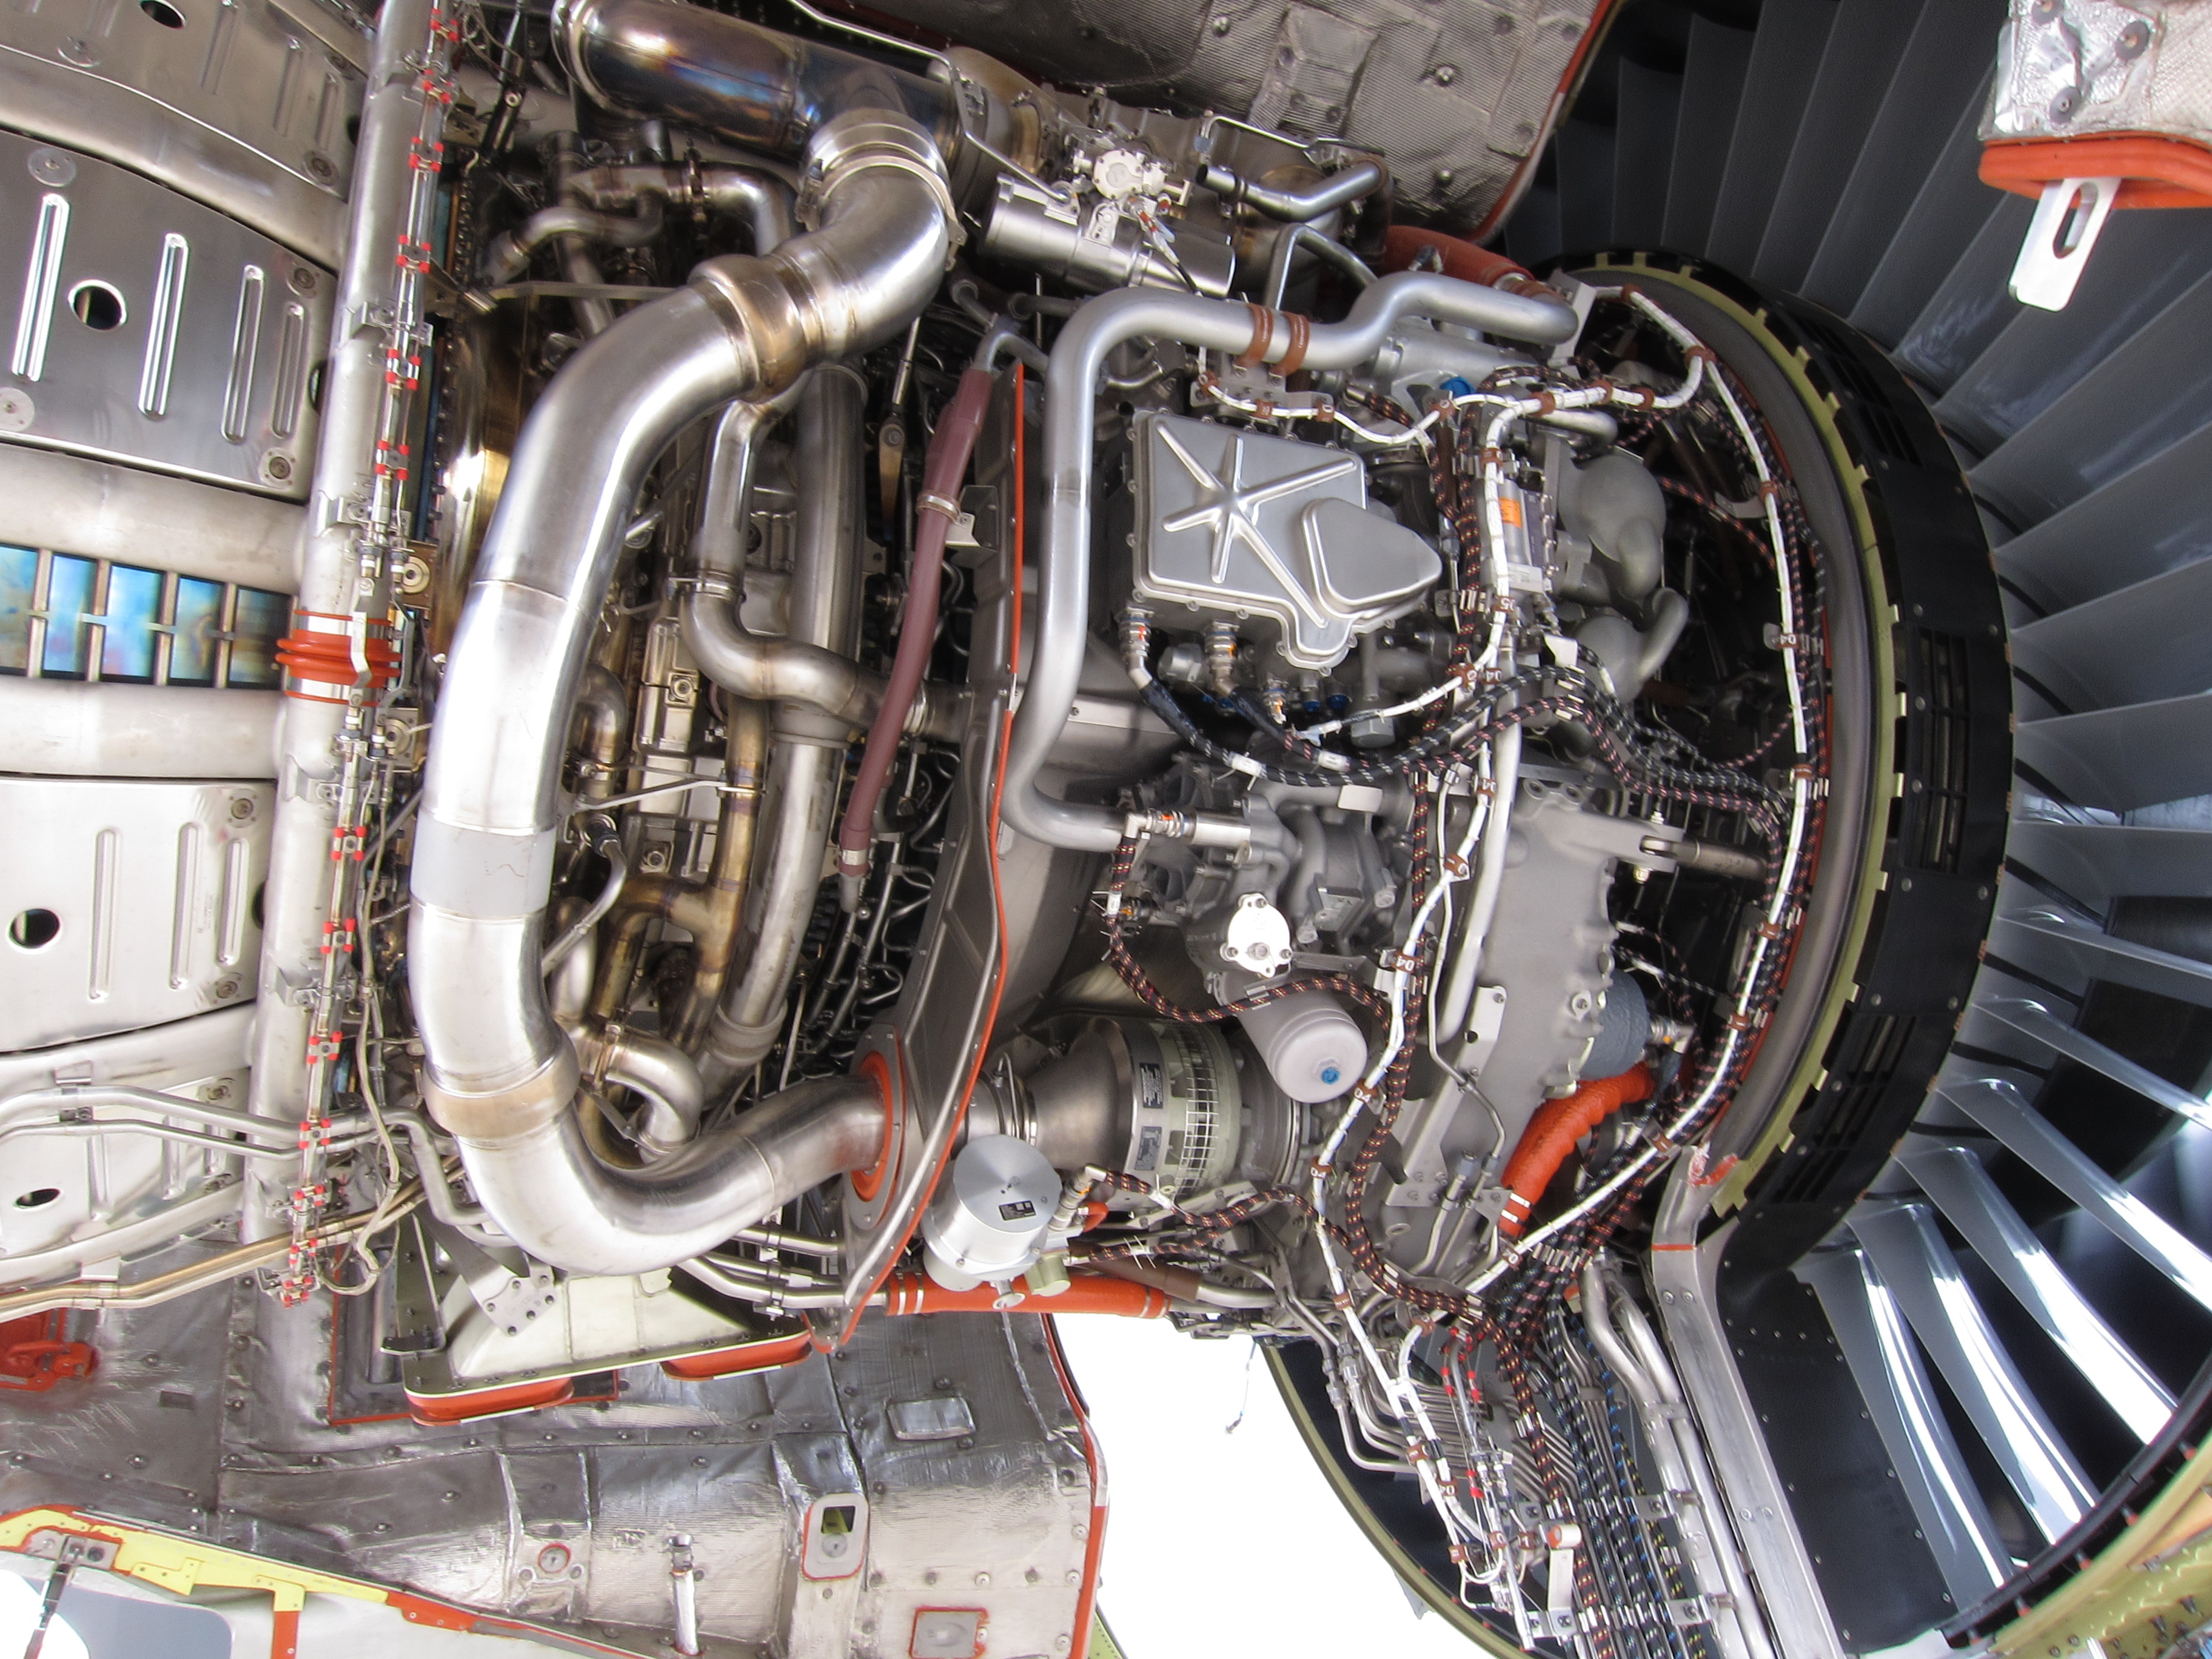
\includegraphics[height=496bp]{portada.jpg}};
 \end{scope}
}{%
 \fill[studiumLight!40!white] (0,89.5) rectangle (595.276,585.5);
 \node[text=studiumInk!45,font=\sffamily\fontsize{10}{13}\selectfont,align=center]
 at (297.638,535){Fotografía definitiva pendiente};
}
\fill[white,opacity=.91] (0,0) rectangle (595.276,89.5);
\fill[studiumInk,opacity=.96] (0,585.5) rectangle (595.276,841.89);
\node[anchor=west,text=studiumInk,font=\sffamily\bfseries\fontsize{18}{20}\selectfont,inner sep=0pt] at (51.223,38.5){STUDIUM};
\node[anchor=east,text=studiumInk,font=\sffamily\fontsize{8}{10}\selectfont,inner sep=0pt] at (544.05,38.5){EN REVISIÓN};
\fill[studiumCyan] (51.223,61.5) rectangle (80.8,63.7);
\node[anchor=west,text=studiumInk,font=\sffamily\fontsize{9}{11}\selectfont,inner sep=0pt] at (89.49,65.5){BIBLIOTECA DE INGENIERÍA};
\node[anchor=west,text=studiumCyan,font=\sffamily\bfseries\fontsize{10}{12}\selectfont,inner sep=0pt] at (51.223,608){#1};
\node[anchor=north west,text=white,text width=493pt,font=\rmfamily\bfseries\fontsize{27}{30}\selectfont,inner sep=0pt] at (51.223,627){#2};
\node[anchor=north west,text=white!82!studiumInk,text width=493pt,font=\sffamily\fontsize{11}{14}\selectfont,inner sep=0pt] at (51.223,730){#3};
\node[anchor=west,text=white,font=\sffamily\bfseries\fontsize{10}{12}\selectfont,inner sep=0pt] at (51.223,774){GRADO EN INGENIERÍA AEROESPACIAL};
\node[anchor=west,text=white!82!studiumInk,font=\sffamily\fontsize{10}{12}\selectfont,inner sep=0pt] at (51.223,789){Universidad de León};
\draw[white!75!studiumInk,line width=.4pt] (51.223,801) -- (544.05,801);
\node[anchor=west,text=white!82!studiumInk,font=\sffamily\fontsize{10}{12}\selectfont,inner sep=0pt] at (51.223,822){2026};
\node[anchor=east,text=white,font=\sffamily\bfseries\fontsize{10}{12}\selectfont,inner sep=0pt] at (544.05,822){Primera edición};
\end{scope}\end{tikzpicture}\null
\end{titlepage}\hypersetup{pageanchor=true}}

\newcommand{\creditosportada}{%
\par\noindent\begin{minipage}{\linewidth}\footnotesize
\textbf{Fotografía de portada.} Detalle del núcleo de un motor General Electric GEnx, Olivier Cleynen (21 de junio de 2011). Fuente: \href{https://commons.wikimedia.org/wiki/File:Detail_of_GEnx_turbofan_engine_core.jpg}{Wikimedia Commons}. Licencia: \href{https://creativecommons.org/licenses/by-sa/3.0/}{CC BY-SA 3.0}.
\par\noindent Se presenta con un recorte de encuadre y superposición de la composición editorial. La fotografía y su adaptación de encuadre mantienen la licencia CC BY-SA 3.0; no se atribuye al fotógrafo respaldo de esta edición.
\end{minipage}\par}

\newcommand{\caso}[2]{\begin{studiumworked}{#1}#2\end{studiumworked}}
\newcommand{\ilustra}[2]{\begin{figure}[htbp]\centering\includegraphics[width=.94\linewidth]{#1.pdf}\caption{#2}\label{fig:#1}\end{figure}}
\newcommand{\fuentes}[1]{\par\medskip\noindent{\footnotesize\textbf{Fuentes y localizadores.} #1}\par}
\newcommand{\apartado}[2]{\par\medskip\noindent\textbf{#1.} #2\par}
\newcommand{\repaso}[2]{\par\medskip\noindent\textbf{Para comprobar la comprensión.} #1\par\noindent\textit{Respuesta razonada.} #2\par}

\hypersetup{pdftitle={Materiales y mantenimiento de motores aeroespaciales},pdfauthor={Studium · Edición de estudio}}
\begin{document}\frontmatter
\portada{MANUAL UNIVERSITARIO}{MATERIALES Y\\MANTENIMIENTO DE\\MOTORES AEROESPACIALES}{Materiales, comportamiento en servicio,\\certificación y aeronavegabilidad}
\chapter*{Presentación y modo de estudio}\addcontentsline{toc}{chapter}{Presentación y modo de estudio}
Este manual desarrolla materiales y mantenimiento de motores aeroespaciales para estudio universitario. La primera parte conecta microestructura, propiedades y daño; la segunda conecta diseño, datos, normativa, ejecución y evidencia. El taller final enseña a construir modelos académicos de programa y control de aeronavegabilidad. Los cuadernos complementarios incluyen 35 problemas originales resueltos, 16 casos académicos, diez simulacros con soluciones y un banco adicional de 36 preguntas tipo test y ocho problemas originales de repaso para examen.

Los ejemplos numéricos emplean valores ficticios salvo identificación expresa de una fuente. No son propiedades certificadas ni límites de un motor. Las figuras son modelos originales y esquemas conceptuales. La fotografía de portada muestra un motor real, pero no transforma los esquemas ni ejercicios en documentación de ese producto.

Cada capítulo presenta objetivos, fundamentos, aplicaciones, una situación trabajada y una pregunta de comprensión. Conviene estudiar primero el modelo y sus hipótesis, resolver después el problema correspondiente y comprobar signos, unidades y límites antes de comparar el resultado. En mantenimiento se añade otra cadena: ámbito, fuente, versión, disposición, configuración y evidencia. Calcular bien un margen no demuestra que la tarea se haya realizado.

\section*{Edición y fecha de referencia}
Primera edición de estudio, 2026. Fecha de corte de las consultas: 18 de octubre de 2026. Se han contrastado las consolidaciones de 1321/2014 de 7 de agosto de 2026, 748/2012 de 22 de febrero de 2026 y 2018/1139 de 2 de agosto de 2026, junto con disposiciones y fuentes señaladas en la bibliografía. Las fechas pertenecen a los textos consultados, no a una promesa de actualización permanente.

\caja{Estado de revisión}{Este manual no ha pasado por una revisión experta independiente. Los cálculos tienen comprobaciones documentadas; la adecuación de modelos, la revisión experta independiente y algunas verificaciones de estado de AD siguen teniendo límites expresos. En particular, la publicación original de FAA AD 2024-14-03 no demuestra por sí sola su estado vigente en octubre de 2026. El registro de verificaciones distingue esos niveles.}
El contenido es formativo. Una solución académica no constituye dato aprobado, autorización de mantenimiento, certificación de trabajo, programa aprobado ni evaluación del estado de una aeronave real. Las decisiones reales requieren los documentos, procedimientos y responsabilidades aplicables al producto y organización.

\section*{Ruta de estudio y diferenciación de fuentes}
Las diapositivas facilitadas por la asignatura y los ejercicios de otros estudiantes ayudan a identificar el estilo y los asuntos preguntados, pero la respuesta de un estudiante \emph{no} equivale a evidencia científica. La teoría se comprobará con definiciones, modelos y fuentes abiertas; en normativa prevalece la versión aplicable del texto oficial. Cada respuesta de examen debería poder explicar: qué se afirma, bajo qué hipótesis, qué evidencia lo sostiene y en qué situaciones deja de ser cierto.

Para practicar se combinan el manual (conceptos), el cuaderno de problemas (método), los simulacros (tiempo y argumentación) y el nuevo banco teórico del mismo cuaderno. El objetivo es maximizar preparación, no prometer que los libros contienen literalmente toda pregunta futura.


\section*{Relación con el material de la asignatura}
Se han utilizado los archivos docentes y hojas históricas aportados para analizar cobertura y dificultades. Las preguntas y ejercicios nuevos no reproducen los de Wuolah. Las copias antiguas de normativa se comparan con fuentes oficiales; se corrigen confusiones detectadas, como identificar 8090 con níquel o intercambiar los modos de fallo adhesivo y cohesivo. La guía docente oficial 2026--2027 se recuperó íntegramente en PDF y se contrastó con las presentaciones \cite{GUIA2026}. \textbf{Hay una discrepancia de evaluación que el estudiante debe conocer:} la guía publica una distribución global de 75\% para pruebas mixtas y 25\% para exposición o defensa de trabajos; la presentación de la asignatura 2026--2027, pp. 8--9, describe \emph{para la parte de Mantenimiento} 40\% de examen a desarrollar/test y 60\% de trabajos, con consideración de trabajos condicionada a una nota de examen de al menos 3.5 sobre 10. La misma presentación indica ponderación de Materiales y Mantenimiento al 50\% cada una y nota mínima de 5 en ambas partes para promediar. \textbf{No se da por resuelta esa diferencia}: una guía general y una presentación de parte no tienen por qué utilizar idéntica base de porcentajes; deben confirmarse la convocatoria, las condiciones y los criterios vigentes con el profesorado. Tampoco los simulacros originales se presentan como modelos oficiales del examen.

No es una publicación oficial de la Universidad de León ni de las autoridades citadas. Las denominaciones académicas identifican el contexto de estudio. Las fuentes consultadas y las obras recomendadas se separan para no atribuir lectura de libros a los que solo se accedió por su ficha bibliográfica.

\chapter*{Símbolos y convenciones}\addcontentsline{toc}{chapter}{Símbolos y convenciones}
\begin{longtable}{p{.18\linewidth}p{.51\linewidth}p{.23\linewidth}}\toprule Símbolo & Significado & Unidad habitual\\\midrule\endhead
$\sigma,\tau$ & Tensión normal y cortante & Pa, MPa\\
$E,G,\nu$ & Módulos elásticos y coeficiente de Poisson & Pa, Pa, adimensional\\
$\varepsilon,\gamma$ & Deformaciones normal y cortante ingenieril & adimensional\\
$a,2a$ & Semilongitud y longitud total de grieta central & m\\
$K_I,K_{IC}$ & Intensidad aplicada y tenacidad válida de modo I en deformación plana & $\mathrm{Pa\sqrt m}$\\
$Y$ & Factor geométrico según convención & adimensional\\
$\sigma_a,\sigma_m,R$ & Amplitud, media y razón mínimo/máximo & Pa, Pa, adimensional\\
$N,n_i,D$ & Ciclos, ciclos aplicados y daño lineal & ciclos, ciclos, adimensional\\
$C,m$ & Parámetros de Paris & Según calibración; adimensional para $m$\\
$Q,R_g,T$ & Energía de activación, constante molar y temperatura & J/mol, J/(mol K), K\\
$\dot\varepsilon$ & Tasa de deformación & $\mathrm{s^{-1}}$\\
$V_f,\rho$ & Fracción volumétrica de fibra y densidad & adimensional, $\mathrm{kg/m^3}$\\
$H,C_{uso}$ & Acumulados de horas y ciclos de uso & h, ciclos\\
$\lambda,R(t),A$ & Tasa de fallo/eventos, supervivencia y disponibilidad & tiempo$^{-1}$, adimensional, adimensional\\\bottomrule
\end{longtable}
Un símbolo puede tener usos distintos entre disciplinas. La razón de carga $R$ no es la constante molar $R_g$ ni la función de fiabilidad $R(t)$. Cada ecuación define su contexto. Las longitudes de grieta se expresan en metros al combinar MPa y $\mathrm{MPa\sqrt m}$. En los resultados decimales de los cuadernos pueden coexistir punto de salida de cálculo y coma tipográfica; no son separadores de miles.

\bigskip\creditosportada

\tableofcontents\listoffigures\listoftables
\mainmatter
\part{Materiales y comportamiento en servicio}
\chapter{Materiales, microestructura y servicio}
\label{ch:01}
\objetivos{Explicar la cadena proceso--estructura--propiedad--prestación; reconocer las familias de materiales y formular una selección ligada a un componente y a su misión.}
\section{La pregunta de ingeniería}
Elegir un material para un aeromotor significa decidir qué combinación de masa, rigidez, resistencia, tolerancia al daño, estabilidad térmica y capacidad de fabricación permite cumplir una función durante un tiempo determinado. La comparación no se resuelve con una clasificación universal de materiales «mejores». Un álabe de fan, un disco de turbina y una junta de estanqueidad comparten motor, pero tienen geometrías, solicitaciones y modos de fallo distintos.

La \textbf{propiedad} es una respuesta medida bajo condiciones definidas. La \textbf{prestación} corresponde al componente: una misma aleación puede dar prestaciones diferentes según su forma, tratamiento, acabado, unión y temperatura. La \textbf{microestructura} incluye fases, tamaños y orientación de granos, precipitados, dislocaciones y defectos. El \textbf{proceso} de fabricación determina gran parte de esa estructura. El mantenimiento observa cómo evoluciona el conjunto durante el servicio.

El razonamiento debe recorrer ambas direcciones. Desde el proceso se predicen tendencias de estructura y propiedades; desde una anomalía en servicio se investiga qué mecanismo y qué historia podrían explicarla. Encontrar una grieta no demuestra por sí solo que el material sea inadecuado: puede haber sobrecarga, vibración, corrosión, daño de fabricación o interacción de varias causas.
\section{Familias de materiales y enlaces}
Los metales y aleaciones presentan enlace metálico y permiten, en muchos casos, deformación plástica mediante movimiento de dislocaciones. Las cerámicas suelen combinar enlaces iónicos y covalentes, elevada estabilidad térmica y limitada plasticidad a temperatura ambiente. Los polímeros contienen cadenas y su respuesta depende de la movilidad molecular, la temperatura y el tiempo de carga. En los compuestos se combinan fases con funciones complementarias y una interfaz que transmite esfuerzos.

Estas son tendencias, no reglas suficientes para seleccionar. Hay metales de baja densidad, cerámicas compuestas tolerantes a ciertos daños y polímeros reforzados muy rígidos en una dirección. La porosidad, la humedad o una orientación desfavorable pueden modificar por completo una comparación basada solo en la composición química.
\caja{Una condición siempre acompaña al dato}{No basta con escribir «resistencia: 900 MPa». Deben identificarse el ensayo, la dirección, el estado metalúrgico, la temperatura, la velocidad de deformación y la base estadística. Un valor típico de una ficha no es automáticamente un valor admisible de diseño.}
\section{Cristales, defectos y endurecimiento}
En un cristal, los átomos ocupan posiciones ordenadas. Las vacantes son defectos puntuales; las dislocaciones, defectos lineales; los límites de grano y las interfaces, defectos superficiales. La palabra defecto describe una desviación estructural, no necesariamente un defecto rechazable en una inspección. La plasticidad de muchos metales sería muy difícil de explicar sin dislocaciones.

El endurecimiento por solución sólida dificulta su movimiento mediante átomos de soluto. La deformación en frío aumenta la densidad de dislocaciones. La precipitación introduce obstáculos cuyo tamaño, distribución y coherencia importan. Los límites de grano también obstaculizan el deslizamiento, de modo que reducir el tamaño de grano puede aumentar el límite elástico dentro del dominio habitual de la relación de Hall--Petch:
\begin{equation}\sigma_y=\sigma_0+k_y d^{-1/2}.\label{eq:hallpetch}\end{equation}
Aquí $d$ es un tamaño medio de grano y $k_y$ tiene unidades de tensión por raíz de longitud. No se extrapola esta relación a cualquier escala ni a cualquier temperatura. A alta temperatura, los límites pueden favorecer difusión y deslizamiento, por lo que una microestructura favorable frente a fluencia puede diferir de otra favorable frente a cedencia a temperatura ambiente.
\section{Propiedades específicas y restricciones}
Para comparar masa se emplean cocientes como $E/\rho$ y $\sigma/\rho$, llamados módulo y resistencia específicos. Su utilidad depende del problema. Una barra limitada por tracción y una viga limitada por flecha no conducen al mismo índice de material, porque la geometría entra con potencias diferentes.

Para una barra de longitud $L$, carga $F$ y tensión admisible $\sigma_{\rm adm}$, $A\geq F/\sigma_{\rm adm}$. Su masa mínima idealizada es
\begin{equation}m=\rho A L\geq FL\frac{\rho}{\sigma_{\rm adm}}.\label{eq:seleccionbarra}\end{equation}
El resultado justifica maximizar $\sigma_{\rm adm}/\rho$ solo cuando las hipótesis de barra, carga, longitud y criterio resistente se mantienen. Si existe una restricción de rigidez, de temperatura o de tamaño mínimo fabricable, la conclusión puede cambiar.
\caso{M01. Una comparación que depende del criterio}{Dos materiales ficticios tienen $(\rho_A,\sigma_{\rm adm,A})=(2800\,\mathrm{kg/m^3},280\,\mathrm{MPa})$ y $(\rho_B,\sigma_{\rm adm,B})=(4500\,\mathrm{kg/m^3},600\,\mathrm{MPa})$. Para la barra idealizada, los cocientes $\rho/\sigma_{\rm adm}$ son $1.0\times10^{-5}$ y $7.5\times10^{-6}\,\mathrm{s^2/m^2}$. La solución B pesa un 25\,\% menos bajo ese único criterio, aunque su densidad es mayor. No se ha comprobado rigidez, corrosión, coste ni temperatura. El ejemplo demuestra por qué la densidad aislada no decide la masa de la pieza.
\par\textbf{Desarrollo para comparar tu intento.} Para una barra gobernada solo por tracción, $A=F/\sigma_{adm}$ y $m=\rho AL=(\rho/\sigma_{adm})FL$. Al comparar igual carga y longitud, se cancelan $F$ y $L$; gobierna el cociente densidad/resistencia admisible, no densidad aislada.

\begin{enumerate}

\item Convertir el primer límite de MPa a Pa antes de dividir.

\[\fitmath{\mathrm{ratioA}=\frac{2800}{280000000}\approx 1\times10^{-5}\,\mathrm{s^{2}/m^{2}}}\]

\item Repetir con el segundo material.

\[\fitmath{\mathrm{ratioB}=\frac{4500}{600000000}\approx 7{,}5\times10^{-6}\,\mathrm{s^{2}/m^{2}}}\]

\item Dividir los factores para comparar masas a igual requisito.

\[\fitmath{\mathrm{massRatio}=\frac{\frac{4500}{600000000}}{\frac{2800}{280000000}}\approx 0{,}75\,}\]

\item La reducción fraccional se expresa en porcentaje multiplicando por cien.

\[\fitmath{\mathrm{saving}=1-\frac{\frac{4500}{600000000}}{\frac{2800}{280000000}}\approx 0{,}25\,}\]

\end{enumerate}

}
\section{Cómo conectar el capítulo con el mantenimiento}
La selección necesita prever qué daño es plausible y cómo se detectará. Una pieza resistente pero difícil de inspeccionar puede exigir otra estrategia de vida. Un recubrimiento protege el sustrato, pero introduce interfaces y mecanismos de desprendimiento. Una reparación puede alterar tensiones residuales y condiciones superficiales; por eso no se evalúa exclusivamente con la composición nominal de la pieza.

La secuencia de trabajo consiste en definir función y condiciones, enumerar modos de fallo, elegir modelos y datos, comparar alternativas, considerar fabricación e inspección y documentar incertidumbres. Se revisa cuando cambia la misión o aparece evidencia nueva. El análisis de servicio se desarrolla en los capítulos~\ref{ch:03}--\ref{ch:06}; la traducción a tareas y registros, en los capítulos~\ref{ch:17} y~\ref{ch:25}.
\ilustra{cadena-material}{Cadena de decisión desde fabricación hasta seguimiento en servicio. Esquema conceptual original.}
\section{Método de selección para preguntas de examen}
No se selecciona un material únicamente por densidad, temperatura máxima o límite elástico: hay que identificar la condición de diseño que gobierna. Si una barra de longitud fija se dimensiona por tensión admisible, la masa idealizada es proporcional a $\rho/\sigma_{\rm adm}$; si el requisito dominante es rigidez o vida a fatiga, debe cambiarse el criterio. Trabajar por debajo de $200\,^{\circ}\mathrm C$ no descarta todos los metales ni garantiza que cualquier polímero funcione: intervienen temperatura de servicio, tiempo, ambiente, carga y estabilidad del material.

\paragraph{Autocomprobación razonada.} ¿Una aleación más densa produce necesariamente mayor masa final? No, porque puede requerir menor sección. ¿Un módulo alto prueba elevada tenacidad? No, son propiedades distintas. ¿Un valor típico es una tensión admisible? No, faltan las condiciones y la base de diseño. Estas distinciones son esenciales en las preguntas de selección de materiales.


\section{Seleccionar significa traducir una función a restricciones}
Antes de buscar una aleación se escribe la función: transmitir fuerza, contener presión, mantener una holgura, resistir una temperatura o proteger un sustrato. Se identifican restricciones que no pueden negociarse, variables que el diseñador puede cambiar y un objetivo medible. La menor densidad solo es un objetivo indirecto: lo que interesa puede ser la masa de una pieza que satisfaga todas las restricciones.

Para una barra a tracción de longitud fija, carga $F$ y tensión admisible académica $\sigma_{adm}$, el área mínima resistente es $F/\sigma_{adm}$ y la masa mínima es $\rho FL/\sigma_{adm}$. Bajo estas hipótesis interesa una razón $\sigma_{adm}/\rho$ alta. Si gobierna el alargamiento máximo, $\Delta L=FL/(EA)$ conduce a una masa proporcional a $\rho/E$. Una clasificación por resistencia específica puede cambiar al imponer rigidez. Si gobierna pandeo, la forma de sección y la longitud entran de otro modo; no se reutiliza automáticamente el mismo índice.

La tensión admisible del ejercicio no debe confundirse con un valor de catálogo sin factores, estadística ni condiciones. En un motor, además, las propiedades pueden depender de temperatura, tiempo, dirección y estado superficial. Un material más resistente puede exigir un tratamiento más complejo o ser menos tolerante a un defecto. La selección final necesita comprobar el mecanismo que realmente limita la pieza.
\section{Dispersión, escala y trazabilidad del dato}
Una probeta pulida y pequeña no reproduce todas las condiciones de una pieza con taladros, uniones y una superficie expuesta a ambiente. El volumen sometido a tensiones elevadas, el tamaño de defecto, la orientación del producto y la secuencia de fabricación pueden modificar la población relevante. No se obtiene una propiedad de diseño añadiendo simplemente la palabra «aeronáutico» a un valor medio.

Una ficha útil identifica composición o especificación, forma de producto, dirección, tratamiento, temperatura, método de ensayo y estadística del dato. También distingue valor nominal, mínimo especificado y admisible de diseño. Si faltan esas condiciones, la comparación puede servir para preselección, pero no para justificar resistencia o vida. El historial de una pieza añade otra capa: un mismo número de aleación no demuestra que dos piezas hayan vivido la misma exposición térmica o corrosiva.
\repaso{Dos materiales tienen igual módulo específico. ¿Pueden intercambiarse en un disco?}{No. Esa igualdad solo compara una combinación de dos propiedades. El disco también exige resistencia, fatiga, tenacidad, comportamiento térmico, procesabilidad, control de defectos y datos de diseño aplicables. La geometría y las condiciones de servicio deben permanecer en el análisis.}

\resumen{\textbf{Autocomprobación.} ¿Una aleación más densa produce siempre una pieza más pesada? No: importa el criterio que determina la sección. ¿Un grano fino mejora siempre la vida a alta temperatura? No: hay que identificar el mecanismo dominante. ¿Una propiedad típica es un admisible? No: faltan condiciones, dispersión y criterios de diseño.}
\fuentes{Material docente de introducción, pp. 1--34; FAA--General, cap. 7 \cite{FAA-G}; módulos de respuesta elástica de Roylance \cite{MIT-ELAS}.}

\chapter{Comportamiento mecánico y estados tensionales}\label{ch:02}
\objetivos{Distinguir magnitudes nominales y verdaderas, manejar el tensor de tensiones y seleccionar una idealización constitutiva compatible con el ensayo.}
\section{Del ensayo a la curva}
En un ensayo uniaxial, la fuerza se transforma en tensión ingenieril mediante el área inicial, $s=F/A_0$, y la elongación en deformación ingenieril mediante $e=(L-L_0)/L_0$. La curva reúne respuesta elástica, posible cedencia, endurecimiento y eventual estricción. El máximo de tensión ingenieril es la resistencia a tracción; no debe confundirse con el inicio de la plasticidad ni con la tensión local de rotura.

Si la deformación es uniforme y se aproxima el volumen como constante durante la plasticidad, $AL=A_0L_0$. De ahí se obtiene la tensión verdadera $\sigma=F/A=s(1+e)$ y la deformación logarítmica $\varepsilon=\ln(1+e)$. Estas conversiones dejan de describir por sí solas el campo local cuando se inicia la estricción. Aplicarlas a la elongación total de una probeta estrangulada puede dar una apariencia de precisión sin un modelo adecuado.
\begin{equation}\sigma=s(1+e),\qquad\varepsilon=\ln(1+e)\quad\text{(deformación uniforme).}\label{eq:verdaderas}\end{equation}
\section{Elasticidad, plasticidad y energía}
La elasticidad describe una deformación recuperable al retirar la carga. La plasticidad añade deformación permanente. En el régimen uniaxial lineal, $\sigma=E\varepsilon_e$; si aparece plasticidad, la deformación total se descompone como $\varepsilon=\varepsilon_e+\varepsilon_p$ bajo pequeñas deformaciones. Un límite convencional al 0,2\,\% se determina con una recta paralela a la pendiente elástica desplazada una deformación de $0{,}002$, no con una pérdida del 0,2\,\% de la carga.

La densidad de energía elástica en carga uniaxial lineal es el área bajo la recta:
\begin{equation}u_e=\int_0^{\varepsilon_e}E\eta\,d\eta=\frac12 E\varepsilon_e^2=\frac{\sigma^2}{2E}.\label{eq:energiaelastica}\end{equation}
Tiene unidades de $\mathrm{J/m^3}$, equivalentes a pascales. La energía por volumen absorbida en un ensayo completo no es la tenacidad a fractura $K_{IC}$, que emplea otra geometría y otras unidades. Tampoco el módulo $E$ cuantifica directamente resistencia: es una pendiente de rigidez constitutiva.
\ilustra{tension-deformacion}{Curva esquemática de tensión ingenieril, descarga elástica y deformación residual. Los valores solo ilustran el modelo.}
\section{Tensión como tensor}
La fuerza por unidad de superficie depende de la orientación del plano. En pequeñas deformaciones y sin pares internos, el estado se representa mediante un tensor simétrico $\boldsymbol\sigma$. La tracción sobre un plano con normal unitaria $\mathbf n$ es $\mathbf t=\boldsymbol\sigma\mathbf n$. La tensión normal es $\sigma_n=\mathbf n^T\boldsymbol\sigma\mathbf n$ y la componente tangencial es la diferencia entre la tracción y esa componente normal.

Las tensiones principales son los autovalores del tensor; sus direcciones son planos sin cortadura. Para un estado plano $(\sigma_x,\sigma_y,\tau_{xy})$,
\begin{equation}\sigma_{1,2}=\frac{\sigma_x+\sigma_y}{2}\pm\sqrt{\left(\frac{\sigma_x-\sigma_y}{2}\right)^2+\tau_{xy}^2}.\label{eq:principales}\end{equation}
La tensión plana supone $\sigma_z=\tau_{xz}=\tau_{yz}=0$; puede aparecer deformación transversal por efecto de Poisson. La deformación plana impone $\varepsilon_z=\gamma_{xz}=\gamma_{yz}=0$ y, en general, origina $\sigma_z\ne0$. Estas idealizaciones no son intercambiables, particularmente junto a una grieta.
\section{Criterios y concentraciones}
Para materiales metálicos dúctiles aproximadamente isótropos se emplean criterios de inicio de cedencia como von Mises. En tensión plana,
\begin{equation}\sigma_{\rm VM}=\sqrt{\sigma_x^2-\sigma_x\sigma_y+\sigma_y^2+3\tau_{xy}^2}.\label{eq:mises}\end{equation}
La comparación $\sigma_{\rm VM}\leq\sigma_y$ no es un criterio universal de rotura y no basta para un compuesto anisótropo, un material frágil o una pieza con grieta. La tensión hidrostática y la triaxialidad adquieren importancia en otros mecanismos.

Una entalla introduce $K_t=\sigma_{\max}/\sigma_{\rm nominal}$ en un análisis elástico concreto. El valor depende de geometría y definición de la tensión nominal. No es el mismo parámetro que $K_I$, cuyo significado y unidades se estudian en el capítulo~\ref{ch:03}. Si el máximo local induce plasticidad, la multiplicación puramente elástica no reproduce la distribución real.
\caso{M02. Estado plano y margen de cedencia}{Para datos ficticios $\sigma_x=120$, $\sigma_y=40$ y $\tau_{xy}=30\,\mathrm{MPa}$, las tensiones principales son $80\pm50$: $130$ y $30\,\mathrm{MPa}$. Von Mises da $\sqrt{13900}=117{,}90\,\mathrm{MPa}$. Si se adopta $\sigma_y=240\,\mathrm{MPa}$, el cociente $\sigma_y/\sigma_{\rm VM}=2{,}036$ es un factor de comparación respecto a ese criterio de cedencia. No es un factor de seguridad frente a fatiga o fractura. La traza $130+30=120+40$ ofrece una comprobación independiente de la transformación.}
\section{Temperatura, tasa y dispersión}
El ensayo debe describir velocidad de deformación y temperatura porque los mecanismos activados térmicamente pueden cambiar la curva. Una ley ajustada en carga lenta puede no representar un impacto. Un ensayo de dureza estima resistencia a penetración bajo condiciones específicas; una conversión a resistencia a tracción es una correlación y necesita validación para la familia y el estado del material.

La dispersión entre probetas exige distinguir valor medio, percentil y límite inferior de una población. Un gráfico de catálogo no contiene por sí solo la probabilidad de fallo de un componente. Cuando se utilicen valores ficticios en problemas, la interpretación debe permanecer dentro del modelo y no atribuir a una aleación real prestaciones no documentadas.

\section{Del tensor a la orientación de un plano}
La tensión sobre un plano de normal unitaria $\mathbf n$ se obtiene mediante $\mathbf t=\boldsymbol\sigma\mathbf n$. Su componente normal es $\sigma_n=\mathbf n\cdot\mathbf t$ y la tangencial es $\mathbf t-\sigma_n\mathbf n$. La tensión no es un vector único asociado al punto: cambia con el plano. Esta distinción explica por qué una sola lectura nominal no describe todos los planos potenciales de daño.

Para una rotación plana de ángulo $\theta$, las componentes se transforman como
\begin{align}
\sigma_{x'}&=\frac{\sigma_x+\sigma_y}{2}+\frac{\sigma_x-\sigma_y}{2}\cos2\theta+\tau_{xy}\sin2\theta,\\
\tau_{x'y'}&=-\frac{\sigma_x-\sigma_y}{2}\sin2\theta+\tau_{xy}\cos2\theta.
\end{align}
La condición de cortante nulo proporciona los planos principales. El círculo de Mohr representa estas relaciones con ángulo doble; confundir $\theta$ con $2\theta$ cambia la orientación física. La suma de principales y otros invariantes permiten verificar que una transformación no ha alterado el estado tensional.
\section{Elasticidad tridimensional y restricción}
En elasticidad isótropa lineal,
\begin{equation}\varepsilon_x=\frac{\sigma_x-\nu(\sigma_y+\sigma_z)}{E},\qquad G=\frac{E}{2(1+\nu)}.\end{equation}
Los tres parámetros $E$, $G$ y $\nu$ no son independientes dentro de ese modelo. Para deformación cortante ingenieril, $\gamma_{xy}=\tau_{xy}/G$; la componente tensorial de deformación es la mitad. Declarar la convención evita un factor dos en energía y transformaciones.

Tensión plana supone que ciertas tensiones fuera del plano son pequeñas; deformación plana supone restringidas ciertas deformaciones. La segunda no equivale a imponer tensión fuera del plano nula. Esta diferencia será esencial al interpretar $K_{IC}$ en el capítulo~\ref{ch:03}. El espesor, las condiciones de contorno y la posición dentro de la pieza determinan qué aproximación es razonable.
\section{Tensión nominal, concentración y plasticidad}
Un factor $K_t$ relaciona un máximo elástico local con una tensión nominal definida. Cambiar la sección de referencia cambia la definición del factor. Si el máximo elástico calculado supera la zona lineal, no basta con truncarlo al límite elástico: aparece redistribución y debe emplearse un modelo compatible. Tampoco un máximo singular en una grieta es una tensión física finita que pueda compararse directamente con resistencia a tracción; la mecánica de fractura ofrece otro descriptor.
\repaso{¿Por qué una deformación transversal distinta de cero no contradice una tensión transversal nula?}{Por el acoplamiento de Poisson. En tracción uniaxial el modelo predice deformaciones laterales aunque las caras estén libres de tensión normal. Las condiciones sobre tensiones y sobre desplazamientos son diferentes.}

\resumen{La curva ingenieril usa geometría inicial; la verdadera requiere información actual y condiciones de conversión. El tensor describe tensiones en planos distintos. Von Mises trata cedencia de materiales compatibles con sus hipótesis; $K_t$ describe concentración geométrica y $K_I$ intensidad del campo de grieta. Son herramientas diferentes.}
\fuentes{Roylance, curvas de ensayo y respuesta elástica \cite{MIT-SS,MIT-ELAS}; FAA--General, cap. 7 \cite{FAA-G}; materiales docentes de introducción y fractura.}

\chapter{Mecánica de fractura y tolerancia al daño}\label{ch:03}
\objetivos{Relacionar energía y campo de punta; diferenciar $K_I$ de $K_{IC}$; calcular un tamaño crítico con una definición explícita de grieta y comprobar las restricciones del modelo.}
\section{Por qué no basta la resistencia nominal}
Una grieta modifica el campo de tensiones y concentra deformación en su punta. La tensión nominal media puede ser inferior al límite elástico y, sin embargo, existir propagación inestable. La mecánica de fractura introduce el tamaño y la geometría del defecto en el análisis. Su objeto no es afirmar que toda indicación sea crítica, sino cuantificar qué combinaciones de carga, defecto y resistencia a propagación son compatibles con el modelo elegido.

En fractura dúctil puede haber nucleación, crecimiento y coalescencia de microcavidades. En fractura frágil la deformación plástica macroscópica puede ser pequeña. Los términos dúctil y frágil describen comportamiento bajo unas condiciones: temperatura, espesor, velocidad de carga y restricciones pueden cambiarlo. La fractografía aporta indicios del mecanismo, pero exige relacionarlos con la historia y no confundir una superficie final de sobrecarga con el origen del daño.
\section{Modos de carga y convención de longitud}
El modo I abre las caras de la grieta; el modo II produce deslizamiento en el plano; el modo III, desgarro fuera de él. Un componente puede presentar modo mixto. Las fórmulas siguientes se limitan al modo I y a mecánica de fractura elástica lineal (MFEL).

Se define $a$ como \textbf{semilongitud} de una grieta central pasante de longitud total $2a$ en una placa idealizada muy ancha. Para una grieta de borde, $a$ suele representar su longitud desde el borde. La fórmula no resuelve esta ambigüedad por el estudiante: cada enunciado debe fijarla.
\ilustra{modos-grieta}{Esquemas de los modos I, II y III y definición de $a$ para una grieta central de longitud total $2a$.}
\section{Criterio energético}
La propagación crea superficie y modifica la energía potencial del sistema. La tasa de liberación de energía es $G=-\partial\Pi/\partial A_c$, con una convención consistente para el área de grieta creada. En un sólido idealmente frágil, el criterio de Griffith iguala energía liberada y energía requerida para crear superficies. En un material real, la resistencia incluye disipación y puede depender de la extensión de grieta; la curva R representa esa evolución.

Para modo I elástico lineal e isotropía,
\begin{equation}G=\frac{K_I^2}{E'},\qquad E'=\begin{cases}E&\text{tensión plana},\\ E/(1-\nu^2)&\text{deformación plana}.\end{cases}\label{eq:gk}\end{equation}
$G$ se mide en $\mathrm{J/m^2}$; $K_I$, en $\mathrm{Pa\sqrt m}$. La equivalencia energética no permite ignorar plasticidad extensa ni anisotropía. La expresión de $E'$ debe corresponder al estado mecánico adoptado.
\section{Intensidad aplicada y resistencia del material}
En un campo singular idealizado de punta, las tensiones elásticas escalan como $K_I/\sqrt{2\pi r}$ multiplicado por funciones angulares. La singularidad no afirma que un material soporte tensión infinita: cerca de la punta existe una zona de proceso que la idealización no resuelve.
\begin{equation}K_I=Y\sigma\sqrt{\pi a}.\label{eq:ki}\end{equation}
El factor $Y$ representa geometría, posición y carga. Puede depender de $a/W$ y no ser constante durante el crecimiento. La tensión $\sigma$ debe estar definida de forma coherente con la solución geométrica, por ejemplo sobre área bruta o neta. Para una placa ideal infinita con grieta central y tracción remota uniforme se adopta $Y=1$.

\textbf{$K_I$ es una solicitación calculada. $K_{IC}$ es una tenacidad crítica de modo I bajo condiciones de deformación plana y validez del ensayo.} El subíndice no es una distinción tipográfica prescindible. Una pieza delgada puede tener otra resistencia aparente $K_c$ dependiente del espesor; no se le atribuye automáticamente el valor $K_{IC}$ de una ficha.
\caja{Criterio de evaluación dentro de MFEL}{La comparación $K_I<K_{IC}$ solo informa sobre inestabilidad de modo I cuando son aplicables el campo elástico, la tenacidad y las condiciones de medida. No demuestra ausencia de crecimiento por fatiga, corrosión bajo tensión o fluencia.}
\section{Tamaño crítico, carga crítica y sensibilidad}
Si $Y$ y la tensión remota se mantienen constantes, imponer $K_I=K_{IC}$ conduce a
\begin{equation}a_c=\frac{1}{\pi}\left(\frac{K_{IC}}{Y\sigma}\right)^2,\qquad\sigma_c=\frac{K_{IC}}{Y\sqrt{\pi a}}.\label{eq:ac}\end{equation}
La derivación muestra que duplicar $\sigma$ divide $a_c$ entre cuatro, mientras que duplicar $K_{IC}$ multiplica $a_c$ por cuatro bajo las mismas hipótesis. Si $Y=Y(a/W)$, se resuelve $Y(a/W)\sigma\sqrt{\pi a}=K_{IC}$ de forma implícita y se comprueba que la raíz está dentro del dominio de la solución geométrica.
\caso{M03. No confundir $a$ con $2a$}{Una placa ideal muy ancha tiene una grieta central pasante de longitud total $4.0\,\mathrm{mm}$, $\sigma=180\,\mathrm{MPa}$, $Y=1$ y una tenacidad supuesta aplicable de $32\,\mathrm{MPa\sqrt m}$. Se usa $a=0.0020\,\mathrm m$. Así, $K_I=180\sqrt{\pi(0.0020)}=14.27\,\mathrm{MPa\sqrt m}$. El tamaño crítico es $a_c=(32/180)^2/\pi=0.01006\,\mathrm m$, es decir, longitud total crítica $2a_c=20.12\,\mathrm{mm}$. La sustitución $180\sqrt{\pi a_c}=32$ cierra el criterio. El resultado no autoriza mantener en servicio el defecto: faltan cargas variables, espesor, entorno y reglas de aceptación.
\par\textbf{Desarrollo para comparar tu intento.} El dato 4 mm es longitud total: la fórmula $K_I=Y\sigma\sqrt{\pi a}$ usa semilongitud. Para el tamaño crítico imponer $K_I=K_{IC}$, dividir por $Y\sigma$, elevar al cuadrado y dividir por $\pi$.

\begin{enumerate}

\item Convertir longitud total y dividir entre dos.

\[\fitmath{a=\frac{0{,}004}{2}\approx 0{,}002\,\mathrm{m}}\]

\item Evaluar intensidad con tensión en MPa y longitud en m.

\[\fitmath{\mathrm{KI}=180\cdot \sqrt{\pi\cdot 0{,}002}\approx 14{,}26798\,\mathrm{MPa\,m^{.5}}}\]

\item Despejar semilongitud crítica.

\[\fitmath{\mathrm{ac}=\frac{{\left(\frac{32}{180}\right)}^{2}}{\pi}\approx 0{,}01006016\,\mathrm{m}}\]

\item Volver a longitud total para comparar con el dato inicial.

\[\fitmath{\mathrm{total}=\frac{2\cdot {\left(\frac{32}{180}\right)}^{2}}{\pi}\approx 0{,}02012033\,\mathrm{m}}\]

\end{enumerate}

}
\section{Zona plástica y validez}
Una estimación de Irwin de la zona plástica de punta es $r_p\simeq(K_I/\sigma_y)^2/(2\pi)$ en tensión plana y, con mayor restricción, $r_p\simeq(K_I/\sigma_y)^2/(6\pi)$ en deformación plana. Son estimaciones, no límites exactos de una zona de geometría universal. La condición de pequeña plastificación exige que esa región sea pequeña respecto al tamaño de grieta, ligamento y dimensiones relevantes.

En ensayos normalizados se emplean condiciones dimensionales de validez. Una expresión de cribado habitual es
\begin{equation}B,\ a,\ W-a\ \gtrsim\ 2.5\left(\frac{K_{IC}}{\sigma_y}\right)^2.\label{eq:espesor}\end{equation}
No debe usarse como una certificación automática de un ensayo: la norma aplicable contiene otras condiciones, geometrías y criterios de carga. Aquí sirve para entender por qué tenacidad alta y límite elástico bajo pueden requerir una probeta grande.

Con $K=32\,\mathrm{MPa\sqrt m}$ y $\sigma_y=400\,\mathrm{MPa}$, la escala derecha vale $16\,\mathrm{mm}$. Una chapa de $3\,\mathrm{mm}$ no satisface ese cribado de espesor. Es incorrecto resolver el problema imponiendo deformación plana y declarar después que se ha comprobado solo porque el enunciado lo pedía.
\section{Cuando la elasticidad lineal resulta insuficiente}
Si la plasticidad no es pequeña pueden necesitarse parámetros elasto-plásticos como $J$ o CTOD. Para una respuesta elástica lineal, $J$ coincide con $G$ bajo las hipótesis correspondientes, pero ello no convierte $J$ y $K$ en símbolos intercambiables en cualquier situación. Una curva de resistencia al desgarro permite estudiar crecimiento estable y la interacción con la rigidez del sistema de carga.

La tolerancia al daño combina tamaño inicial supuesto, crecimiento, detectabilidad y tamaño final admisible. No utiliza el tamaño mínimo nominal de detección como garantía determinista: se consideran probabilidad de detección, accesibilidad, orientación y dispersión. El intervalo de inspección depende del tiempo de crecimiento entre estados justificadamente definidos y de márgenes adicionales.
\ilustra{fractura-critica}{Intensidad aplicada frente a semilongitud de grieta para el ejemplo M03. La intersección ilustra el criterio idealizado, no un límite de mantenimiento real.}

\section{La competencia entre crecimiento de grieta y plasticidad}
La intensidad elástica singular describe un campo intermedio: suficientemente lejos del proceso microscópico de la punta y suficientemente cerca para que domine el término de intensidad. Una estimación de escala de zona plástica en tensión plana es
\begin{equation}r_p\approx\frac{1}{2\pi}\left(\frac{K_I}{\sigma_y}\right)^2.\end{equation}
En una idealización de deformación plana se utiliza un factor diferente, frecuentemente $1/(6\pi)$. Son estimaciones de orden de magnitud. No sustituyen las condiciones completas de un ensayo ni permiten decidir por sí solas que la mecánica lineal es válida. Deben compararse con grieta, ligamento, espesor y gradientes.

Si la plasticidad deja de ser pequeña, energía liberada y deformación plástica se acoplan. Parámetros como la integral $J$ y la apertura de punta pueden ser más adecuados, bajo sus propias condiciones. Una curva de resistencia al crecimiento puede mostrar que la resistencia no permanece constante durante extensión estable. Un valor de $K_{IC}$ no debe usarse como una propiedad universal que cubra cualquier geometría, régimen y mecanismo.
\section{Qué información lleva realmente un factor geométrico}
La expresión $Y\sigma\sqrt{\pi a}$ separa una escala de tensión, una escala de tamaño y una corrección de geometría y carga. $Y$ puede depender de $a/W$, profundidad, relación de aspecto, forma de la superficie y distribución de tensión. Una grieta de borde y una grieta central no comparten automáticamente definición de $a$ ni factor.

Si $Y=Y(a)$, despejar $a_c$ con un valor fijo puede ser inconsistente. Se formula $f(a)=Y(a)\sigma\sqrt{\pi a}-K_c$ y se busca una raíz dentro del dominio físico. La comprobación posterior sustituye la raíz en la ecuación original y verifica ligamento y otras hipótesis. El problema P10 del cuaderno ilustra esta diferencia sin presentar su solución geométrica como válida para toda pieza.
\section{Del defecto observado a una decisión documentada}
La medida de un defecto incluye incertidumbre, orientación, acceso y método. Una indicación superficial puede requerir caracterización adicional; una longitud proyectada no determina siempre profundidad. El análisis usa una idealización explícita de defecto y justifica cómo se relaciona con la evidencia. Después considera las cargas máximas, el crecimiento entre inspecciones y la probabilidad de detección.

La tolerancia al daño integra resistencia residual, evolución del defecto y capacidad de inspección. Si una inspección no cubre una zona crítica, no se compensa solo reduciendo un tamaño inicial en la fórmula. La documentación aplicable determina la actuación real; el cálculo académico enseña a detectar qué hipótesis faltan antes de aceptar una conclusión.
\repaso{Si dos piezas tienen el mismo $K_I$, ¿tienen necesariamente igual seguridad?}{No. Pueden diferir tenacidad aplicable, espesor, ambiente, plasticidad, historia de carga, tensiones residuales y capacidad de detección. La igualdad del parámetro aplicado no iguala todos los mecanismos ni la evidencia.}

\resumen{\textbf{Preguntas de control.} $K_t$ es adimensional; $K_I$ tiene unidades de tensión por raíz de longitud. La longitud total de una grieta central es $2a$. $K_{IC}$ no es un esfuerzo aplicado. La comparación estática no excluye propagación subcrítica. El espesor y el ligamento forman parte de la validez.}
\fuentes{Roylance, \textit{Introduction to Fracture Mechanics}, apartados de Griffith, intensidad y tenacidad \cite{MIT-FRAC}; documentos docentes de fractura, pp. 1--46. El criterio dimensional se explica como cribado; no se afirma haber ejecutado un ensayo ASTM E399.}

\chapter{Fatiga: iniciación, vida y propagación}\label{ch:04}
\objetivos{Definir un ciclo sin ambigüedad; usar curvas S--N y modelos de tensión media con sus límites; integrar la ley de Paris y distinguir vida total de vida de propagación.}
\section{Cómo describir la carga}
La fatiga es daño asociado a cargas variables que puede llevar al fallo con tensiones máximas inferiores a la resistencia estática. Una secuencia puede contener iniciación en superficie o defecto, crecimiento de grietas pequeñas, propagación de una grieta dominante y rotura final. La proporción de vida en cada fase depende del material, superficie, tamaño y espectro. No existe una fracción universal de «vida de iniciación».

Para un ciclo entre $\sigma_{\min}$ y $\sigma_{\max}$ se definen
\begin{equation}\sigma_a=\frac{\sigma_{\max}-\sigma_{\min}}2,\quad\sigma_m=\frac{\sigma_{\max}+\sigma_{\min}}2,\quad R=\frac{\sigma_{\min}}{\sigma_{\max}}.\label{eq:ciclo}\end{equation}
Una carga completamente alternante tiene $R=-1$ y tensión media nula; una carga de cero a un máximo positivo tiene $R=0$ y $\sigma_a=\sigma_m$. La frecuencia, forma de onda, permanencias y ambiente también pueden importar. En motores aparecen ciclos de misión de baja frecuencia y vibraciones de alta frecuencia; su coexistencia exige definir qué fenómeno se modeliza.
\ilustra{ciclo-fatiga}{Definición de máximo, mínimo, amplitud y tensión media en una historia sinusoidal ilustrativa.}
\section{Enfoque tensión--vida}
Una curva S--N relaciona amplitud de tensión y número de ciclos a fallo para condiciones especificadas. Una ley de Basquin puede escribirse $\sigma_a=\sigma'_f(2N_f)^b$, donde el factor dos representa reversiones. También se emplea $\sigma_a=A N_f^b$ con otro coeficiente. No se mezclan coeficientes de ambas convenciones.
\begin{equation}N_f=\left(\frac{\sigma_a}{A}\right)^{1/b},\qquad b<0\quad\text{en el tramo ajustado}.\label{eq:basquin}\end{equation}
No se extrapola una recta de ajuste más allá de la región de datos. Algunas curvas de ciertos aceros muestran una meseta aproximada bajo condiciones concretas; no equivale a vida infinita universal. Corrosión, superficie, tamaño, entallas y temperatura pueden modificarla o eliminar su utilidad como límite. Las aleaciones de aluminio suelen caracterizarse con resistencia a una vida especificada y no con un límite universal.

La dispersión exige declarar si la curva es media o corresponde a una supervivencia determinada. Una regla empírica basada en una fracción de la resistencia a tracción puede orientar un ejercicio expresamente idealizado; no sustituye datos de fatiga de la pieza.
\section{Tensión media, entallas y deformación local}
El diagrama de Goodman modificado aproxima la penalización por tensión media de tracción:
\begin{equation}\frac{\sigma_a}{S_e}+\frac{\sigma_m}{S_u}\leq1.\label{eq:goodman}\end{equation}
$S_e$ representa aquí una resistencia alternante de referencia y $S_u$ una resistencia a tracción compatibles con el modelo. No se generaliza a compresión sin revisar el criterio, ni a plasticidad cíclica intensa. Gerber y Soderberg introducen relaciones diferentes; elegir una no es una equivalencia algebraica, sino una decisión de modelización.

La sensibilidad a entalla se resume a veces mediante $K_f=1+q(K_t-1)$, $0\leq q\leq1$ en el modelo habitual. $K_t$ es geométrico; $K_f$ se vincula al efecto de la entalla en fatiga y depende del material y del problema. No debe aplicarse dos veces un factor si la curva utilizada ya representa el detalle real.

En baja vida con plasticidad local puede emplearse la relación deformación--vida de Coffin--Manson--Basquin:
\begin{equation}\varepsilon_a=\frac{\sigma'_f}{E}(2N_f)^b+\varepsilon'_f(2N_f)^c.\label{eq:coffin}\end{equation}
Los coeficientes requieren ensayos compatibles y el cálculo puede ser implícito. Una tensión nominal elástica no describe necesariamente la amplitud de deformación en una raíz de entalla plastificada.
\section{Daño acumulado y secuencia}
La regla lineal de Miner define $D=\sum_i n_i/N_i$, siendo $N_i$ la vida que asigna el modelo al nivel $i$. El valor $D=1$ se usa como criterio idealizado de fallo. La regla no representa por sí misma efectos de orden, interacción, sobrecargas ni variación del estado superficial. En cargas complejas, el recuento de ciclos exige un procedimiento, por ejemplo rainflow, y una definición de tensión media.
\caso{M04. Un bloque no es una vida}{En un bloque ficticio hay $2000$ ciclos a un nivel con $N_1=100\,000$ y $500$ ciclos a otro con $N_2=20\,000$. Entonces $D_b=2000/100000+500/20000=0{,}045$. La estimación lineal es $1/D_b=22{,}22$ bloques. Tras 22 bloques, $D=0{,}99$; el criterio se alcanzaría durante el bloque siguiente, si se mantiene la misma idealización. El orden de los dos niveles no modifica Miner, aunque sí puede modificar el comportamiento físico.
\par\textbf{Desarrollo para comparar tu intento.} Miner suma fracciones de vida consumidas por cada nivel: $D_b=n_1/N_1+n_2/N_2$. Tras $B$ bloques completos, $D=BD_b$; el criterio ideal unitario da $B=1/D_b$.

\begin{enumerate}

\item Primera fracción de daño del bloque.

\[\fitmath{D1=\frac{2000}{100000}\approx 0.02\,}\]

\item Segunda fracción de daño.

\[\fitmath{D2=\frac{500}{20000}\approx 0.025\,}\]

\item Sumar fracciones, no vidas.

\[\fitmath{\mathrm{Db}=\frac{2000}{100000}+\frac{500}{20000}\approx 0.045\,}\]

\item Despejar bloques para daño unitario.

\[\fitmath{\mathrm{blocks}=\frac{1}{\frac{2000}{100000}+\frac{500}{20000}}\approx 22.22222\,}\]

\item Comprobar el estado tras 22 bloques completos.

\[\fitmath{D22=22\cdot \left(\frac{2000}{100000}+\frac{500}{20000}\right)\approx 0.99\,}\]

\end{enumerate}

}
\section{Propagación: ley de Paris}
En una región intermedia de crecimiento de grietas largas se utiliza
\begin{equation}\frac{da}{dN}=C(\Delta K)^m,\qquad\Delta K=Y\Delta\sigma\sqrt{\pi a}.\label{eq:paris}\end{equation}
$\Delta\sigma=\sigma_{\max}-\sigma_{\min}=2\sigma_a$. El coeficiente $C$ tiene unidades ligadas a la unidad de $a$, de $K$ y al exponente $m$. Un valor calibrado con $\mathrm{MPa\sqrt m}$ no se introduce sin conversión en una ecuación escrita con $\mathrm{Pa\sqrt m}$.

Se distinguen el umbral aparente, la región de Paris y la aceleración cerca de inestabilidad. La razón $R$, el cierre de grieta, las grietas pequeñas, las sobrecargas y el ambiente modifican el crecimiento. La ley de Paris simple no describe automáticamente esas regiones ni una fase de iniciación.

Con $Y$ y $\Delta\sigma$ constantes,
\begin{equation}N=\frac{1}{C(Y\Delta\sigma\sqrt\pi)^m}\int_{a_i}^{a_f}a^{-m/2}\,da.\label{eq:parisint}\end{equation}
Para $m\ne2$ se obtiene
\begin{equation}N=\frac{a_f^{1-m/2}-a_i^{1-m/2}}{(1-m/2)C(Y\Delta\sigma\sqrt\pi)^m};\quad m=2:\ N=\frac{\ln(a_f/a_i)}{C(Y\Delta\sigma\sqrt\pi)^2}.\label{eq:parisclosed}\end{equation}
Con $m>2$, numerador y denominador de la primera expresión son negativos y el resultado es positivo cuando $a_f>a_i$. Esta comprobación de signo evita un error frecuente. Si $Y$ cambia con $a$, se integra numéricamente la expresión completa.
\section{De la propagación al intervalo de inspección}
El tamaño final debe respetar tanto la resistencia frente a inestabilidad al máximo de carga como otros límites aplicables. Un cálculo con $\Delta K$ no sustituye la comprobación de $K_{\max}$. El tamaño inicial de inspección debe tener una base de detectabilidad y no coincidir sin más con «la resolución del equipo».

El intervalo académico puede tomarse como una fracción explícita del crecimiento calculado para explorar márgenes, pero la fracción no se presenta como un requisito reglamentario. Deben declararse fiabilidad de detección, espectro, dispersión del crecimiento y revisión de hipótesis. Los ejercicios de propagación del cuaderno separan claramente el resultado matemático de una decisión de mantenimiento.
\ilustra{sn-paris}{Curvas esquemáticas de tensión--vida y de crecimiento de grieta. Se señalan dominios de ajuste; no son datos de una aleación certificada.}

\section{Ajuste de una curva y coherencia de sus coeficientes}
Si dos puntos compatibles se ajustan con $\sigma_a=A N^b$, el logaritmo da una recta: $\ln\sigma_a=\ln A+b\ln N$. Por tanto
\begin{equation}b=\frac{\ln(\sigma_{a2}/\sigma_{a1})}{\ln(N_2/N_1)},\qquad A=\sigma_{a1}/N_1^b.\end{equation}
Los cocientes de las expresiones para $b$ son adimensionales. El coeficiente $A$ conserva la convención y unidad de tensión del ajuste. Dos puntos permiten determinar dos parámetros, pero no estimar con fiabilidad la dispersión ni demostrar que una ley de potencia sea adecuada fuera del intervalo. Los ensayos que no fallan antes de detenerse no se convierten sin más en fallos a ese número de ciclos: son observaciones censuradas.
\section{Secuencias variables y significado de una permanencia}
Rainflow convierte una historia irregular en un conjunto de ciclos según un algoritmo definido. El resultado debe conservar rangos y tensiones medias pertinentes. No se sustituye una historia por su máximo y mínimo global si contiene numerosos ciclos pequeños y grandes: se perdería la multiplicidad. Después, asignar una vida a cada clase requiere una curva compatible y un tratamiento de tensión media.

Una permanencia a alta temperatura puede introducir relajación, oxidación y daño por fluencia. Dos historias con el mismo número de máximos y mínimos pueden producir diferente daño si una mantiene la carga durante mucho más tiempo. La interacción fluencia--fatiga no queda automáticamente descrita sumando una fracción de Miner y una fracción de tiempo; cualquier regla de interacción necesita su base y límites. En un disco, las variaciones de temperatura y velocidad a lo largo de una misión también cambian el campo local de tensiones.
\section{La integral de Paris como problema de sensibilidad}
Con $m=3$ y $Y$ constante, la vida es proporcional a $1/(C\Delta\sigma^3)$. Un aumento del rango del 10\% reduce la vida del modelo al factor $1/1.1^3\approx0.7513$, manteniendo los tamaños y demás parámetros. Esta sensibilidad explica por qué confundir amplitud con rango puede introducir un error grande. La relación no debe extrapolarse si cambia el dominio de crecimiento o el tamaño final admisible.

El tamaño detectado inicial también pesa mucho: para ese exponente interviene $a_i^{-1/2}$. Reducir arbitrariamente $a_i$ prolonga matemáticamente la vida, pero puede llevar el cálculo al dominio de grietas pequeñas donde el ajuste no representa la física. La inspección y el modelo deben compartir una descripción coherente del defecto.
\ilustra{crecimiento-grieta}{Crecimiento sintético integrado con Paris. La curva acelera al crecer la grieta bajo rango de tensión constante; no incluye la fase de iniciación.}
\repaso{Una solución usa $\sigma_a$ en lugar de $\Delta\sigma$ para Paris con $m=3$. ¿Qué ocurre si todo lo demás permanece fijo?}{Como $\Delta\sigma=2\sigma_a$, la solución usa un impulsor dos veces menor y calcula una vida ocho veces mayor. Corregir la aritmética no basta: también deben comprobarse razón de carga y dominio del ajuste.}

\resumen{Un ciclo necesita máximos y mínimos. S--N estima vida bajo condiciones de ensayo; Paris estima propagación en un dominio distinto. Miner es acumulación lineal aproximada. $K_{\max}$ comprueba inestabilidad y $\Delta K$ impulsa el modelo de crecimiento; ni uno ni otro sustituye al otro.}
\fuentes{Roylance, \textit{Fatigue} y \textit{Introduction to Fracture Mechanics} \cite{MIT-FAT,MIT-FRAC}; materiales docentes de fatiga, pp. 1--37.}

\chapter{Fluencia y vida a alta temperatura}\label{ch:05}
\objetivos{Identificar los mecanismos de deformación dependiente del tiempo; utilizar leyes normalizadas de fluencia y distinguir extrapolación empírica de predicción validada.}
\section{Tiempo, temperatura y tensión}
La fluencia es deformación dependiente del tiempo bajo carga. En materiales metálicos suele adquirir relevancia a temperaturas homólogas elevadas, pero no existe una frontera universal que convierta cualquier comportamiento por encima de una fracción fija de la fusión en fluencia dominante. La temperatura homóloga $T/T_m$ se construye con temperaturas absolutas. En polímeros pueden observarse efectos viscoelásticos significativos a temperaturas mucho más bajas en términos absolutos.

En un ensayo a carga o tensión aproximadamente constante aparecen una deformación inicial y, con frecuencia, tres etapas: primaria, con velocidad decreciente; secundaria o casi estacionaria, con velocidad aproximadamente mínima; terciaria, con aceleración hasta rotura. No todos los ensayos muestran las tres de forma nítida. Bajo carga constante, el cambio de sección puede aumentar la tensión verdadera y contribuir a la aceleración.
\ilustra{fluencia-curva}{Evolución esquemática de deformación de fluencia a temperatura y carga mantenidas. Las regiones delimitan un comportamiento ilustrativo.}
\section{Mecanismos microestructurales}
El deslizamiento de dislocaciones permite deformación plástica; a temperatura suficiente, el ascenso facilita superar obstáculos mediante difusión de vacantes. La competencia entre endurecimiento y recuperación explica parte de la evolución hacia una tasa casi estacionaria. La difusión por el interior del grano y por sus límites puede producir deformación a tensiones relativamente bajas, con distinta dependencia de tamaño de grano.

El deslizamiento de límites necesita mecanismos de acomodación para evitar incompatibilidades. La cavitación puede iniciarse y crecer en límites o interfaces, reducir sección resistente y conducir a rotura. Una microestructura de grano fino, beneficiosa para ciertos comportamientos a temperatura ambiente, puede ofrecer más caminos de difusión o deslizamiento a alta temperatura. Esto ayuda a entender la solidificación direccional y los monocristales en álabes, sin afirmar que sean óptimos para cualquier pieza.

La fluencia coexiste con oxidación, fatiga térmica y cambios de precipitados. En una turbina, el arranque, la permanencia y la parada no son intercambiables con un ensayo a temperatura constante. Las interacciones dependen de secuencia y deben investigarse con datos adecuados.
\section{Ley de potencia y activación térmica}
Para un régimen de mecanismo dominante, una ley de Norton--Arrhenius puede escribirse
\begin{equation}\dot\varepsilon_s=A\sigma^n\exp\!\left(-\frac{Q}{RT}\right).\label{eq:norton}\end{equation}
Las unidades de $A$ dependen de la unidad de tensión. $Q$ y $R$ deben utilizar la misma base molar y unidades energéticas; $T$ es absoluta. El exponente $n$ y la energía aparente $Q$ proceden de ajustes en un dominio, no son constantes universales de todas las temperaturas.

Una forma más segura para comparar estados dentro del mismo régimen usa una referencia:
\begin{equation}\frac{\dot\varepsilon_2}{\dot\varepsilon_1}=\left(\frac{\sigma_2}{\sigma_1}\right)^n\exp\!\left[-\frac{Q}{R}\left(\frac1{T_2}-\frac1{T_1}\right)\right].\label{eq:nortonratio}\end{equation}
Las razones de tensiones son adimensionales y se reduce el riesgo de mezclar MPa y Pa en el coeficiente. Si $T_2>T_1$, el término entre paréntesis es negativo y la exponencial aumenta la tasa cuando $Q>0$: es una comprobación física del signo.
\caso{M05. Sensibilidad a un incremento térmico}{Un modelo ficticio de un único mecanismo tiene $Q=250\,\mathrm{kJ/mol}$ y mantiene la misma tensión al pasar de $900$ a $950\,\mathrm K$. La razón de tasas es $\exp[-250000/8.314462618\,(1/950-1/900)]\simeq5.803$. El resultado muestra una sensibilidad fuerte a la temperatura. No significa que cualquier superaleación aumente exactamente esa proporción: el valor de $Q$ y la permanencia del mecanismo son hipótesis del ejemplo.
\par\textbf{Desarrollo para comparar tu intento.} Al dividir la ley de Arrhenius a igual tensión, se cancela el prefactor y queda $\dot\varepsilon_2/\dot\varepsilon_1=\exp[-Q(1/T_2-1/T_1)/R]$. La diferencia de inversas es negativa al calentar, haciendo positivo el exponente.

\begin{enumerate}

\item Restar inversas de temperaturas absolutas.

\[\fitmath{\mathrm{inverseDifference}=\frac{1}{950}-\frac{1}{900}\approx -5.847953\times10^{-5}\,\mathrm{1/K}}\]

\item Convertir 250 kJ/mol a J/mol.

\[\fitmath{\mathrm{exponent}=\frac{-250000}{8.314462618}\cdot \left(\frac{1}{950}-\frac{1}{900}\right)\approx 1.758368\,}\]

\item Exponenciar para recuperar razón de tasas.

\[\fitmath{\mathrm{rateRatio}=\exp\left(\frac{-250000}{8.314462618}\cdot \left(\frac{1}{950}-\frac{1}{900}\right)\right)\approx 5.802958\,}\]

\end{enumerate}

}
\section{Estimación de deformación y relajación}
Si se aproxima constante la tasa secundaria, $\Delta\varepsilon\simeq\dot\varepsilon_s\Delta t$. Esta operación no calcula automáticamente deformación primaria, terciaria ni tiempo a rotura. Para una tasa $2\times10^{-8}\,\mathrm{s^{-1}}$ durante $100\,\mathrm h$, el incremento es $0.0072$, es decir, $0.72\,\%$; convertir horas a segundos es imprescindible.

En relajación de tensiones, la deformación total impuesta se mantiene aproximadamente constante mientras disminuye la parte elástica y aumenta la parte viscosa. Con elasticidad lineal, $0=\dot\sigma/E+\dot\varepsilon_c$, de donde $\dot\sigma=-E\dot\varepsilon_c$. Un ensayo de relajación no es equivalente a mantener tensión constante. Las juntas y uniones pueden perder precarga aun sin una rotura inmediata de la pieza.
\section{Larson--Miller y extrapolación}
Una correlación de tiempo a rotura emplea
\begin{equation}P=T\left(C_{LM}+\log_{10}t_r\right).\label{eq:larson}\end{equation}
La unidad de $t_r$ se fija en la calibración, habitualmente horas. Dentro del logaritmo se entiende el valor numérico respecto a esa unidad de referencia; no se cambia de horas a segundos conservando el mismo $C_{LM}$. El parámetro no elimina el efecto de la tensión: se construyen relaciones entre $P$ y tensión para material y estado determinados.

Igualar $P$ entre dos temperaturas a una misma tensión permite despejar un tiempo equivalente dentro de la correlación. Si cambian microestructura, mecanismo, oxidación o régimen de tensión, la extrapolación puede perder significado. Un ajuste de datos de ensayos cortos no prueba la vida durante decenas de miles de horas.
\section{Aplicación a aeromotores}
Los álabes calientes necesitan estabilidad microestructural y protección térmica; los discos, además, combinan gradientes, esfuerzos centrífugos y ciclos. El aumento de holguras por deformación puede deteriorar rendimiento antes de que exista rotura. La monitorización de temperatura del gas aporta información operativa, pero no mide directamente la temperatura local del metal ni el daño acumulado.

Para estudiar vida se conserva la historia térmica y mecánica, se definen zonas críticas y se utilizan datos representativos del proceso y del estado metalúrgico. Las inspecciones buscan indicadores compatibles con los mecanismos esperados. No se transforma una correlación académica en una extensión de vida de un componente sin el proceso técnico y documental aplicable.
\section{Monocristales y mecanismos de fluencia: aclaración de examen}
Un monocristal carece de límites de grano internos, pero no queda limitado a fluencia por difusión. También pueden existir mecanismos basados en dislocaciones dentro del grano, como deslizamiento y ascenso activados térmicamente. Es falsa la afirmación de que toda fluencia en un monocristal se produce por difusión, así como la idea de que la ausencia de límites de grano impide la fluencia.

Temperatura y tensión pueden modificar el mecanismo dominante; por ello una ley de Norton o una correlación de Larson--Miller solo se extrapola con justificación de su dominio. \emph{Tiempo para acumular deformación} no significa \emph{tiempo hasta rotura}: las etapas primaria y terciaria, el daño, la oxidación y la historia de cargas pueden alterar la predicción. En un álabe rotatorio, las tensiones centrífugas también requieren justificar distribución de masa, velocidad angular y sección resistente, en lugar de introducir una fuerza global arbitraria.


\section{Mecanismos, tamaño de grano y temperatura homóloga}
La temperatura homóloga $T/T_m$ compara temperaturas absolutas; sirve para orientar qué procesos activados pueden importar, sin fijar una frontera universal de fluencia. El deslizamiento de dislocaciones puede estar limitado por obstáculos; a mayor temperatura, el ascenso asistido por difusión permite superar ciertos obstáculos. Los mecanismos difusivos y el deslizamiento de bordes de grano pueden cobrar importancia con tensiones menores, granos finos y tiempos largos. Los mapas de mecanismos dependen de material y microestructura.

El afinamiento de grano puede mejorar resistencia a cedencia en ciertas condiciones de baja temperatura y, a la vez, aumentar la contribución de mecanismos ligados a bordes a alta temperatura. No hay contradicción: se trata de mecanismos y condiciones diferentes. Esta competencia ayuda a entender el interés de granos orientados o monocristales en ciertos álabes, sin deducir que eliminen todos los procesos de deformación y daño.
\section{Cómo identificar una ley de Norton--Arrhenius}
En un dominio con $\dot\varepsilon=A\sigma^n\exp[-Q/(RT)]$, comparar ensayos a la misma temperatura permite estimar $n$ de la pendiente de $\ln\dot\varepsilon$ frente a $\ln\sigma$. A tensión fija, una gráfica de $\ln\dot\varepsilon$ frente a $1/T$ tiene pendiente $-Q/R$, si $A$ y el mecanismo se mantienen. Un cambio de pendiente puede señalar que una sola ley no describe todo el conjunto.

En una formulación normalizada se escriben cocientes respecto a un estado de referencia; así se reduce el riesgo de confundir unidades del prefactor. Aun así, una buena coincidencia del ajuste no prueba la estabilidad futura de precipitados, oxidación o ausencia de cavitación. El intervalo de calibración debe acompañar a los parámetros.
\Needspace{.48\textheight}
\section{Relajación bajo deformación impuesta}
Bajo deformación total constante y temperatura fija, $\varepsilon_{tot}=\sigma/E+\varepsilon_c$ conduce, si $E$ es constante, a $\dot\sigma=-E\dot\varepsilon_c$. Para Norton a esa temperatura,
\begin{equation}\frac{d\sigma}{dt}=-EA_T\sigma^n,\qquad \sigma(t)^{1-n}=\sigma_0^{1-n}+(n-1)EA_Tt\quad(n\ne1).\end{equation}
Para $n=1$ resulta una disminución exponencial. La tensión se relaja al transferirse deformación elástica a deformación de fluencia. Es distinto de un ensayo a carga constante, donde la tensión no se reduce por esa misma condición de contorno. Con cambios de sección o temperatura hacen falta términos y modelos adicionales.
\repaso{¿Por qué una tasa secundaria baja no demuestra una vida infinita?}{Porque la tasa describe un régimen de deformación, no todo el daño. Pueden evolucionar microestructura, cavidades, oxidación y distribución de tensiones, y puede aparecer fluencia terciaria antes de rotura.}

\resumen{La tasa de fluencia y el tiempo a rotura son magnitudes distintas. La temperatura de las leyes de activación es absoluta. Las constantes de una ley dimensional dependen de las unidades. Una extrapolación solo es defendible dentro de un régimen y con evidencia de su continuidad.}
\fuentes{Roylance, \textit{Dislocation Basis of Yield and Creep} \cite{MIT-CREEP}; materiales docentes de fluencia, pp. 1--27; investigación de superaleaciones de NASA \cite{NASA-SX}.}

\chapter{Corrosión y degradación ambiental}\label{ch:06}
\objetivos{Relacionar ambiente y microestructura con el daño; diferenciar pérdida general de sección, daño localizado y crecimiento asistido por el medio.}
\section{La corrosión como sistema}
La corrosión electroquímica necesita reacciones anódicas y catódicas y un camino de transporte de carga. En una zona anódica se oxida el metal; en la catódica se consumen electrones mediante una reacción compatible con el medio. La distribución puede variar a escala microscópica y no requiere dos piezas distintas. La temperatura, la humedad, el oxígeno, los contaminantes, los depósitos y las diferencias de aireación cambian las velocidades locales.

Una película pasiva puede reducir la velocidad, pero su existencia no garantiza inmunidad. Una discontinuidad, un depósito o un medio que desestabilice la película puede concentrar ataque. En inspección se distingue la cantidad de material perdido de la profundidad y distribución de picaduras: una pérdida media pequeña puede ocultar un defecto local significativo.
\section{Pares galvánicos y geometría}
Al conectar materiales de distinto comportamiento electroquímico en un electrolito, puede acelerarse la disolución del menos noble bajo esas condiciones. La serie galvánica depende del medio y del estado superficial. No se utiliza una tabla genérica como orden universal de compatibilidad.

La relación de áreas importa: un ánodo pequeño conectado a una gran área catódica puede sufrir una densidad de corriente anódica elevada. El aislamiento eléctrico, el control del agua, los sellantes y los recubrimientos forman parte de la prevención. Un recubrimiento defectuoso sobre el ánodo puede, en determinadas configuraciones, concentrar el ataque en una discontinuidad; la protección se estudia como conjunto.
\ilustra{corrosion}{Celda galvánica conceptual: el camino metálico conduce electrones y el electrolito mantiene la continuidad iónica. Las flechas no predicen una velocidad de corrosión ni un único sentido para todas las especies iónicas.}
\section{Corrosión bajo tensión y fatiga-corrosión}
La corrosión bajo tensión requiere una combinación susceptible de material y estado metalúrgico, ambiente y tensión de tracción, que puede incluir tensiones residuales. No es simplemente sumar una pérdida de espesor a un esfuerzo. Pueden aparecer grietas transgranulares o intergranulares según sistema y mecanismo.

Un umbral de intensidad en un medio, a menudo denominado $K_{ISCC}$, depende de condiciones de ensayo y no se intercambia con $K_{IC}$. La fatiga-corrosión combina carga variable y ambiente; puede favorecer iniciación y crecimiento y alterar el significado práctico de una meseta S--N. La frecuencia y las permanencias cambian el tiempo disponible para interacción ambiental.

La fragilización por hidrógeno también depende de susceptibilidad, aporte de hidrógeno y tensiones. Puede relacionarse con procesos de fabricación o mantenimiento, además del ambiente de servicio. Una pieza con aspecto superficial poco alterado puede no estar libre de un mecanismo de fragilización.
\section{Oxidación y corrosión caliente}
A alta temperatura, la formación de óxidos puede proteger o degradar según adherencia, continuidad, estabilidad y transporte a través de la capa. En un régimen controlado por difusión se utiliza a veces una ley parabólica para el espesor de óxido $x$:
\begin{equation}x^2-x_0^2=k_p t.\label{eq:oxidacion}\end{equation}
La constante tiene unidades de longitud al cuadrado por tiempo y depende de temperatura y ambiente. También se usan leyes con ganancia de masa por área; sus constantes no se intercambian con las de espesor. Un régimen lineal, desprendimientos o una transición de mecanismo invalidan el uso indiscriminado de la ley parabólica.

La corrosión caliente puede involucrar depósitos salinos y degradación acelerada de la protección. No se identifica únicamente con «oxidación más rápida». Los recubrimientos de protección y las barreras térmicas tienen capas e interfaces, y pueden fallar por oxidación de la capa de enlace, crecimiento de óxidos, incompatibilidad termomecánica o erosión.
\caso{M06. Una constante necesita su definición}{En un ejercicio isotermo se supone $x_0=0$ y $k_p=4{,}0\times10^{-16}\,\mathrm{m^2/s}$. Tras $100\,\mathrm h$, $x=\sqrt{k_pt}=12{,}0\,\mu\mathrm m$. Tras $400\,\mathrm h$, el espesor es $24{,}0\,\mu\mathrm m$: cuadruplicar el tiempo duplica el espesor en esta ley. No se ha calculado pérdida de metal ni vida del recubrimiento, porque faltan densidades, estequiometría y criterio de fallo.
\par\textbf{Desarrollo para comparar tu intento.} La ley adoptada es $x^2=k_pt$ con espesor inicial cero. Aislar el espesor exige raíz positiva; antes de operar se convierten horas a segundos.

\begin{enumerate}

\item Convertir la primera duración.

\[\fitmath{t_{100}=100\cdot 3600\approx 360000\,\mathrm{s}}\]

\item Aplicar la raíz de producto constante por tiempo.

\[\fitmath{x_{100}=\sqrt{4\times10^{-16}\cdot 100\cdot 3600}\approx 1{,}2\times10^{-5}\,\mathrm{m}}\]

\item Repetir para cuatro veces el tiempo.

\[\fitmath{x_{400}=\sqrt{4\times10^{-16}\cdot 400\cdot 3600}\approx 2{,}4\times10^{-5}\,\mathrm{m}}\]

\end{enumerate}

}
\section{Inspección, prevención y registro}
La prevención combina elección de materiales, diseño de drenajes y uniones, protección superficial, limpieza compatible y control de contaminación. «Limpiar hasta que no se vea» no es un criterio de aceptación. Eliminar corrosión puede reducir sección y debe respetar datos aplicables de reparación y límites de daño.

Se registran ubicación, extensión, profundidad evaluada, método, incertidumbre, fotografías controladas y acciones. La repetición en una zona puede indicar un problema de acceso de humedad o un contacto galvánico no resuelto. En motores se vinculan hallazgos con ambiente de operación, almacenamiento y episodios de contaminación.

\section{La célula electroquímica y la geometría del ataque}
Una célula de corrosión necesita procesos anódico y catódico, conexión electrónica y un medio que permita transporte iónico. En una pareja galvánica importan potenciales en el ambiente real, polarización, área y resistencia del circuito. Un ánodo pequeño conectado a un cátodo grande puede sufrir una densidad de corriente anódica elevada. Invertir las áreas cambia la severidad aunque permanezca la misma pareja nominal.

Los huecos retienen electrolito y favorecen diferencias de aireación; un ataque localizado puede progresar sin una pérdida de masa total llamativa. Por ello la inspección de uniones, zonas de drenaje y superficies ocultas se relaciona con geometría y acceso. Un acabado protege mientras conserva continuidad y compatibilidad; una discontinuidad puede concentrar ataque en una zona pequeña.
\section{Daño ambiental que interactúa con tensiones}
La corrosión bajo tensión requiere una combinación susceptible de material y estado, ambiente y tensión de tracción, incluida la residual. No es simplemente corrosión general acelerada por cualquier carga. La fatiga--corrosión combina ciclos y ambiente y puede modificar iniciación, umbral y crecimiento; las curvas en aire no se trasladan sin más a ese entorno. En ambos casos es esencial identificar mecanismo y condiciones, no solo medir una dimensión final del defecto.

La fragilización por hidrógeno puede relacionarse con procesos de fabricación, protección o servicio, según material y exposición. Un tratamiento o protección que mejore una característica no garantiza ausencia de efectos secundarios. El análisis de fallo examina procedencia, microestructura, superficie de fractura y secuencia temporal; una sola fotografía raramente prueba la causa.
\section{Oxidación protectora y pérdida de protección}
Una película compacta y adherente puede frenar difusión y dar una cinética aproximadamente parabólica. Una película porosa, fisurada o que se desprende puede no mantener esa protección. Los ciclos térmicos introducen incompatibilidades de dilatación y tensiones; el espesor de óxido no equivale directamente a espesor de metal consumido sin conocer composición, densidades y geometría.

En zonas calientes también puede haber corrosión por depósitos y especies ambientales que alteran la película. No se agrupan todos los ataques de alta temperatura bajo un único parámetro de oxidación. En mantenimiento, limpieza e inspección deben ajustarse a datos del producto: una retirada agresiva de depósito puede dañar el sustrato o borrar evidencia.
\repaso{¿Una unión carbono--aluminio es segura frente a corrosión por no contener dos metales?}{No puede concluirse así. El carbono conductor puede participar en un acoplamiento electroquímico con el aluminio en un ambiente adecuado. Se estudian aislamiento, protección, sellado, drenaje y mantenimiento dentro del diseño aplicable.}

\resumen{La corrosión no se caracteriza solo por masa perdida. La geometría y la conexión entre materiales importan. Una ley de oxidación especifica qué magnitud ajusta y bajo qué régimen. $K_{ISCC}$, la resistencia estática y los datos de fatiga en aire no son criterios intercambiables.}
\fuentes{FAA--General, cap. 8, limpieza y control de corrosión \cite{FAA-G}; introducción docente a materiales; protección y materiales de motores en NASA \cite{NASA-CMC}.}

\chapter{Aleaciones metálicas aeroespaciales}\label{ch:07}
\objetivos{Comparar familias de aleaciones sin convertir una denominación comercial en una especificación; relacionar fases, tratamientos y aplicaciones.}
\section{Cómo leer una designación}
La composición nominal identifica una familia, pero la propiedad final exige conocer producto, espesor, proceso, tratamiento y dirección. En aluminio, la serie describe el sistema principal de aleación; el estado de suministro añade información esencial. En titanio se consideran las fases y el tratamiento. En superaleaciones importa también si el producto es forjado, colado, de solidificación direccional, monocristalino o de pulvimetalurgia.

La selección necesita especificaciones y datos admisibles vinculados al producto. Una tabla académica puede organizar tendencias; no constituye una autorización para sustituir una aleación por otra «equivalente» en un motor.
\section{Aceros aeronáuticos e inoxidables}
Los aceros ofrecen combinaciones amplias de resistencia, tenacidad, endurecimiento y coste. En aceros templados y revenidos se ajustan propiedades mediante transformaciones y tratamiento posterior. Los aceros maraging obtienen gran parte del endurecimiento de precipitación en una matriz martensítica de bajo carbono; no son simplemente un acero al carbono con mayor temple.

Los inoxidables se apoyan en la pasividad asociada al cromo, con familias austeníticas, ferríticas, martensíticas y endurecibles por precipitación, entre otras. Su resistencia a corrosión no significa inmunidad frente a picadura o corrosión bajo tensión. La elección de familia depende también de temperatura, magnetismo, soldabilidad y resistencia mecánica.

En ejes, engranajes, elementos de unión y rodamientos importan resistencia a contacto, desgaste, tenacidad y estabilidad dimensional. La alta resistencia puede aumentar sensibilidad a defectos o fragilización, de modo que el tratamiento superficial y el control del proceso no son detalles secundarios.
\section{Aleaciones de aluminio}
Las series 2xxx se asocian principalmente con cobre, las 6xxx con magnesio y silicio, y las 7xxx con zinc como elemento principal, con otros elementos que modifican las fases de endurecimiento. Estas familias incluyen aleaciones tratables térmicamente, pero no todas comparten propiedades ni resistencia a corrosión.

Los estados T3, T6 o T7 describen historias diferentes. El aumento de resistencia por maduración puede implicar compromisos en tenacidad o susceptibilidad ambiental. Un tratamiento sobreenvejecido puede buscar resistencia a corrosión bajo tensión a costa de parte de la resistencia máxima; el compromiso debe justificarse con datos del producto.

Las aleaciones aluminio--litio permiten reducir densidad y modificar rigidez específica, pero plantean cuestiones de anisotropía, tenacidad, fabricación y uniones. La designación 8090 corresponde a una aleación de aluminio--litio; no es una aleación de níquel. Tampoco una temperatura de servicio inferior a $200\,^{\circ}\mathrm C$ descarta «todos los metales»: la selección depende de los requisitos y de la estabilidad de cada aleación.
\section{Titanio: fases alfa y beta}
El titanio presenta fase alfa de estructura hexagonal compacta y beta de estructura cúbica centrada en el cuerpo. Los aleantes estabilizadores y el procesamiento controlan su proporción y morfología. Se distinguen aleaciones alfa, cercanas a alfa, alfa--beta y beta, con respuestas diferentes al tratamiento.

El titanio combina baja densidad relativa frente a aceros y superaleaciones con resistencia específica y buen comportamiento en ambientes adecuados. Sus límites incluyen coste, dificultad de mecanizado, sensibilidad del proceso y compatibilidad a alta temperatura. La interacción con oxígeno durante operaciones calientes puede alterar la superficie; no basta con indicar una resistencia elevada a temperatura ambiente.

En compresores y elementos del fan puede ser atractivo, pero la selección debe considerar temperatura, vibración, impacto, desgaste por contacto y riesgos de ignición o compatibilidad con materiales vecinos. No se deduce una temperatura máxima universal de la palabra «titanio».
\section{Superaleaciones de níquel y cobalto}
En muchas superaleaciones de níquel, una matriz gamma contiene precipitados gamma prima, habitualmente basados en $\mathrm{Ni_3(Al,Ti)}$, que obstaculizan deformación. Otras familias emplean mecanismos y fases diferentes, como gamma doble prima ($\gamma^{\prime\prime}$) en determinadas aleaciones. Carburo, composición de límites y tratamiento influyen en la respuesta. Una fracción de precipitados favorable a una temperatura puede evolucionar durante exposición prolongada.

La resistencia a fluencia, oxidación y fatiga termomecánica hace útiles estas familias en zonas calientes. La densidad y el coste son altos; el diseño de discos y álabes no tiene idénticas prioridades. Las superaleaciones de cobalto pueden ofrecer prestaciones térmicas, ambientales o de desgaste apropiadas en aplicaciones específicas, pero no son un reemplazo universal de las de níquel.

Los álabes monocristalinos eliminan límites de grano de alto ángulo dentro del cristal, aunque mantienen anisotropía y defectos posibles de fabricación. Los discos de grano fino o estructura controlada priorizan otros equilibrios entre fatiga, resistencia y tenacidad. La relación entre microestructura y misión se desarrolla en el capítulo~\ref{ch:10}.
\begin{table}[htbp]\centering\small\caption{Comparación cualitativa de familias. Las prestaciones concretas requieren datos del producto.}\label{tab:familias}
\begin{tabular}{p{.18\linewidth}p{.33\linewidth}p{.37\linewidth}}\toprule
Familia & Ventajas que pueden motivar la selección & Aspectos que deben comprobarse\\\midrule
Aceros & Resistencia, desgaste y diversidad de tratamientos & Masa, corrosión, tenacidad y fragilización\\[4pt]
Aluminio & Densidad baja, fabricación y resistencia específica & Temperatura, fatiga, uniones y ambiente\\[4pt]
Titanio & Resistencia específica y compatibilidad ambiental & Coste, proceso, contacto y límite térmico\\[4pt]
Níquel/cobalto & Servicio caliente y estabilidad microestructural & Densidad, fluencia, recubrimientos y procesado\\\bottomrule
\end{tabular}\end{table}
\section{Una selección explicada}
\caso{M07. Disco y álabe no piden lo mismo}{Se comparan dos piezas ficticias a distinta temperatura: un disco sometido a ciclos centrífugos y un álabe sometido a un gradiente térmico con permanencias. El análisis comienza por fatiga y tolerancia a defectos en el disco, y por fluencia, oxidación y fatiga térmica en el álabe, sin excluir los demás modos. Por ello, escoger la misma familia química no obliga a usar el mismo tamaño de grano ni el mismo proceso. La conclusión es una estrategia de comparación, no una especificación de fabricación.}
\section{Identificación de materiales sin respuestas absolutas}
La aleación 8090 es aluminio--litio, no níquel. Las fases del titanio son alfa, de red hexagonal compacta (HCP), y beta, cúbica centrada en el cuerpo (BCC). Ti--6Al--4V puede presentar microestructuras alfa+beta según proceso y tratamiento: el nombre comercial no permite fijar una microestructura única para cualquier pieza. Los aceros maraging se endurecen principalmente por precipitación, lo cual no garantiza por sí solo resistencia universal a la corrosión o tenacidad suficiente.

Una pregunta sobre material de tren de aterrizaje, fan o estructura de aeronave no admite elegir sin conocer modelo, zona, requisitos y estado metalúrgico. Deben considerarse fatiga, fractura, corrosión, fabricación, temperatura e inspección. La temperatura de fusión de una superaleación no determina por sí sola su máxima temperatura admisible de servicio.


\section{Comparar familias sin convertirlas en recetas}
En aluminio, las series 2xxx y 7xxx suelen relacionarse con endurecimiento por precipitación y elevadas resistencias en estados concretos; las 6xxx ofrecen otras combinaciones de fabricación y propiedades. La familia no determina una resistencia única ni garantiza soldabilidad, resistencia a corrosión o tenacidad. Un estado de tratamiento que maximiza una propiedad puede penalizar otra. Las aleaciones Al--Li añaden posibilidades de menor densidad y modificación del módulo, junto a exigencias de procesado y comportamiento que deben evaluarse en el producto.

En titanio, las proporciones y morfologías de fases alfa y beta dependen de composición e historia térmica. Las propiedades no se deducen únicamente del nombre de la fase: tamaño, distribución y textura importan. Se valoran resistencia específica y compatibilidad térmica, pero también fabricación, comportamiento de superficies y posibles daños por contacto. No se interpreta «resistente a corrosión» como inmunidad en todo ambiente.
\section{Discos y álabes: diferentes compromisos}
Un disco debe soportar esfuerzos asociados a rotación, gradientes térmicos, transitorios y concentraciones, con una población de defectos y una vida controladas. Un álabe caliente añade exposición severa a temperatura, ambiente y vibración y puede usar refrigeración y recubrimientos. Una microestructura adecuada para uno no es automáticamente la mejor para el otro.

Las superaleaciones de níquel combinan matriz y fases de refuerzo estables en un intervalo de servicio; composición, fracción, morfología y estabilidad de precipitados influyen en fluencia y fatiga. El procesado de disco o álabe busca microestructuras diferentes. Las superaleaciones de cobalto también ofrecen combinaciones útiles en aplicaciones calientes, pero no se sustituyen por las de níquel usando solo la temperatura de fusión. El comportamiento de oxidación, corrosión, fabricación y unión completa la comparación.
\section{Aceros, inoxidables y coste de ciclo de vida}
Aceros de alta resistencia pueden resultar apropiados para ejes, engranajes o elementos muy cargados, según diseño. Esa resistencia puede acompañarse de mayor sensibilidad a entallas, ambiente o tratamientos. Los inoxidables reúnen familias microestructurales distintas; la pasividad depende del medio y de la condición superficial. No existe un inoxidable universalmente inmune a picaduras o corrosión bajo tensión.

El coste de adquisición es solo una parte: herramientas, inspección, reparación, disponibilidad de producto, tiempos de suministro y retirada de servicio afectan al coste de ciclo de vida. Una preselección técnicamente prometedora puede descartarse si no existe una ruta de fabricación y control reproducible para la geometría requerida.
\repaso{¿La designación 8090 identifica una superaleación de níquel?}{No: corresponde a una aleación de aluminio--litio. La identificación de familia se verifica antes de discutir propiedades; un número de designación aislado no basta para asignar estado o admisibles.}

\resumen{La designación de aleación es solo parte del dato. Las series de aluminio no sustituyen el estado metalúrgico. Las fases del titanio y los precipitados de las superaleaciones dependen del procesamiento. Temperatura, daño, inspección, fabricación y coste deben compararse conjuntamente.}
\fuentes{FAA--General, cap. 7 \cite{FAA-G}; NASA, desarrollo de superaleaciones de baja densidad \cite{NASA-SX}; materiales docentes de introducción. Para valores de diseño se necesitaría la especificación y su base estadística aplicable.}

\chapter{Tratamientos térmicos y control microestructural}\label{ch:08}
\objetivos{Explicar qué cambia durante un tratamiento y por qué su secuencia importa; distinguir endurecimiento por transformación, precipitación y deformación.}
\section{El tratamiento como historia}
Un tratamiento térmico es una historia de temperatura y tiempo, con condiciones de calentamiento, permanencia, enfriamiento y atmósfera. No se define solo por su temperatura máxima. La sección de la pieza, la transferencia térmica y la carga del horno condicionan gradientes y velocidad de enfriamiento; por eso una receta de probeta no se traslada sin más a un componente masivo.

La microestructura inicial también importa. Dos piezas de la misma composición nominal pueden responder de forma distinta si tienen deformación previa, segregación, tamaño de grano o distribución de fases diferentes. El control incluye trazabilidad del lote, equipo, instrumentación y verificación de propiedades.
\section{Aceros: temple y revenido}
En una secuencia convencional para aceros susceptibles de endurecimiento se austenitiza y se enfría con rapidez suficiente para obtener una estructura martensítica en la zona de interés. La templabilidad describe la capacidad de endurecer en profundidad bajo condiciones de enfriamiento, y no es sinónimo de dureza máxima. Composición, sección y medio de temple intervienen.

El revenido modifica la martensita y los precipitados, alivia parte de las tensiones y ajusta dureza, resistencia y tenacidad. No es una operación decorativa posterior al temple. La combinación final depende de temperatura y tiempo; existen intervalos de fragilización y comportamientos específicos que impiden generalizar que «más revenido siempre mejora todo».

Un enfriamiento desigual puede introducir tensiones residuales, distorsión y grietas. Esas tensiones se suman a las de servicio en el análisis adecuado. Un resultado de dureza satisfactorio en una superficie no demuestra por sí solo uniformidad de propiedades en toda la sección.
\section{Solubilización, temple y precipitación}
En una aleación endurecible por precipitación se busca disolver determinadas fases a una temperatura de solubilización adecuada, enfriar para retener una solución sobresaturada y madurar para desarrollar una distribución de precipitados. El temple de esta secuencia tiene la función de retener soluto; no debe confundirse con la formación de martensita de un acero.

La maduración natural ocurre a temperatura ambiente en sistemas que la presentan; la artificial utiliza una temperatura elevada controlada. La resistencia puede aumentar hasta un máximo y descender con sobreenvejecimiento por evolución del tamaño, coherencia y separación de precipitados. Acelerar el proceso es solo parte de la explicación: el estado alcanzado y sus compromisos también cambian.
\ilustra{tratamiento-termico}{Historia esquemática de solubilización, enfriamiento y maduración, junto a una evolución cualitativa de resistencia. No constituye una receta industrial.}
\section{Tiempo y temperatura no se intercambian libremente}
La difusión y la nucleación compiten con crecimiento y transformaciones. Una temperatura mayor puede acelerar procesos y cambiar las fases presentes. Las correlaciones de tiempo--temperatura se utilizan dentro de dominios calibrados, no como una equivalencia universal entre cualquier tratamiento.

Los diagramas de fases describen estados de equilibrio; los diagramas TTT o CCT incorporan cinética bajo historias concretas. Leer una fracción de equilibrio no demuestra que esa fracción se haya alcanzado en un enfriamiento rápido. El material real puede conservar fases metaestables o gradientes por difusión incompleta.
\section{Procesamiento termomecánico y superficie}
La deformación seguida de recuperación y recristalización modifica densidad de dislocaciones, textura y tamaño de grano. La combinación de forja y tratamiento controla propiedades y defectos de una manera que no se resume solo con la temperatura final. La orientación del flujo de forja puede afectar la respuesta en direcciones distintas.

Los tratamientos superficiales modifican una capa y pueden buscar dureza, resistencia al desgaste, protección ambiental o tensiones residuales favorables. Cementación y nitruración alteran química superficial; granallado introduce deformación y tensiones de compresión; los recubrimientos añaden otra fase e interfaces. Cada proceso requiere comprobar compatibilidad con geometría, defectos y condiciones térmicas posteriores.
\caso{M08. Una reparación puede alterar el estado}{Una zona de una pieza ficticia endurecida por precipitación se calienta localmente durante una intervención. Aunque no cambie su composición nominal, pueden disolverse, crecer o transformarse precipitados. Medir solo dimensiones no demuestra que se conserven las propiedades previas. La evaluación necesita la historia térmica, el material, el estado inicial y los datos de reparación aplicables; el libro no autoriza un tratamiento de recuperación.}
\section{Qué debe documentar un problema}
Un ejercicio de tratamientos debe especificar aleación, estado inicial y objetivo. Si se presenta un diagrama simplificado, debe indicar si es de equilibrio o cinético y qué condiciones representa. Una comparación puede explicar tendencias sin proponer una receta de horno para una pieza aeronáutica.

En fabricación y mantenimiento, la conformidad se apoya en procesos aprobados y registros, no en reproducir de memoria una temperatura de un manual. En el estudio, el objetivo consiste en predecir qué variables cambian, formular hipótesis y reconocer cuándo una medición es insuficiente.
\section{Tratamiento térmico de aleaciones de fundición}
La afirmación de que los aluminios moldeados no admiten tratamientos térmicos es incorrecta. Existen aleaciones de aluminio de fundición, incluidas determinadas Al--Si--Mg, que pueden recibir solubilización, temple y envejecimiento artificial y suministrarse en estados como T6. Su aplicación estructural debe justificarse de forma separada mediante composición, defectos de colada, control de proceso y especificación aplicable.

En una aleación endurecible, el enfriamiento desde solubilización sirve para retener soluto; no equivale al temple martensítico de un acero. La maduración artificial no solo acelera la natural, también modifica el estado de precipitación y el equilibrio entre resistencia, tenacidad y comportamiento ambiental. Una excursión térmica de servicio puede alterar propiedades sin deformación visible; una pieza aparentemente intacta no demuestra conservación de su condición original.


\section{Un diagrama de equilibrio no es una historia de proceso}
Un diagrama de fases representa equilibrios para composición y temperatura bajo las condiciones del modelo. Una línea de enlace permite identificar composiciones de fases coexistentes; la regla de la palanca proporciona sus fracciones en masa cuando el eje de composición usa esa base. Para una aleación global $C_0$ entre $C_\alpha$ y $C_\beta$,
\begin{equation}w_\alpha=\frac{C_\beta-C_0}{C_\beta-C_\alpha},\qquad w_\beta=\frac{C_0-C_\alpha}{C_\beta-C_\alpha}.\end{equation}
Ambas fracciones suman uno y permanecen entre cero y uno dentro de la región bifásica. No son automáticamente fracciones volumétricas: convertirlas exige densidades. Fuera de esa región no se aplica la misma construcción.

Un enfriamiento rápido puede impedir que se alcance el equilibrio. Por eso un diagrama por sí solo no da dureza, tamaño de precipitado o fracción transformada tras un tiempo concreto. La cinética requiere información adicional; las curvas tiempo--temperatura--transformación y las de enfriamiento continuo responden a preguntas diferentes. No se emplean como calendarios intercambiables.
\ilustra{diagrama-fases}{Diagrama binario isomorfo esquemático con región líquido más sólido. Una línea de enlace en la región bifásica permite aplicar la regla de la palanca. No representa un sistema real ni permite definir un tratamiento industrial.}
\section{Precipitación: nucleación, crecimiento y sobreenvejecimiento}
Una secuencia típica de endurecimiento por precipitación parte de una solución sólida sobresaturada que evoluciona durante maduración. Precipitados finos y su relación con la matriz dificultan movimiento de dislocaciones. Al crecer y cambiar coherencia y separación puede variar el mecanismo de interacción y caer la resistencia tras un máximo. La explicación exige identificar la aleación: no todas las secuencias ni fases son iguales.

Una mayor dureza no demuestra automáticamente mejor tenacidad, corrosión bajo tensión o estabilidad térmica. El tiempo de servicio también puede actuar como exposición térmica y modificar el estado obtenido en fábrica. Si una reparación aplica calor local, el efecto puede extenderse más allá de la zona visible; no se restituye una condición solo por observar el mismo color de superficie.
\section{Control del proceso y de sus resultados}
Un proceso reproducible define identificación de pieza, estado inicial, equipos, medio, temperatura, permanencia, transferencia y enfriamiento, además de inspecciones posteriores. Las tolerancias y verificaciones proceden de una especificación aplicable; no se inventan a partir de un esquema docente. La evidencia combina registro del proceso y resultados pertinentes: dimensiones, dureza, microestructura u otros ensayos según la exigencia.
\repaso{Si se aumenta mucho el tiempo de maduración, ¿la resistencia debe seguir creciendo?}{No. Puede alcanzarse un máximo y después sobreenvejecimiento por evolución de precipitados. La respuesta depende de aleación, temperatura y estado previo; la dureza medida debe relacionarse con el requisito específico.}

\resumen{Temple no significa lo mismo en todas las familias. La solubilización y la maduración forman una secuencia. Sobreenvejecer no equivale simplemente a «tratar peor»: puede perseguir otro compromiso, pero requiere datos. Una intervención térmica puede alterar propiedades aunque no deje una deformación visible.}
\fuentes{FAA--General, cap. 7, tratamientos de metales ferrosos y no ferrosos \cite{FAA-G}; materiales docentes de introducción; mecanismos de dislocaciones y recuperación \cite{MIT-CREEP}.}

\chapter{Materiales compuestos, laminados y uniones}\label{ch:09}
\objetivos{Relacionar orientación y transferencia de carga con las propiedades; utilizar reglas de mezcla como modelos limitados e identificar modos de fallo diferenciados.}
\section{Matriz, refuerzo e interfaz}
Un compuesto reúne fases distinguibles para obtener una respuesta que no se describe solo con la suma de sus masas. En un laminado de fibras largas, el refuerzo puede aportar gran rigidez en su dirección, mientras la matriz transmite cortadura, mantiene posición, protege y participa en cargas transversales. Decir que «la matriz nunca soporta carga» es incorrecto. Su contribución cambia con dirección, temperatura, geometría y estado de daño.

Las matrices poliméricas pueden ser termoestables o termoplásticas; su respuesta depende de temperatura, humedad y tiempo. Las matrices metálicas y cerámicas permiten otros intervalos térmicos y mecanismos de transferencia y daño. Un compuesto cerámico con mecanismos de desviación de grieta y extracción de fibras puede tener una respuesta al daño distinta de una cerámica monolítica.
\section{Anisotropía y modelos de mezcla}
Para un compuesto unidireccional ideal con fibras continuas alineadas, unión perfecta y deformación longitudinal igual en ambas fases,
\begin{equation}E_L=V_f E_f+V_m E_m,\qquad V_f+V_m=1.\label{eq:mezclaL}\end{equation}
Se obtiene sumando las fuerzas de fibras y matriz a igual deformación. Para una idealización de igual tensión en serie,
\begin{equation}\frac1{E_T}=\frac{V_f}{E_f}+\frac{V_m}{E_m}.\label{eq:mezclaT}\end{equation}
La segunda expresión es una idealización sencilla y no una predicción exacta de cualquier módulo transversal real. La geometría, las interfaces, vacíos y distribución del refuerzo hacen necesarios modelos o ensayos más representativos. La densidad ideal sin vacíos sí se calcula por promedio volumétrico $\rho=V_f\rho_f+V_m\rho_m$.
\caso{M09. Dirección de las fibras}{Para datos ficticios $V_f=0.60$, $E_f=230$ y $E_m=3\,\mathrm{GPa}$, el modelo longitudinal da $E_L=139.2\,\mathrm{GPa}$. La idealización en serie da $E_T=7.356\,\mathrm{GPa}$. La gran diferencia ilustra anisotropía, no dos resultados rivales para la misma dirección. El resultado transversal debe interpretarse dentro de la idealización, sin atribuirlo a una lámina comercial.
\par\textbf{Desarrollo para comparar tu intento.} La fracción de matriz es $V_m=1-V_f$. En paralelo longitudinal las fases comparten deformación y se suman rigideces ponderadas; en serie transversal comparten tensión y se suman flexibilidades antes de invertir.

\begin{enumerate}

\item Obtener fracción de matriz.

\[\fitmath{\mathrm{Vm}=1-0{,}6\approx 0{,}4\,}\]

\item Sumar las contribuciones longitudinales en las mismas unidades.

\[\fitmath{\mathrm{EL}=0{,}6\cdot 230+0{,}4\cdot 3\approx 139{,}2\,\mathrm{GPa}}\]

\item Sumar flexibilidades transversales y tomar el inverso.

\[\fitmath{\mathrm{ET}=\frac{1}{\frac{0{,}6}{230}+\frac{0{,}4}{3}}\approx 7{,}356077\,\mathrm{GPa}}\]

\end{enumerate}

}
\section{De la lámina al laminado}
Una lámina ortótropa necesita varios parámetros independientes: módulos, coeficientes de Poisson y módulos de cortadura, con relaciones de reciprocidad en elasticidad. Al girar la lámina, cambia la relación entre las componentes de tensión y deformación en los ejes globales. En un apilado, orientación y posición respecto al plano medio determinan respuesta extensional, de flexión y acoplamientos.

La teoría clásica de laminados organiza resultantes como
\begin{equation}\begin{bmatrix}\mathbf N\\\mathbf M\end{bmatrix}=\begin{bmatrix}\mathbf A&\mathbf B\\\mathbf B&\mathbf D\end{bmatrix}\begin{bmatrix}\boldsymbol\varepsilon^0\\\boldsymbol\kappa\end{bmatrix}.\label{eq:abd}\end{equation}
Un laminado simétrico respecto al plano medio tiene $\mathbf B=0$ en esta teoría y sin otros efectos que rompan las hipótesis. «Simétrico» no significa necesariamente «isótropo». Un apilado equilibrado elimina determinados acoplamientos de cortadura, pero tampoco constituye una solución universal frente a todas las cargas.
\ilustra{laminados}{Orientaciones de lámina, secuencia simétrica y estructura sándwich. La representación es conceptual, sin espesores de un producto real.}
\section{Fallo, delaminación y daño por impacto}
Los mecanismos incluyen rotura de fibras, fisuración de matriz, despegue de interfaz, inestabilidad local y delaminación. La resistencia puede depender de tracción o compresión y de dirección. Un criterio de fallo debe declarar qué mecanismos representa. Un único «límite elástico equivalente» de un metal no describe por sí solo una lámina anisótropa.

La delaminación separa capas y puede reducir mucho la capacidad de compresión o flexión sin una abertura superficial evidente. Las tensiones interlaminares se concentran en bordes, uniones y cambios de espesor; un modelo de tensión plana de lámina no las resuelve completamente. El daño apenas visible por impacto exige una estrategia de detección y evaluación compatible.
\section{Sándwich, GLARE y materiales de motor}
Una estructura sándwich separa caras resistentes mediante un núcleo ligero. La separación aumenta la rigidez a flexión con poca masa, pero introduce cortadura del núcleo, aplastamiento, arrugamiento de caras y despegue como modos posibles. No se verifica solo con la tensión longitudinal de las caras.

GLARE es un laminado híbrido de capas metálicas de aluminio y láminas reforzadas con fibra de vidrio. Puede combinar mecanismos de puenteo de grieta y respuesta a fatiga con exigencias de uniones y fabricación. Sus propiedades dependen del grado y apilado; no se le atribuye automáticamente la rigidez de un compuesto de carbono.

En motores pueden emplearse polímeros reforzados en zonas compatibles con su temperatura y ambiente, y compuestos de matriz cerámica en determinadas piezas calientes. Los CMC necesitan considerar oxidación, vapor de agua, recubrimientos ambientales, interfaces y vida; no son «cerámicas que ya no fallan de forma frágil» en cualquier condición.
\section{Uniones adhesivas}
Se distingue \textbf{fallo adhesivo}, situado en la interfaz entre adhesivo y sustrato; \textbf{fallo cohesivo}, dentro del adhesivo; y \textbf{fallo del sustrato}, dentro del material unido. La preparación superficial, contaminación, curado y diseño del extremo influyen en la distribución de esfuerzos.

Para una unión solapada, $F/(bL)$ es una tensión cortante media, no el máximo local. Los extremos pueden presentar concentraciones y esfuerzos de pelado. Aumentar indefinidamente el solape no garantiza un aumento proporcional de resistencia. Las reparaciones adheridas requieren datos, preparación y controles específicos.
\section{Desmontar las trampas habituales de compuestos y adhesivos}
La matriz soporta parte de las cargas y transmite esfuerzos entre fibras: no funciona simplemente como separador pasivo. Termoplásticos y termoestables son familias distintas; un termoestable curado y reticulado no se funde y reprocesa como un termoplástico. La elección debe atender a temperatura de transición vítrea, humedad, módulo y duración de la carga.

GLARE es un laminado híbrido metal--fibra de vidrio, cuya rigidez depende de secuencia de apilado y dirección. No existe un único módulo de GLARE válido para cualquier orientación. En un panel sándwich en flexión, las caras soportan gran parte de la tensión normal de tracción/compresión y el núcleo contribuye especialmente a cortadura y estabilidad de las caras. Los signos de las tensiones cambian con el momento, no se asignan por definición a una cara universal.

En uniones adheridas, fallo \emph{adhesivo} es separación interfacial; fallo \emph{cohesivo}, rotura dentro del adhesivo; y fallo \emph{del sustrato}, rotura del material unido. La resistencia real depende de preparación superficial, espesor, curado, dirección de carga y condiciones ambientales.


\section{De una lámina a un laminado: qué se suma}
Una lámina ortótropa tiene rigideces distintas según dirección y acoplamiento por Poisson. Al girar la lámina se transforma su matriz de rigidez; no se promedian simplemente módulos longitudinal y transversal. En teoría clásica de laminados, bajo sus hipótesis de placa delgada y unión entre capas, resultantes y deformaciones se relacionan mediante
\begin{equation}\begin{bmatrix}\mathbf N\\\mathbf M\end{bmatrix}=\begin{bmatrix}\mathbf A&\mathbf B\\\mathbf B&\mathbf D\end{bmatrix}\begin{bmatrix}\boldsymbol\varepsilon^0\\\boldsymbol\kappa\end{bmatrix}.\end{equation}
$\mathbf A$ reúne rigidez de membrana, $\mathbf D$ la de flexión y $\mathbf B$ el acoplamiento entre ambas. Las unidades son, respectivamente, fuerza por longitud, fuerza por longitud multiplicada por longitud al cuadrado, y fuerza, si se usan las resultantes habituales. La convención de signos de curvatura y del eje de espesor se declara antes de comparar matrices.

Un apilado simétrico respecto al plano medio anula $\mathbf B$ en el modelo ideal porque las contribuciones impares en espesor se cancelan. Eso no elimina todos los acoplamientos posibles dentro de $\mathbf A$ o $\mathbf D$ ni demuestra isotropía. Cambiar el orden de capas puede conservar una rigidez de membrana y modificar flexión. Las propiedades y espesores reales siguen siendo necesarios.
\section{Cargas de matriz, interfaces y daño}
Las fibras pueden dominar una rigidez longitudinal, pero la matriz transmite carga entre fibras, estabiliza y participa en respuesta transversal y cortante. La interfaz determina transferencia y ciertos modos de daño. Bajo compresión, flexión o carga fuera de plano, afirmar que la matriz «no soporta carga» puede ocultar el mecanismo que gobierna.

Fisuración de matriz, rotura de fibra y delaminación pueden aparecer en secuencia e interactuar. Un impacto con huella pequeña puede dejar daño interno relevante; observar la superficie no caracteriza todo el volumen. La resistencia interlaminar y la tenacidad de delaminación describen aspectos distintos y dependen del modo de apertura o cortante. La teoría clásica elástica de placa no resuelve por sí sola el campo tridimensional de un borde libre o un impacto.
\Needspace{.48\textheight}
\section{Sándwich, GLARE y uniones adhesivas}
Separar caras aumenta rigidez a flexión con poca cantidad de material resistente de cara, pero el núcleo debe transmitir cortante y mantener la separación. Arrugamiento, aplastamiento, despegue e infiltración pueden gobernar antes de alcanzar la resistencia nominal de las caras. La ganancia ideal de inercia del problema P25 debe leerse junto a estas limitaciones.

GLARE combina capas metálicas y de compuesto de vidrio en una arquitectura específica; no es cualquier panel con vidrio y aluminio. Las rutas de daño, propagación y reparación dependen de esa arquitectura. En una unión adhesiva, $F/(bL)$ solo es cortante media: extremos del solape y excentricidad introducen concentraciones y pelado. Preparación superficial, curado, espesor, ambiente y compatibilidad de sustratos son parte del sistema resistente.
\repaso{¿Un laminado simétrico y equilibrado es necesariamente isótropo?}{No. Simetría y equilibrio eliminan ciertos acoplamientos bajo condiciones del modelo, pero las rigideces pueden seguir variando con dirección. La isotropía o cuasiisotropía requiere condiciones adicionales sobre el apilado y el comportamiento considerado.}

\resumen{La dirección de carga forma parte de la propiedad. Las reglas de mezcla son modelos con hipótesis, no fichas de laminado. Simetría del apilado y equilibrio no equivalen a isotropía. Adhesivo, cohesivo y sustrato identifican localizaciones distintas del fallo.}
\fuentes{Roylance, \textit{Introduction to Composites} y \textit{Laminated Composite Plates} \cite{MIT-COMP,MIT-LAM}; FAA--General, cap. 7 \cite{FAA-G}; NASA sobre CMC \cite{NASA-CMC}.}

\chapter{Materiales y degradación de aeromotores}\label{ch:10}
\objetivos{Explicar por qué cambian los materiales a lo largo del motor y relacionar cada pieza con sus solicitaciones y mecanismos de daño.}
\section{Un mapa de temperatura y función}
El recorrido del aire y del gas atraviesa fan, compresores, cámara de combustión, turbinas y salida. La temperatura del gas aumenta con la compresión y, especialmente, con la combustión. La temperatura del metal depende además de refrigeración, recubrimientos, transferencia térmica y régimen transitorio. No se iguala automáticamente a una temperatura medida del gas.

La selección se realiza por componente. Una carcasa puede priorizar contención y estabilidad dimensional; un disco, integridad bajo esfuerzos centrífugos y ciclos; un álabe, aerodinámica, vibración y resistencia térmica; un cojinete, contacto, desgaste y lubricación. La exposición al daño por objetos extraños y el acceso de inspección añaden restricciones.
\ilustra{motor-materiales}{Mapa funcional de un turbofán y de familias de materiales que pueden emplearse en distintas zonas. Esquema de tendencias, no despiece de un motor concreto.}
\section{Fan y compresor}
El fan debe combinar masa, rigidez, resistencia centrífuga, vibración e impacto. Según diseño se utilizan aleaciones de titanio, compuestos con protecciones y otras soluciones. El compresor añade incrementos de temperatura, esfuerzos cíclicos y riesgos asociados a rozamientos o ingestión. Las últimas etapas pueden exigir familias de mayor capacidad térmica.

Erosión y depósitos alteran perfiles, holguras y rugosidad; con ello pueden modificar rendimiento y margen de operación. Una pérdida de eficiencia no identifica por sí sola una grieta. Una entalla por impacto puede ser pequeña en masa perdida y relevante para fatiga, por lo que las dimensiones y ubicación del daño importan.
\section{Cámara de combustión y turbina}
La cámara combina llama, gradientes, oxidación, vibración y fatiga térmica. El revestimiento metálico y sus recubrimientos trabajan junto a refrigeración y geometría de orificios. Un deterioro local de refrigeración puede elevar temperatura del metal aunque una medida global siga dentro de una banda habitual.

Los álabes de turbina pueden experimentar fluencia y fatiga termomecánica, además de oxidación, corrosión caliente y erosión. La solidificación direccional orienta granos para reducir ciertos límites transversales; los monocristales eliminan límites de alto ángulo en el cristal, pero exigen control de orientación, porosidad y defectos de colada. No eliminan toda posibilidad de daño ni la necesidad de inspección.
\section{Discos, carcasas y elementos de contacto}
La integridad de un disco necesita gestionar esfuerzos centrífugos, gradientes y ciclos. La resistencia a iniciación y propagación de defectos debe evaluarse junto a la dispersión de fabricación. En un disco de metal procesado por polvo, la limpieza, las inclusiones y la homogeneidad de proceso pueden ser críticas; la composición nominal es insuficiente.

Las carcasas condicionan holguras y alineación. Su dilatación respecto a rotores puede variar durante arranques y paradas, dando lugar a contactos. En cojinetes, la película lubricante, el estado de superficies, la contaminación y la temperatura se relacionan con desgaste, fatiga de contacto y calentamiento. Un análisis de partículas en aceite aporta evidencia de desgaste, pero necesita origen y tendencia.
\section{Barreras térmicas y ambientales}
Una barrera térmica suele combinar sustrato, capa de enlace y capa cerámica con una arquitectura determinada. La diferencia de expansión térmica, el crecimiento de óxidos en la interfaz, el ciclado y los depósitos pueden favorecer desprendimientos. El recubrimiento reduce solicitación térmica bajo condiciones de transferencia determinadas; no garantiza una reducción fija de temperatura en todos los motores.

En ciertos CMC, los recubrimientos ambientales protegen frente a mecanismos químicos, por ejemplo asociados al ambiente de combustión. No debe confundirse protección ambiental con aislamiento térmico, aunque puedan coexistir funciones. La evaluación de una zona sin recubrimiento necesita datos específicos de ubicación y extensión.
\caso{M10. Una subida de temperatura no diagnostica sola}{En un motor ficticio aumenta la temperatura de escape necesaria para mantener un empuje comparable. Entre las hipótesis figuran deterioro de perfiles, mayores holguras, suciedad, cambio de ambiente o error de sensor. Se comparan parámetros corregidos y condiciones de misión antes de atribuirlo a una turbina degradada. Si además aparece un hallazgo de boroscopia, se relaciona su ubicación con la tendencia. El caso enseña a combinar evidencias sin inferir un mecanismo único de una sola señal.}
\section{Del mecanismo al plan de seguimiento}
Un mapa de daño vincula pieza, mecanismo, factor impulsor, indicio y técnica. Para fatiga de un disco puede interesar iniciación en una zona concentradora y un método sensible al defecto esperado; para un revestimiento caliente, la distribución de grietas o pérdida de recubrimiento puede ser la evidencia principal. Los límites reales dependen de los datos de mantenimiento del motor.

La ingeniería de materiales y el mantenimiento se encuentran en la trazabilidad: qué pieza, qué estado, qué historial y qué datos justifican una acción. La modelización académica ayuda a interpretar por qué existe un límite o una inspección; no modifica ese límite ni sustituye la instrucción aplicable.

\section{Un motor impone campos, no una sola temperatura}
La temperatura del gas, la del metal y la de un sensor no son intercambiables. La refrigeración interna y superficial, el espesor, la conductividad y los recubrimientos crean gradientes. Un aumento de temperatura de gas no permite sumar el mismo incremento a todos los componentes. El cálculo térmico también necesita condiciones de contorno, transitorios y radiación cuando sea relevante.

Los gradientes generan deformaciones diferenciales; las restricciones convierten parte de ellas en tensión. En un arranque o parada pueden coexistir tensiones mecánicas y térmicas de signos y distribuciones cambiantes. La compatibilidad entre disco y álabe, holguras con carcasa y evolución del recubrimiento relaciona materiales y diseño térmico. Optimizar una propiedad aislada puede trasladar el problema a otra interfaz.
\section{Microestructura orientada, refrigeración y recubrimiento}
La solidificación direccional reduce ciertas fronteras transversales a la solicitación; un monocristal evita bordes de grano de alto ángulo dentro de la idealización del producto, pero conserva anisotropía cristalina y otros defectos posibles. Orientación, defectos de colada, tratamiento y acabado necesitan control. No equivale a un material sin mecanismos de fallo.

Un sistema de barrera térmica incluye funciones del recubrimiento cerámico, capa de unión y óxido que evoluciona durante exposición, según arquitectura. Diferencias de dilatación, oxidación, erosión y ciclos pueden iniciar pérdida de adherencia. Un recubrimiento desprendido modifica el campo térmico del sustrato; medir solo su espesor medio no describe todas las condiciones de protección. El ejemplo térmico P35 enseña resistencias en serie, sin reproducir una geometría refrigerada real.
\section{Un mapa de daño por componente}
En fan y compresor interesan impacto, erosión, fatiga y degradación aerodinámica; el material y la etapa condicionan la relevancia de cada uno. En cámaras y zonas calientes aparecen ciclos térmicos, oxidación, corrosión caliente, fisuración y degradación de recubrimientos. En discos se estudian fatiga y defectos en un campo centrífugo y térmico. En cojinetes, contacto, lubricación y contaminación exigen otro enfoque.

Este mapa se utiliza para formular preguntas de inspección: dónde, qué mecanismo, qué evidencia y qué método lo puede observar. No convierte una lista de daños posibles en diagnóstico. Dos mecanismos pueden producir señales parecidas; por ejemplo, una pérdida de rendimiento puede deberse a degradación de perfiles, holguras o condiciones de medida. El capítulo~\ref{ch:22} conecta este razonamiento con seguimiento en servicio.
\repaso{¿Por qué una cerámica puede trabajar en una zona caliente y aun así requerir protección ambiental?}{La estabilidad térmica no garantiza resistencia frente a todas las especies del gas, vapor, depósitos, erosión o ciclos. La selección considera química del ambiente y sistema completo de protección, además de la temperatura.}

\resumen{La temperatura del gas y la del metal son distintas. Fan, compresor, cámara, turbina y discos no comparten un criterio único de selección. Monocristales y recubrimientos controlan mecanismos concretos; no suprimen todos los modos de fallo. La monitorización necesita contexto y corroboración.}
\fuentes{NASA, superaleaciones y materiales cerámicos \cite{NASA-SX,NASA-CMC}; FAA--General, capítulos 7, 8 y 10 \cite{FAA-G}; documentos docentes de materiales.}

\chapter{Ensayos e inspección de materiales}\label{ch:11}
\objetivos{Elegir una técnica a partir del defecto y el material; distinguir indicación, defecto y criterio de aceptación; interpretar el alcance real de una inspección negativa.}
\section{Medir propiedades e inspeccionar una pieza}
Los ensayos mecánicos caracterizan respuestas bajo condiciones de carga. La inspección busca indicios de discontinuidades o degradación en un objeto concreto. Un ensayo de tracción no sustituye una inspección de grietas y una inspección sin indicaciones no mide por sí sola el límite elástico.

La tracción aporta curva y magnitudes definidas; la dureza mide resistencia a penetración bajo método específico; el impacto caracteriza energía absorbida en una geometría y velocidad dadas. Fatiga y fluencia necesitan controlar carga, temperatura, tiempo, entorno y dispersión. Cambiar probeta o condición puede impedir comparar números directamente.
\section{Indicación, evaluación y aceptación}
Una indicación es una respuesta del método que requiere interpretación. Puede ser relevante, no relevante o falsa. Un defecto rechazable es una condición que incumple un criterio aplicable; no todo contraste observado tiene ese significado. La aceptación depende de documentación y ubicación, además del tamaño.

Se documentan método, procedimiento, equipo, calibración, sensibilidad, superficie, accesibilidad, orientación, operador y fecha. La resolución nominal no es probabilidad de detección. Una probabilidad de detección se determina para un sistema de inspección y una población representativa de defectos; no se deduce de un único patrón que el equipo «ve».
\section{Técnicas de superficie}
La inspección visual depende de iluminación, línea de visión, aumento, preparación y experiencia. La boroscopia permite acceso a zonas internas, pero tiene restricciones de perspectiva, cobertura y medida. El aspecto de una grieta no siempre determina su profundidad.

Los líquidos penetrantes resaltan discontinuidades abiertas a una superficie no porosa. Preparación, limpieza, tiempo y compatibilidad son importantes. No detectan una grieta cerrada completamente subsuperficial. Las partículas magnéticas requieren material ferromagnético y una magnetización adecuada para que discontinuidades superficiales o próximas generen indicaciones. La orientación del campo respecto al defecto importa; no se aplica de la misma forma a aluminio o a todos los inoxidables.
\section{Técnicas volumétricas y electromagnéticas}
Los ultrasonidos utilizan propagación y reflexión de ondas; permiten estudiar discontinuidades internas, espesores y ciertas uniones. El acoplamiento, la orientación, la atenuación, la estructura de grano, la geometría y las zonas muertas limitan capacidad. Un defecto desfavorablemente orientado puede ser difícil de detectar con una configuración concreta.

La radiografía responde a cambios en atenuación a lo largo del haz. Puede ser útil para porosidad, inclusiones o geometrías internas, pero una grieta plana de abertura pequeña y orientación desfavorable puede presentar poco contraste. El acceso y la seguridad radiológica condicionan la técnica.

Las corrientes inducidas requieren conductividad eléctrica. Se relacionan con cambios en impedancia por discontinuidades, conductividad, permeabilidad, separación de sonda y geometría. La profundidad de penetración varía con frecuencia y propiedades; no se trata de una técnica universal para grandes profundidades.
\begin{equation}\delta=\frac1{\sqrt{\pi f\mu\sigma_e}}\quad\text{(conductor ideal homogéneo).}\label{eq:skin}\end{equation}
Aquí $\sigma_e$ es conductividad eléctrica, no tensión mecánica. La expresión de profundidad pelicular describe atenuación ideal y no equivale al tamaño mínimo detectable por una sonda real.
\section{Termografía y emisión acústica}
La termografía observa respuesta térmica superficial, en ocasiones tras una excitación controlada. Profundidad, emisividad, tiempo y contraste condicionan detección de despegues o delaminaciones. Una imagen de temperatura no identifica automáticamente la causa del contraste.

La emisión acústica detecta señales transitorias asociadas a actividad de fuentes bajo condiciones de carga. Puede ayudar a localizar actividad, pero requiere discriminar ruido, propagación y mecanismos. Una discontinuidad inactiva puede no emitir; el silencio del sistema no significa ausencia de todos los defectos.
\begin{table}[htbp]\centering\small\caption{Selección inicial de END: capacidades y limitaciones esenciales.}\label{tab:end}
\begin{tabular}{p{.18\linewidth}p{.32\linewidth}p{.38\linewidth}}\toprule
Técnica & Evidencia habitual & Restricción que no debe omitirse\\\midrule
Visual/boroscopia & Alteración visible y accesible & Cobertura, iluminación y medida de profundidad\\[3pt]
Penetrantes & Apertura a superficie & Superficie no porosa y preparación\\[3pt]
Magnéticas & Discontinuidades en ferromagnéticos & Material y orientación de magnetización\\[3pt]
Ultrasonidos & Reflexiones y tiempos de vuelo & Acoplamiento, orientación y atenuación\\[3pt]
Radiografía & Diferencias de atenuación & Superposición y orientación de grietas\\[3pt]
Inducidas & Alteración electromagnética & Conductividad, profundidad y separación\\[3pt]
Termografía & Contraste térmico & Emisividad, profundidad y excitación\\\bottomrule
\end{tabular}\end{table}
\caso{M11. Dos defectos, dos preguntas}{Se busca una grieta abierta en una pieza de aluminio y una delaminación interna en un laminado. Las partículas magnéticas no son una respuesta universal para la primera; se estudian penetrantes o corrientes inducidas según acceso y datos. Para la segunda pueden valorarse ultrasonidos o termografía con un procedimiento adecuado. La selección final exige material, geometría, tamaño y orientación objetivo, más criterios de aceptación. El caso no establece un procedimiento aprobado.}
\section{Cómo cerrar una inspección}
La cadena de registro debe permitir reconstruir qué zona se examinó y con qué sensibilidad. Un informe «sin defectos» sin cobertura ni procedimiento ofrece poca información. La evaluación de repetibilidad necesita comparar configuraciones y condiciones, no solo resultados escritos.

Para estimar intervalos se combina la probabilidad de detección con un modelo de crecimiento y márgenes. La resolución y el tamaño crítico no son por sí solos una política de inspección. La discusión de fractura y fatiga de los capítulos~\ref{ch:03} y~\ref{ch:04} proporciona el contexto físico de esa decisión.
\section{Elección de ensayos no destructivos en preguntas de teoría}
La técnica se decide con la información del material, profundidad, orientación y tipo de discontinuidad, geometría, acceso, capacidad de detección y procedimiento aplicable. No existe un método universal para medir cualquier grieta de cinco milímetros. Penetrantes: discontinuidades abiertas a superficie no porosa; partículas magnéticas: materiales ferromagnéticos; corrientes inducidas: materiales conductores; ultrasonidos: reflexión y propagación dependientes del recorrido; radiografía: contraste por atenuación y orientación del defecto. Una grieta planar fina desfavorablemente orientada puede ser poco visible en radiografía.

La termografía infrarroja interpreta diferencias de radiación emitida relacionadas con temperatura y emisividad; no mide directamente el tamaño de una discontinuidad. Para pulso--eco ideal en incidencia normal, $d=vt/2$. Una amplitud de eco mayor no prueba automáticamente un defecto mayor: influyen orientación, calibración, geometría, acoplamiento y atenuación.


\section{Detectabilidad, resolución y probabilidad}
La resolución espacial distingue detalles; la detectabilidad depende además de contraste, ruido, orientación, procedimiento y decisión del inspector o sistema. Una indicación menor que una dimensión nominal del equipo puede detectarse en ciertas condiciones, y un defecto mayor puede pasar inadvertido en otras. No se transforma la resolución del equipo en un tamaño garantizado de grieta detectable.

La probabilidad de detección, POD, se estima con una población y un procedimiento de ensayo. Debe acompañarse de incertidumbre y del criterio estadístico usado. También existen falsas llamadas y errores de dimensionado. Un resultado negativo no prueba tamaño cero; se incorpora a un argumento de cobertura y capacidad compatible con el programa de inspección. Un valor $a_{90/95}$, cuando se usa, expresa una convención de probabilidad y confianza, no una certeza individual universal.
\section{Comparación por mecanismo físico}
Penetrantes requiere abertura a una superficie accesible y compatible; una capa que selle la abertura puede ocultar el defecto. Partículas magnéticas necesita material ferromagnético y orientación de campo pertinente. Corrientes inducidas explora perturbaciones electromagnéticas en conductores y está condicionada por frecuencia, geometría, propiedades y lift-off. La profundidad pelicular de P28 describe atenuación ideal, no una garantía de detección.

Ultrasonidos necesita acoplamiento y un recorrido interpretable; interfaces, grano y orientación afectan señal. Radiografía representa atenuación integrada y responde de modo distinto a discontinuidades volumétricas y planos mal orientados; una proyección puede superponer geometrías. Termografía observa respuesta térmica y depende de excitación, profundidad y propiedades. Emisión acústica escucha eventos durante una solicitación, sin proporcionar automáticamente una imagen completa de defectos inactivos.
\ilustra{ultrasonidos}{Modelo pulso--eco: el tiempo de vuelo incluye ida y vuelta. La posición de los ecos es ilustrativa y no constituye una calibración de equipo.}
\Needspace{.48\textheight}
\section{Ensayar una propiedad y decidir aceptación}
Tracción proporciona una curva dependiente de probeta, velocidad, temperatura y medida; dureza es una respuesta local bajo un método concreto. Las correlaciones entre dureza y resistencia son empíricas y no universales. Impacto caracteriza una respuesta dinámica de una geometría y condición de ensayo; su energía no es $K_{IC}$. Fatiga y fluencia añaden historia temporal y dispersión.

Un ensayo o END produce información; la aceptación compara esa información con criterios aplicables y considera cobertura, incertidumbre y configuración. Conservar método, equipo, revisión, zona, resultados y personal permite interpretar el informe años después. Una casilla «OK» sin contexto puede ser insuficiente para reconstruir qué se examinó.
\repaso{¿Por qué dos END que exploran la misma pieza pueden dar resultados diferentes sin que uno sea necesariamente incorrecto?}{Pueden ser sensibles a mecanismos, orientaciones y profundidades distintas, con diferentes coberturas y umbrales. Debe compararse la capacidad física de cada técnica y el procedimiento aplicado antes de atribuir una contradicción.}

\resumen{La técnica se elige desde el defecto, material y acceso. Una indicación no es automáticamente un defecto rechazable. La ausencia de indicaciones solo tiene significado dentro de la cobertura y capacidad del sistema. La calibración no demuestra por sí sola validez para cualquier geometría.}
\fuentes{FAA--General, cap. 10, \textit{Inspection Concepts and Techniques}, y cap. 7 \cite{FAA-G}; materiales docentes de control y detección de fallos.}

\part{Mantenimiento y aeronavegabilidad}
\chapter{Fundamentos del mantenimiento aeronáutico}\label{ch:12}
\objetivos{Relacionar seguridad, fiabilidad, mantenibilidad y disponibilidad; distinguir estrategias y justificar por qué una tarea debe responder a un modo de fallo.}
\section{Qué se conserva con el mantenimiento}
El mantenimiento busca conservar o restaurar condiciones requeridas de funcionamiento y aeronavegabilidad mediante tareas, controles y registros. No elimina toda incertidumbre ni convierte una aeronave en un sistema incapaz de fallar. Se organiza para prevenir condiciones inaceptables, detectar degradación, controlar componentes y demostrar qué se ha realizado.

En un motor, la intervención afecta tanto a la integridad como al rendimiento, la fiabilidad de sistemas y la configuración. Una tarea técnicamente bien ejecutada puede quedar mal cerrada si no se identifica la pieza, la documentación o el registro. A la inversa, una firma no convierte una ejecución incompleta en una intervención correcta.
\section{Fiabilidad, mantenibilidad y disponibilidad}
La fiabilidad $R(t)$ es la probabilidad de desempeñar una función durante un intervalo y bajo condiciones especificadas. La mantenibilidad se relaciona con la capacidad de restaurar función dentro de un tiempo y condiciones de soporte. La disponibilidad combina fallos y restauración, pero depende de qué tiempos se incluyen: reparación activa, espera de repuestos, administración, transporte o mantenimiento programado.

Con fallos y reparación de un modelo estacionario sencillo, una aproximación a disponibilidad inherente es
\begin{equation}A_i=\frac{MTBF}{MTBF+MTTR}.\label{eq:disponibilidad}\end{equation}
No se emplea como disponibilidad operacional si el denominador excluye esperas importantes. MTBF tampoco es una vida obligatoria de sustitución ni una garantía individual de duración. Un componente puede tener límite de vida independiente de su promedio de fallos.
\caso{M12. Dos tiempos de restauración}{Un sistema ficticio tiene $MTBF=800\,\mathrm h$ y reparación activa media de $4\,\mathrm h$. El modelo da $A_i=800/804=0{,}9950$. Si cada fallo añade además 20 horas medias de espera logística, usar $800/(800+24)=0{,}9709$ ilustra el efecto de ampliar el tiempo de indisponibilidad considerado. La segunda cifra no es una estimación operacional completa sin especificar programación, utilización y otros tiempos.}
\section{Estrategias: cuándo intervenir}
El mantenimiento correctivo actúa después de detectar un fallo; puede ser apropiado para funciones cuyo fallo y consecuencias están aceptablemente controlados, pero no se adopta solo porque resulte cómodo esperar. El preventivo introduce tareas antes del fallo, por tiempo, uso o condición. El programado fija tareas e intervalos en un programa, sin implicar que todas las tareas sean sustituciones por edad.

El basado en condición toma decisiones con evidencia de estado. El predictivo intenta anticipar evolución o tiempo hasta un umbral mediante modelos y datos. Una alarma de tendencia no es por sí sola una predicción validada de vida restante. Tampoco basta instalar un sensor para sustituir una tarea obligatoria o un límite de vida.
\section{Modo de fallo, tarea y eficacia}
Una tarea útil necesita un mecanismo que pueda prevenir, detectar o gestionar. Una sustitución por edad tiene sentido técnico cuando el comportamiento y consecuencias justifican ese enfoque; una inspección necesita una condición detectable antes de alcanzar un estado inaceptable. La detección de un fallo oculto puede requerir una prueba funcional aunque no exista degradación visible.

La selección considera consecuencias, detectabilidad, intervalo disponible, falsos negativos y riesgos introducidos por la intervención. Abrir un sistema con mucha frecuencia puede introducir errores de montaje o contaminación. La solución no es reducir tareas indiscriminadamente, sino justificar su aplicabilidad y efectividad dentro del marco aprobado.
\ilustra{estrategias}{Relación entre modo de fallo, evidencia disponible y elección de estrategia. Esquema académico, no árbol de aprobación de un programa real.}
\section{Vida útil y límites}
Vida de diseño, límite de vida aprobado, tiempo entre revisiones y vida económica son conceptos diferentes. Un TBO no se interpreta sin conocer su origen y obligatoriedad en el contexto aplicable. Un componente de vida limitada puede requerir retirada por horas, ciclos u otra magnitud, aun con inspección satisfactoria.

Los cambios de configuración y las sustituciones deben conservar trazabilidad. Un motor no es un único contador intercambiable con el de todos sus módulos. Una pieza trasladada conserva su historial acumulado según la definición aplicable; ponerla en otra aeronave no reinicia su vida.
\section{Seguridad y factores humanos}
La calidad del mantenimiento depende de herramientas, datos, acceso, formación y organización del trabajo. La fatiga humana, las interrupciones, el relevo y las comunicaciones influyen en errores. Un sistema de gestión necesita detectar peligros, evaluar riesgos y comprobar la eficacia de las medidas, además de verificar cumplimiento.

El estudiante debe aprender a separar el cálculo académico, la recomendación técnica y la decisión autorizada. Los próximos capítulos explican quién establece requisitos, quién gestiona y quién certifica; mantener esas funciones distinguibles ayuda a interpretar los documentos sin reducirlos a una lista de siglas.

\section{Una función, un fallo y una consecuencia}
La definición de fallo comienza por la función requerida y sus condiciones. Una señal fuera de un valor nominal no demuestra necesariamente pérdida de función; tampoco una pieza todavía capaz de funcionar satisface automáticamente todos los requisitos de seguridad o vida. Se distingue modo de fallo, causa y efecto. «Alta temperatura» puede ser un síntoma, mientras que pérdida de lubricación, degradación aerodinámica y error de sensor son hipótesis diferentes.

La consecuencia modifica la estrategia: un defecto evidente para la tripulación, una función oculta y una pérdida crítica no se tratan solo por su frecuencia. Detectar un fallo latente puede exigir una tarea funcional específica. El mantenimiento basado en fiabilidad examina si una tarea es técnicamente eficaz y qué consecuencia reduce; no consiste en aumentar todas las inspecciones por igual.
\section{Edad, condición y oportunidad de intervenir}
Un límite por edad puede ser eficaz si existe una relación pertinente entre edad y riesgo y una base que lo justifique. Si los fallos son esencialmente aleatorios, sustituir más frecuentemente puede no reducir la tasa del mismo modo e incluso introducir errores. Esto no autoriza a retirar tareas o límites obligatorios: evaluación técnica y vía de modificación son preguntas separadas.

El seguimiento de condición necesita una señal que cambie antes de perder función y un intervalo útil para detectar, decidir y actuar. Ese intervalo es incierto y depende de mecanismo y medida. Un sensor disponible no garantiza capacidad predictiva: se necesita conocer error, condiciones y significado de la alarma.
\section{Mantenibilidad y tiempos de indisponibilidad}
Accesos, modularidad, diagnóstico y útiles influyen en tiempos y errores de restauración. Reparación activa no incluye necesariamente espera por repuesto, aprobación o transporte. Al comparar disponibilidad se declara qué estados y tiempos se cuentan, como ilustra P30. Una mejora puede proceder de menos fallos, menor tiempo técnico o menor espera; son acciones diferentes. Un indicador agregado puede ocultar defectos críticos repetidos si la mayoría de la flota acumula muchas horas sin incidentes.
\repaso{¿Toda tarea preventiva reduce necesariamente riesgo?}{Debe detectar o evitar el modo relevante con eficacia y ejecutarse correctamente. También puede introducir daño o errores; eso se valora junto a sus beneficios y requisitos obligatorios.}

\resumen{Fiabilidad y disponibilidad no son sinónimos. MTBF no es un límite de vida. El mantenimiento por condición exige evidencia útil y no anula requisitos obligatorios. Cada tarea se relaciona con un modo de fallo y con consecuencias, detectabilidad y riesgos de ejecución.}
\fuentes{Documentación docente de introducción, pp. 1--24; Reglamento 1321/2014, M.A.301, M.A.302 y 145.A.200 \cite{EU1321}; FAA--General, capítulos 2 y 14 \cite{FAA-G}.}

\chapter{Organismos, autoridades y responsabilidades}\label{ch:13}
\objetivos{Diferenciar normas internacionales, derecho de la Unión, supervisión nacional y datos del fabricante; localizar la autoridad competente para una pregunta concreta.}
\section{Un sistema con varios niveles}
La aviación internacional necesita compatibilidad entre Estados, pero ello no implica una autoridad única que apruebe todas las aeronaves y todas las tareas. La OACI desarrolla normas y métodos recomendados internacionales dentro del sistema del Convenio de Chicago. Los Estados asumen responsabilidades de implementación y supervisión según sus obligaciones y marco jurídico. Una norma internacional y una instrucción de mantenimiento de un motor no tienen la misma función.

En la Unión Europea, el Reglamento 2018/1139 establece reglas comunes y la Agencia de la Unión Europea para la Seguridad Aérea (EASA). Los reglamentos de desarrollo distribuyen requisitos técnicos y administrativos. Las autoridades nacionales, como AESA en España, ejercen las competencias que les corresponden dentro del sistema. Debe comprobarse quién es competente en cada procedimiento y territorio.
\section{EASA y AESA}
EASA participa, entre otras funciones, en certificación de productos y elaboración del marco técnico; AESA realiza actuaciones de supervisión y aprobación dentro de sus competencias. No conviene memorizar «EASA diseña y AESA mantiene»: ni una agencia diseña el producto del fabricante ni esa frase representa la distribución jurídica completa.

La autoridad competente de una organización depende de las reglas aplicables, localización y posibles reasignaciones. Por ejemplo, 145.1 identifica la autoridad para Parte 145; no se infiere solo de que la aeronave vuele a España. La aprobación de una CAMO es diferente de la certificación de un motor y de la licencia de una persona.
\section{FAA y el sistema estadounidense}
La FAA es la autoridad de aviación civil de Estados Unidos dentro de su sistema legal. Las disposiciones del título 14 del CFR y las directivas FAA deben interpretarse en ese ámbito. Un documento estadounidense puede ser una fuente técnica excelente sin convertirse automáticamente en requisito europeo.

La aplicabilidad en una aeronave concreta necesita considerar Estado de matrícula, Estado de diseño, adopción o reconocimiento de requisitos y configuración. Una AD FAA relativa a un motor puede ser relevante para ese producto instalado en múltiples modelos, pero no basta con encontrar el nombre comercial en una hoja para cerrar su aplicabilidad en cualquier jurisdicción.
\section{Fabricante, titular de diseño y operador}
El titular de un certificado de tipo mantiene responsabilidades relacionadas con el diseño y la aeronavegabilidad continuada; los titulares de cambios o reparaciones también aportan datos dentro de su ámbito. El operador y el responsable de la aeronavegabilidad gestionan obligaciones asociadas a la explotación y al estado de la aeronave. La organización de mantenimiento realiza tareas dentro de su aprobación y procedimientos. El personal certificador ejerce privilegios y autorizaciones concretos.

Estas funciones pueden coexistir en una misma entidad, pero no pierden su diferencia. Una organización que diseña una reparación no queda por ello autorizada a ejecutar cualquier mantenimiento; una CAMO no debe confundirse con el taller que realiza físicamente todas las tareas.
\begin{table}[htbp]\centering\small\caption{Preguntas de competencia y fuente de partida.}\label{tab:autoridades}
\begin{tabular}{p{.43\linewidth}p{.45\linewidth}}\toprule
Pregunta & Punto de partida\\\midrule
¿Está el producto dentro del sistema europeo? & Reglamento 2018/1139, artículo 2 y anexos relevantes\\[4pt]
¿Quién supervisa una Parte 145? & Reglamento 1321/2014, 145.1\\[4pt]
¿Quién aporta instrucciones de aeronavegabilidad continuada? & Reglamento 748/2012, 21.A.7 y datos del titular aplicable\\[4pt]
¿Quién gestiona aeronavegabilidad y bajo qué régimen? & Reglamento 1321/2014, artículo 3, M.A.201 o ML.A.201 y parte organizativa aplicable\\\bottomrule
\end{tabular}\end{table}
\section{Cómo distinguir obligación y orientación}
Los reglamentos contienen obligaciones jurídicas dentro de su ámbito. Los AMC describen medios aceptables de cumplimiento; los GM ofrecen orientación. Las CS forman parte del sistema de especificaciones usado para establecer bases de certificación; la base aplicable a un producto no es necesariamente la última enmienda publicada.

Un boletín de servicio puede recomendar una acción y una AD puede imponer acciones que incorporan un documento por referencia. Las palabras «mandatory» o «alert» en un documento de fabricante no resuelven por sí solas todas las vías por las que una tarea puede ser obligatoria. Hay que rastrear AD, limitaciones, programa y reglas aplicables.
\caso{M13. Una afirmación sin ámbito}{«Este curso permite certificar motores» es una conclusión injustificada si solo se acredita una formación universitaria. Se pregunta qué acto se pretende certificar, qué licencia o aprobación se exige, qué habilitación existe y qué autorización emite la organización. La titulación puede aportar conocimientos y ser relevante para determinadas rutas, pero no sustituye esos requisitos.}
\section{Método de consulta}
Toda pregunta normativa se transforma en una ficha: objeto, Estado y operación, autoridad, norma y versión, disposición, fecha de aplicación y conclusión limitada. Si falta una de esas piezas, se conserva la incertidumbre y se busca el documento correspondiente. Una página de orientación no debe usarse para contradecir sin análisis un texto vinculante posterior.

\section{Del marco internacional al expediente concreto}
OACI proporciona el marco internacional y normas y métodos recomendados dentro de su sistema; su existencia no convierte cada documento en una orden ejecutable por un taller. En la Unión Europea, el Reglamento básico y sus actos de desarrollo distribuyen funciones y requisitos. Para un problema se identifica jurisdicción, producto, matrícula, operación y actividad antes de escoger la disposición.

Una autoridad puede aprobar o supervisar sin ser autora de todas las instrucciones técnicas. El titular de diseño emite información dentro de su función; una organización desarrolla procedimientos dentro de su aprobación. Distinguir emisor, aprobador, usuario y supervisor evita atribuir a un manual funciones jurídicas que no tiene.
\section{Obligación, medio de cumplimiento y orientación}
Un requisito vinculante expresa qué debe satisfacerse dentro de su ámbito. Un AMC ofrece una vía aceptable de demostrar cumplimiento del requisito asociado; un GM ayuda a interpretarlo. Los medios alternativos tienen procedimientos específicos. No toda frase de un compendio EAR tiene la misma fuerza por aparecer en el mismo PDF.

Una especificación de certificación se relaciona con una base y un procedimiento. Una nueva enmienda no sustituye automáticamente toda base anterior. Un SB procede del fabricante y puede resultar obligatorio por incorporación en otro requisito o dato vinculante; su título por sí solo no resuelve la cuestión.
\section{Distribuir responsabilidades sin perder trazabilidad}
Un expediente académico indica quién conserva programa, planifica, ejecuta, certifica y revisa. No asigna todo a «EASA» ni todo al mecánico. La contratación de una tarea no elimina por sí sola todas las responsabilidades del contratante. La estructura exacta depende de régimen, operación y organizaciones.

La hoja de control es una vista del sistema documental; no crea una aprobación. Si un registro es inconsistente se conserva evidencia y se activa una ruta de aclaración y corrección. Un cálculo interno correcto no sustituye la demostración de ejecución exigible.

\section{Convenio de Chicago, IATA y el antecedente JAA}
El Convenio de Chicago establece el marco internacional del que forman parte los estándares y métodos recomendados de OACI. Esos instrumentos buscan armonización entre Estados; su relación con la norma aplicable se analiza a través de los compromisos y sistemas pertinentes. No son una orden de mantenimiento de un componente ni deben confundirse con el manual del fabricante. La explicación institucional de OACI sobre elaboración de SARPs ayuda a identificar esa función \cite{ICAO-SARPS}.

IATA es una asociación de compañías aéreas. Su actividad sectorial, estándares y programas pueden ser relevantes para operadores, pero no la convierten en autoridad que expide licencias Parte 66 o aprueba una reparación en nombre de AESA. Se identifica la naturaleza del instrumento y, cuando se usa, su relación contractual, técnica o regulatoria concreta \cite{IATA}.

Las JAA son un antecedente del sistema europeo actual de armonización y sus JAR. EASA explica la transición desde una cooperación de autoridades nacionales hacia el marco común. Una referencia histórica JAR-145 en un libro antiguo no se usa como si sustituyera la Parte 145 vigente. Se conserva su utilidad histórica y se verifica el texto actual para cada afirmación \cite{EASA-JAA}.

\repaso{¿Una guía publicada en una web oficial es necesariamente legislación?}{La procedencia identifica la fuente, pero se distingue naturaleza y alcance. La guía se usa junto al requisito, su versión y sus condiciones.}

\resumen{La competencia se determina por ámbito y procedimiento. OACI, EASA, AESA, FAA y fabricante no cumplen funciones intercambiables. La etiqueta de un documento no sustituye el análisis de su fuerza y aplicabilidad. Una formación académica no equivale a una autorización de certificación.}
\fuentes{Reglamento 2018/1139, arts. 2, 62 y 75--77 \cite{EU1139}; 1321/2014, 145.1 \cite{EU1321}; AESA, procedimiento CAMO \cite{AESA-CAMO}; materiales docentes de marco normativo.}

\chapter{Marco europeo y lectura de normativa vigente}\label{ch:14}
\objetivos{Construir un mapa de los reglamentos principales y distinguir publicación, entrada en vigor, aplicación y consolidación.}
\section{Tres reglamentos, funciones diferentes}
El Reglamento 2018/1139 constituye la base común de seguridad aérea del sistema europeo. El Reglamento 748/2012 desarrolla, dentro de su ámbito, certificación o declaración de conformidad y requisitos de diseño y producción. El Reglamento 1321/2014 regula mantenimiento de la aeronavegabilidad y aprobación de organizaciones y personal involucrados. La separación facilita saber dónde buscar, aunque los documentos se remiten entre sí.

No es correcto tratar todas las aeronaves europeas como si cumplieran idéntico régimen. El artículo 2 del reglamento base delimita alcance, exclusiones y posibilidades específicas. Las aeronaves excluidas, las actividades estatales y la normativa nacional requieren un análisis propio. El marco militar se estudia en el capítulo~\ref{ch:23}.
\section{Versiones utilizadas en esta edición}
La consulta de esta edición se fija el \textbf{18 de octubre de 2026}. Se descargaron de EUR-Lex los textos consolidados 02018R1139--20260802, 02012R0748--20260222 y 02014R1321--20260807. La fecha del texto consolidado no es la fecha de aprobación del reglamento original.

Los textos consolidados facilitan la lectura, pero sus cabeceras indican que son instrumentos documentales sin efecto jurídico propio: las versiones auténticas son los actos del Diario Oficial. Cuando una modificación importa para una conclusión se consulta también el acto modificador, no solo una portada de consolidación.
\begin{table}[htbp]\centering\small\caption{Base documental normativa de la edición.}\label{tab:versiones}
\begin{tabular}{p{.2\linewidth}p{.28\linewidth}p{.4\linewidth}}\toprule
Norma & Consolidación consultada & Función de lectura\\\midrule
2018/1139 & 2 agosto 2026 & Ámbito, requisitos esenciales, sistema institucional\\[4pt]
748/2012 & 22 febrero 2026 & Parte 21 y certificación/declaraciones dentro de su ámbito\\[4pt]
1321/2014 & 7 agosto 2026 & Partes de aeronavegabilidad, mantenimiento y personal\\[4pt]
2026/100 & Acto publicado 19 enero 2026 & Cambios, entre otros, en revisión de aeronavegabilidad\\\bottomrule
\end{tabular}\end{table}
\section{Una modificación puede aplicarse después}
Un acto puede publicarse, entrar en vigor tras un plazo y contener fechas posteriores de aplicación o disposiciones transitorias. Es un error utilizar su fecha de publicación como si todas las disposiciones ya fueran exigibles ese día.

El Reglamento de Ejecución 2026/100, artículo 4, establece aplicación general desde el 7 de agosto de 2026 y fechas específicas para determinadas correcciones. Esta edición incorpora su efecto sobre la revisión de aeronavegabilidad al explicar M.A.901 y M.A.903. Las explicaciones de diapositivas antiguas sobre numeración o proceso no se trasplantan automáticamente al texto actual.
\section{Partes y reglas de aplicabilidad}
El Reglamento 1321/2014 contiene Parte M, Parte 145, Parte 66, Parte 147, Parte T, Parte ML, Parte CAMO y Parte CAO, entre otros elementos de su estructura. Cada parte tiene objeto y población de aplicación; el artículo 3 ayuda a elegir entre Parte M y Parte ML.

Por ejemplo, la categoría de aviones distintos de aeronaves motopropulsadas complejas con masa máxima de despegue de $2730\,\mathrm{kg}$ o menos aparece en el artículo 3.2, junto a otras categorías. El mismo artículo contiene una excepción para aeronaves incluidas en el AOC de una compañía aérea con licencia conforme al Reglamento 1008/2008. Por ello «menos de 2730 kg implica siempre Parte ML» es una simplificación incompleta.

La aprobación organizativa tampoco se obtiene solo de la masa. Se analizan operación, producto, tareas y régimen específico. Una tabla de resumen del libro orienta la búsqueda; el texto legal y los datos de la situación resuelven la conclusión.
\section{AMC, GM, CS y Easy Access Rules}
Los Easy Access Rules de EASA reúnen material para una lectura práctica, incluyendo reglas, AMC y GM. Debe comprobarse su fecha y sus avisos de actualización. La revisión de aeronavegabilidad consultada de septiembre de 2025 declara que no incorpora el Reglamento 2025/111; no debe presentarse como una recopilación completa de toda norma aplicable en octubre de 2026.

La página oficial de CS-E muestra enmienda 9 publicada el 25 de septiembre de 2026. El PDF está fechado el 21 de septiembre y remite a la decisión correspondiente para su entrada en vigor. Esto demuestra otra distinción: fecha de documento, publicación y aplicabilidad no son sinónimos. La base de certificación de un motor específico puede conservar una enmienda distinta según el proceso aplicable.
\caso{M14. La copia antigua no decide la vigencia}{Se recibe un PDF de 1321/2014 cuyo encabezado muestra una consolidación anterior y una explicación de ARC de 2022. Se conserva como fuente histórica/docente, se identifica la versión actual y se compara el apartado pertinente. La conclusión se apoya en M.A.901 y M.A.903 de la consolidación de agosto de 2026 y en el acto modificador cuando procede. No se destruye la copia antigua: se etiqueta su alcance para evitar confundirla con la referencia vigente.}
\section{Cómo registrar una afirmación jurídica}
La ficha mínima contiene autoridad y jurisdicción, norma, versión, punto exacto, tipo de obligación, fecha de aplicación, fuente oficial y conclusión. Una matriz separa afirmación contrastada, explicación académica y cuestión pendiente. No se declara «normativa verificada» por haber descargado un reglamento sin comprobar los artículos usados.

El informe normativo de la entrega enumera las disposiciones de las que dependen las afirmaciones importantes. Las modificaciones futuras, la configuración de una aeronave real y los criterios de una autoridad para un expediente concreto quedan fuera de una edición cerrada en esta fecha.
\section{Materiales normativos históricos y alcance de sus conclusiones}
Los documentos aportados contienen consolidaciones de 1321/2014 fechadas en 2019 y de 2018/1139 fechadas en 2021. Son útiles para seguir la evolución, pero no bastan para responder sobre el derecho aplicable en octubre de 2026. Se contrasta la versión pertinente, el artículo de ámbito, la modificación y su fecha de aplicación. Deben distinguirse ley, reglamento, AMC, GM y especificaciones de certificación.

En un supuesto de examen se determina primero ámbito civil o estatal, clase y operación de aeronave, Parte M o ML cuando corresponda, responsables, documento y momento relevante. No se atribuyen idénticos privilegios a Parte 21, Parte 145, Parte 66, Parte 147, CAMO y CAO.


\section{Citar de forma reproducible}
«Según EASA» no permite reproducir una conclusión. La ficha de esta obra usa autoridad, acto, versión, punto, ámbito, fecha y observaciones. La conclusión añade hechos que activan el requisito: masa, complejidad, operación y configuración, según corresponda. Si falta un hecho decisivo se conserva la condición pendiente.

Una consolidación facilita lectura; el acto modificativo ayuda a identificar qué cambió y desde cuándo. Entrada en vigor y aplicación pueden diferir y contener excepciones. Se comprueba la cláusula en lugar de inferirla del día de publicación o del año del reglamento. También se separan legislación y material explicativo.
\section{La modificación de 2026 como ejercicio de control de versiones}
El Reglamento de ejecución 2026/100 modifica, entre otros aspectos, el marco de revisión de aeronavegabilidad. Su artículo 4 fija aplicación general desde el 7 de agosto de 2026 con excepciones específicas. M.A.901 y M.A.903 se leen en la redacción actual. Una tabla de 2025 puede mantener conceptos útiles y describir una numeración o proceso que exige actualización.

Esta edición registra consolidación 1321/2014 de 7 de agosto de 2026 y acto 2026/100. La EAR de septiembre de 2025 se usa con su fecha, sin atribuirle todos los cambios posteriores. La discrepancia se resuelve por disposición, sin declarar inútil todo documento antiguo.
\section{Matriz de aplicación}
Para escoger M o ML se documentan las condiciones del artículo 3; «avión pequeño» es insuficiente. La excepción relativa a aeronaves incluidas en el AOC de una compañía aérea con licencia 1008/2008 obliga a combinar características y operación. Después se analiza qué parte regula programa, gestión, ejecución y revisión; no se trasladan todas las conclusiones de M a ML.

Una norma general tampoco contiene los límites técnicos de cada motor. Si falta ese dato, se mantiene un valor ficticio claramente identificado, sin presentarlo como límite certificado.
\repaso{¿La norma descargada hoy prueba cumplimiento en un hecho del año pasado?}{Se reconstruyen versión y requisitos aplicables entonces y evidencia de ejecución. El texto actual responde a otra fecha y puede haber cambiado.}

\resumen{Primero se determina el ámbito; después se elige la norma y su versión. Consolidación no equivale a acto auténtico, publicación no equivale a aplicación y última enmienda no equivale a base de certificación de todos los productos. La documentación antigua se conserva con su fecha y función.}
\fuentes{EUR-Lex \cite{EU1139,EU748,EU1321,EU2026-100}; EASA, aviso de EAR de septiembre de 2025 y CS-E enmienda 9 \cite{EASA-CAW,CSE9}.}

\chapter{Certificación de productos y diseño aprobado}\label{ch:15}
\objetivos{Distinguir diseño de tipo, producto individual y cambio de diseño; relacionar pruebas, materiales e instrucciones de aeronavegabilidad continuada.}
\section{Qué acredita un certificado de tipo}
La certificación de tipo trata la conformidad de un diseño con una base aplicable y otras condiciones del proceso. No significa que cualquier ejemplar fabricado con un nombre comercial sea aeronavegable en todo momento. La conformidad de producción, el estado individual y el mantenimiento posterior tienen sus propias demostraciones y registros.

El diseño de tipo definido en 21.A.31 incluye dibujos y especificaciones, información de materiales y procesos necesaria para asegurar conformidad y otros elementos establecidos en el apartado. Esa mención conecta directamente con la primera parte del libro: composición, tratamientos y métodos de fabricación no son decisiones que puedan cambiarse libremente durante el mantenimiento.
\section{Base de certificación y demostración}
La base identifica los requisitos y especificaciones aplicables, junto con los elementos específicos que procedan. La demostración puede incluir análisis, ensayos, inspecciones y documentación. El plan de certificación organiza qué se demuestra, con qué medios y a qué requisito responde cada evidencia.

Un ensayo satisfactorio en una probeta no acredita automáticamente el componente completo. Debe justificarse representatividad de material, proceso, geometría, ambiente y carga. Tampoco una simulación que converge demuestra por sí sola seguridad: necesita modelos, hipótesis, verificación numérica y validación física proporcionadas a su función.
\ilustra{certificacion}{Cadena conceptual requisito--medio de cumplimiento--evidencia--configuración. El esquema no representa por sí solo un procedimiento de certificación completo.}
\section{Certificados suplementarios, modificaciones y reparaciones}
Un certificado de tipo suplementario (STC) aprueba un cambio en el diseño en las condiciones de la subparte correspondiente de Parte 21. Una modificación altera un diseño; una reparación restablece una condición tras daño o deterioro mediante un diseño de reparación. Las clasificaciones y rutas de aprobación se analizan en Parte 21, no se deciden solo por el tamaño visual de la intervención.

«Instalar una pieza que encaja» no demuestra conformidad con diseño aprobado. Compatibilidad funcional, configuración, instrucciones, limitaciones y documentación de instalación pueden cambiar. Un boletín de servicio, una modificación aprobada y una orden de trabajo no son documentos intercambiables.
\section{Motores: CS-E y piezas críticas}
CS-E contiene especificaciones y medios de cumplimiento para motores. En la enmienda 9 consultada, CS-E 25 trata instrucciones de aeronavegabilidad continuada; CS-E 510, análisis de seguridad; CS-E 515, piezas críticas del motor; y CS-E 740, ensayos de resistencia. La referencia debe vincularse a la base aplicable de un motor concreto, no usar la enmienda 9 como una aprobación retroactiva universal.

La identificación de piezas críticas relaciona consecuencias de fallo, propiedades del material, proceso y vida. Discos y otros elementos rotativos pueden necesitar control de vida y fabricación particularmente riguroso. Un modelo de Paris de un ejercicio no reemplaza la justificación de una pieza crítica ni sus limitaciones aprobadas.

Los ensayos de resistencia combinan secuencias y condiciones prescritas para evaluar comportamiento. No se resumen en «hacer funcionar el motor algunas horas». La temperatura, régimen, transitorios y desmontaje/inspección posteriores pueden formar parte de la evidencia según el requisito y plan aplicables.
\section{Aeronavegabilidad continuada desde el diseño}
El punto 21.A.7 establece obligaciones relativas a instrucciones para mantener el estándar de aeronavegabilidad durante la vida operacional. Las instrucciones y sus revisiones enlazan diseño y mantenimiento. No toda página de un manual tiene idéntica condición jurídica; las limitaciones de aeronavegabilidad y las instrucciones aplicables deben identificarse con precisión.

Los datos de vida, inspección y reparación tienen relación con los modos de fallo: fatiga, fluencia, degradación ambiental y daño accidental. La documentación debe permitir aplicar correctamente esos datos a la configuración individual. Una modificación puede introducir nuevas instrucciones y afectar el programa.
\section{Certificación medioambiental}
La certificación medioambiental trata requisitos de ruido, emisiones y otros aspectos dentro del ámbito y base aplicables. No se reduce a un certificado de prestaciones del motor ni sustituye su certificación de seguridad. La instalación en aeronave y las condiciones de evaluación pueden aportar requisitos distintos de los del motor aislado.

Conviene separar objetivo físico y demostración reglamentaria: reducir consumo puede mejorar eficiencia, pero demostrar una emisión requiere la magnitud, ciclo y procedimiento correspondientes. Una afirmación comercial de menor consumo no acredita cumplimiento de un requisito de emisiones.
\caso{M15. Cambio de material en una reparación}{Un taller propone sustituir una aleación de un soporte por otra con mayor resistencia nominal. Antes de evaluar ejecución se necesita determinar qué diseño y dato de reparación permiten el cambio, si es compatible con temperatura, fatiga, corrosión y uniones, y qué aprobación procede. «Mayor resistencia» no demuestra equivalencia. El caso termina en una necesidad de datos de diseño, no en autorización de sustitución.}
\section{Cadena de una modificación: diseño, instalación y mantenimiento}
Una modificación puede tener un diseño aprobado y, sin embargo, requerir todavía demostrar que su instalación es aplicable a un ejemplar determinado y se ha documentado correctamente. Las instrucciones de aeronavegabilidad continuada resultantes pueden modificar tareas, acceso, componentes, límites e inspecciones futuras. Los documentos de diseño y de mantenimiento responden a preguntas diferentes: \emph{qué configuración está aprobada} y \emph{cómo se conserva su condición de funcionamiento y aeronavegabilidad}.

Un certificado de tipo acredita un diseño en su ámbito; un certificado individual de aeronavegabilidad y un CRS documentan hechos distintos. Tampoco una aprobación STC convierte automáticamente en elegible cualquier pieza o revisión de manual. Si un cambio afecta un componente del motor, debe verificarse la combinación de diseño, número de serie, documentación e instrucciones aplicables.
\repaso{¿Es suficiente una anotación de instalación de un STC para cerrar un expediente de mantenimiento?}{No necesariamente: se necesitan el alcance, conformidad y registros prescritos, además de las instrucciones y condiciones operativas que correspondan.}


\section{Base de certificación y demostración}
La certificación de diseño establece una base y demuestra cumplimiento mediante análisis, ensayos, inspecciones y documentación pertinentes. Una simulación aislada no cubre el expediente completo. Condiciones de ensayo, conformidad del artículo y trazabilidad del resultado forman parte de la demostración. La aceptación del diseño no asegura que cualquier ejemplar fabricado o modificado conserve conformidad.

CS-E 25 trata instrucciones para aeronavegabilidad continuada; 510, análisis de seguridad; 515, partes críticas; 740, resistencia. Estos localizadores de la enmienda 9 orientan lectura, pero no sustituyen el texto completo ni la base de un motor. Citar la última enmienda no demuestra que forme parte de la base de un tipo existente.
\section{Tipo, ejemplar y configuración}
El certificado de tipo se refiere al diseño aprobado; el certificado de aeronavegabilidad del ejemplar tiene otra función. Modificaciones y reparaciones siguen sus rutas de Parte 21 según clasificación y régimen. La configuración real se compara con diseño y modificaciones aprobadas pertinentes. Que una pieza encaje físicamente no demuestra equivalencia.

Un STC tiene alcance, condiciones e información asociada. Puede incorporar suplementos e instrucciones adicionales. Conservar solo el manual base puede omitir tareas de una configuración modificada. El control de configuración conecta certificación inicial y mantenimiento diario.
\section{Información que continúa en servicio}
Las instrucciones de aeronavegabilidad continuada constituyen ese puente. 21.A.7 es una referencia actual relevante; conservar antiguas numeraciones sin comprobar puede inducir error. Disponibilidad y actualización de información se estudian con sus condiciones. No toda información del fabricante tiene la misma función u obligatoriedad.

Los problemas en servicio pueden llevar a acciones correctoras, modificaciones y AD. La experiencia devuelve información al diseño; análisis previo de seguridad y evidencia real se complementan.
\repaso{¿Por qué una pieza de mayor resistencia puede necesitar aprobación de reparación?}{También cambian rigidez, fatiga, geometría, uniones, procesos y compatibilidad. Resistencia nominal por sí sola no demuestra cumplimiento del diseño.}

\resumen{La certificación del diseño y el estado de una aeronave individual son demostraciones distintas. Materiales y procesos forman parte del diseño. STC, modificación y reparación tienen rutas y datos propios. CS-E orienta requisitos de motor dentro de una base; las instrucciones de aeronavegabilidad continuada conectan la certificación con el servicio.}
\fuentes{Reglamento 748/2012, 21.A.7, 21.A.20, 21.A.31 y subpartes D, E y M \cite{EU748}; CS-E 25, 510, 515 y 740 \cite{CSE9}; materiales docentes de Parte 21.}

\chapter{Aeronavegabilidad inicial y continuada}\label{ch:16}
\objetivos{Separar certificado de aeronavegabilidad, revisión ARC y certificación de mantenimiento; interpretar la revisión conforme al texto aplicable en 2026.}
\section{Conformidad y condición segura}
La aeronavegabilidad vincula conformidad con un diseño aprobado y condición para una operación segura dentro del régimen aplicable. La certificación inicial y el seguimiento durante la explotación son partes relacionadas de esa demostración. Una aeronave puede conservar un certificado y, aun así, tener una condición que impida volar hasta resolverla.

El certificado de aeronavegabilidad de una aeronave individual no sustituye al certificado de tipo del diseño. Su continuidad se relaciona con las condiciones de 21.A.181 y con las reglas de aeronavegabilidad continuada. No se concluye que un certificado emitido una vez permita operar indefinidamente sin requisitos posteriores.
\section{Qué es un ARC}
El certificado de revisión de la aeronavegabilidad (ARC) registra el resultado del proceso de revisión correspondiente. No es la liberación tras una tarea de mantenimiento ni una nueva certificación de tipo. La revisión incorpora documentación y examen físico conforme a las disposiciones aplicables; los registros y la condición real deben ser consistentes.

En la consolidación de 1321/2014 de agosto de 2026, M.A.901 establece el proceso general y M.A.903 desarrolla la revisión. M.A.901(b) distingue la emisión de un ARC y una recomendación a la autoridad según las condiciones que especifica; no se reproduce sin cambios el esquema de diapositivas de versiones anteriores.
\section{Qué debe comprobar la revisión}
La revisión documental debe permitir reconstruir matrícula e identificación, configuración, programa, mantenimiento, directivas, modificaciones, reparaciones y componentes controlados, entre otros elementos exigidos por el apartado aplicable. La revisión física contrasta la aeronave y su condición con los datos y registros.

No se resuelve una discrepancia física diciendo que «en la hoja está correcto». Tampoco se acepta un dato que no puede atribuirse a la aeronave o componente correspondiente. El objetivo no es crear un segundo historial paralelo que sustituya al original, sino revisar la evidencia y gestionar discrepancias según procedimiento.
\ilustra{revision-arc}{Relación entre revisión documental, examen físico, discrepancias y resultado de revisión. Esquema de estudio sujeto al ámbito y condiciones de M.A.901 y M.A.903.}
\section{Emisión, validez y condiciones}
M.A.902 regula validez del ARC; debe leerse junto con M.A.901 y con las disposiciones de la organización y autoridad. Una extensión de validez no se considera automática por aparecer una casilla disponible en el formulario. Se comprueban las condiciones y privilegios concretos.

El texto de M.A.901(f) permite adelantar la revisión 90 días o menos antes de caducidad sin perder continuidad del patrón, en las condiciones del apartado. No significa que cualquier tarea de mantenimiento o cualquier prórroga tenga una tolerancia general de 90 días. Esa distinción evita convertir una flexibilidad procedimental específica en un margen universal de operación.
\section{AD, modificaciones y reparaciones}
Las AD aplicables deben cumplirse según M.A.303 o ML.A.303, en su caso. Los datos de modificaciones y reparaciones se tratan, entre otros puntos, en M.A.304. La revisión necesita conocer su estado: una modificación puede cambiar aplicabilidad de una AD o introducir instrucciones adicionales.

Un boletín cumplido puede formar parte de la evidencia de cumplimiento de una AD, pero se comprueba la revisión y la acción que la directiva exige. La anotación «SB realizado» no demuestra por sí sola haber satisfecho una inspección repetitiva o una condición posterior de la AD.
\section{Registros y transferencia}
M.A.305 y las disposiciones correspondientes a otros regímenes organizan el sistema de registros de aeronavegabilidad continuada. La trazabilidad de horas, ciclos y vida de componentes evita atribuir al estado individual una vida que no se ha demostrado. La transferencia de registros debe conservar continuidad y legibilidad.

Una falta de documentación no prueba automáticamente que una pieza esté físicamente dañada, pero puede impedir demostrar su condición de cumplimiento. Reconstruir un historial requiere evidencia aceptable y no se sustituye por asignar cero a un contador desconocido.
\caso{M16. Certificados que responden a preguntas distintas}{Después de una intervención se emite un certificado de puesta en servicio para el mantenimiento ejecutado. El propietario pregunta si eso renueva automáticamente el ARC. La respuesta académica es no: el CRS identifica la certificación de la intervención; el ARC corresponde a un proceso de revisión con requisitos y privilegios específicos. Puede haber relación documental entre ambos, pero no equivalencia.}
\section{Cómo resolver un caso de examen}
Se identifica régimen M o ML, estado del certificado, fechas, quién gestiona, organización y privilegios, historial, mantenimiento y discrepancias. Se localizan los puntos pertinentes de la versión aplicable y se formula una conclusión condicionada a la evidencia. Si falta la configuración o un dato documental, esa falta se registra expresamente, sin completar la historia con supuestos ocultos.
\section{ARC: revisión, expedición y extensión son actos distintos}
La revisión de aeronavegabilidad combina documentación y examen físico; la emisión del ARC requiere satisfacción de condiciones y tratamiento de hallazgos; la extensión de su validez es un procedimiento condicionado. No equivalen al CRS tras mantenimiento ni al certificado de tipo.

Las diapositivas docentes sobre entorno controlado y emisión por recomendación son un esquema histórico y se contrastan con los artículos vigentes. En Parte ML existen reglas específicas: en supuestos previstos, el adelanto de la extensión del ARC puede alcanzar 30 días sin perder el patrón, mientras el adelanto de la revisión física puede alcanzar 90 días. No se transfieren esos plazos a inspecciones AMP ni se presumen iguales en Parte M. Un ARC anterior no acredita por sí mismo que una AD pendiente haya sido satisfecha.


\section{Relacionar documentación y estado físico}
Una revisión de aeronavegabilidad no se reduce a fechas. Identidad, configuración, estado físico y cumplimiento deben reconciliarse. Un historial aparentemente completo puede omitir una instalación; un buen aspecto exterior puede coexistir con una limitación vencida. Una inspección general tampoco sustituye todos los registros.

M.A.901 y M.A.903 de la consolidación de 2026 permiten distinguir condiciones de emisión o recomendación y proceso de revisión; M.A.902 trata validez. Los privilegios y documentos dependen del escenario. No se atribuye la misma facultad a cualquier organización por trabajar habitualmente con la aeronave. ML necesita su propio análisis.
\section{Documentos con preguntas distintas}
Certificado de tipo, CRS y ARC tienen objetos diferentes. La existencia de uno no renueva automáticamente otro. Un CRS tras una tarea no añade por sí solo otro periodo de ARC; un ARC no demuestra correcta ejecución de cualquier mantenimiento posterior. Certificado de aeronavegabilidad y ARC también se distinguen.

Una fecha en planificación no constituye una decisión de autoridad. Una ventana permitida para anticipar revisión se usa en su escenario exacto; no se convierte en tolerancia general de mantenimiento o límites de vida.
\section{Resolver una discrepancia de estado}
Si una hoja dice «cumplido» sin evidencia, se identifica tarea, fuente, revisión, configuración y registro que sostendría el estado. Una inspección visual genérica no equivale a una acción específica de AD. Se registra el hallazgo y se aclara por el proceso pertinente, sin fabricar un cierre con datos supuestos.

«Pendiente de demostrar» puede ser la conclusión correcta aunque la fecha esté bien calculada. Localiza qué prueba falta, sin convertir ausencia de evidencia en prueba automática de una condición física concreta.

\Needspace{.75\textheight}
\section{Vuelos de comprobación y autorizaciones de vuelo}
Un vuelo posterior al mantenimiento puede servir para comprobar funciones que no se evalúan completamente en tierra. La necesidad se define por los datos y el proceso; M.A.301(i) incluye vuelos de comprobación de mantenimiento cuando sean necesarios. Esto no significa que todo mantenimiento obligue a un vuelo, ni que cualquier vuelo de prueba pueda realizarse sin analizar condición de aeronave, operación y tripulación.

Parte 21, subparte P, regula permisos de vuelo. El supuesto de 21.A.701(a) se refiere a aeronaves que no cumplen o no han demostrado cumplir requisitos aplicables, pero son capaces de vuelo seguro bajo condiciones definidas y para los fines enumerados. Entre esos fines figura trasladarse donde se realizará mantenimiento o revisión; también hay un supuesto para localizar averías o comprobar sistemas tras mantenimiento. El propósito por sí solo no demuestra que todos los requisitos de emisión estén satisfechos \cite{EU748}.

El punto 21.A.708 trata condiciones de vuelo, incluida configuración, restricciones, procedimientos, programa de ensayos cuando proceda y disposiciones de aeronavegabilidad continuada. 21.A.710 regula su aprobación y 21.A.711 la emisión del permiso según autoridad o privilegios de organización pertinentes. Aprobar condiciones y emitir permiso son pasos relacionados con responsabilidades propias. No se atribuye esa facultad a cualquier taller por tener Parte 145.

Un permiso no transforma una aeronave en plenamente conforme para toda operación. Conserva finalidad, condiciones y restricciones; cambios de configuración pueden afectar su validez y tratamiento. En un estudio se identifica primero por qué se necesita el vuelo, qué condición tiene la aeronave y qué régimen y datos se aplican. Después se determina la ruta competente, sin improvisar un perfil de ensayo ni usar el libro como autorización.
\caso{M16-B. Traslado académico a un taller}{Una aeronave ficticia tiene una discrepancia y se propone volar al lugar de mantenimiento. Antes de calcular combustible o fecha se pregunta si está en condición de volar bajo el régimen ordinario o si necesita otra vía. La mera conveniencia del traslado no acredita seguridad ni concede permiso. Se reúnen configuración, discrepancia, datos y finalidad para analizar condiciones y aprobación en su marco.}

\repaso{¿Puede una ventana de revisión ampliar una inspección del programa?}{No se deduce tal autorización. Cada disposición tiene objeto y condiciones; se verifica el requisito de la tarea.}

\resumen{Tipo, certificado individual, ARC y CRS son documentos diferentes. La revisión compara documentos y aeronave. Una flexibilidad de un punto no es una tolerancia general. La falta de trazabilidad no se corrige reiniciando contadores ni declarando cumplimiento sin evidencia.}
\fuentes{Reglamento 748/2012, 21.A.181 \cite{EU748}; 1321/2014, M.A.303--305 y M.A.901--903 \cite{EU1321}; modificación 2026/100 \cite{EU2026-100}; material docente de aeronavegabilidad y ARC.}

\chapter{Programas de mantenimiento y control de vida}\label{ch:17}
\objetivos{Construir la relación entre fuentes, tareas e intervalos; calcular vencimientos sin mezclar horas, ciclos y calendario; distinguir aprobación de un ejemplo académico.}
\section{Qué contiene un programa}
Un programa de mantenimiento organiza las tareas de una aeronave y su configuración, con intervalos, condiciones y datos aplicables. No es solo una lista de revisiones denominadas A, B o C. Incluye acciones de sistemas, estructura y motores, componentes, inspecciones y requisitos específicos de operación según su base.

M.A.302 establece un AMP, su aprobación y modificaciones, con posibilidades de aprobación indirecta bajo condiciones. ML.A.302 contiene un régimen diferente, en el que determinadas situaciones permiten declaración del propietario y otras requieren aprobación. Por eso se determina primero la población de aplicación y no se atribuye a todos los programas la misma ruta.
\section{Fuentes y jerarquía práctica}
Se consideran requisitos de autoridad, AD, instrucciones de aeronavegabilidad continuada, limitaciones y datos del titular aplicable, además de experiencia y operación dentro del proceso permitido. MPD y MRBR pueden aportar una base para el programa del operador; no son automáticamente el AMP individual aprobado o declarado.

Cada tarea debe mantener una referencia, revisión y aplicabilidad. Si una modificación cambia el acceso o la configuración, no basta conservar la misma fila sin análisis. Si una AD impone una acción, su plazo y definición no se alteran por comodidad de agrupación del programa.
\section{Intervalos con varias magnitudes}
Una tarea puede vencer por horas de vuelo, ciclos, calendario o una combinación. «Lo que ocurra primero» significa que no basta con tener margen en una de las magnitudes. Se definen también umbral inicial, repetición y evento de referencia. Un plazo desde la instalación no es el mismo que uno desde fabricación o desde una fecha de efectividad.
\begin{equation}H_{\rm prox}=H_{\rm ultimo}+\Delta H,\qquad C_{\rm prox}=C_{\rm ultimo}+\Delta C.\label{eq:vencimiento}\end{equation}
Para calendario se usa aritmética de fechas con la definición de la fuente. No se iguala un mes a 30 días si la instrucción establece meses de calendario. Las tolerancias y extensiones solo existen cuando tienen una base aplicable; no se inventa una columna de «margen permitido».
\caso{M17. El límite que domina}{Una tarea ficticia vence a 500 horas desde la última ejecución o 12 meses, lo primero. Se realizó con 2400 horas el 20 de enero de 2026; el 18 de octubre la aeronave acumula 2810 horas. El margen por uso es $2900-2810=90$ horas, y el vencimiento de calendario es 20 de enero de 2027. Con una previsión de 30 horas por semana, las 90 horas representan tres semanas de operación prevista. No se fija una fecha real sin calendario de vuelos; se conservan ambas restricciones.
\par\textbf{Desarrollo para comparar tu intento.} Para el límite por uso, sumar intervalo a contador en la última ejecución; después restar el contador actual. El límite de calendario se calcula por separado y permanece vigente aunque no se utilicen todas las horas.

\begin{enumerate}

\item Obtener el contador de vencimiento por uso.

\[\fitmath{\mathrm{limit}=2400+500\approx 2900\,\mathrm{h}}\]

\item Restar el uso acumulado actual.

\[\fitmath{\mathrm{remaining}=2400+500-2810\approx 90\,\mathrm{h}}\]

\item Dividir por 30 horas por semana para estimar semanas de operación prevista; no una fecha cierta.

\[\fitmath{\mathrm{weeks}=\frac{2400+500-2810}{30}\approx 3\,}\]

\end{enumerate}

}
\section{Componentes y límites de vida}
La ficha de un componente controla identificación por número de parte y serie, acumulados, estado y documentos de instalación y retirada. Los LLP requieren respetar la magnitud y definición de ciclo correspondiente. Un motor modular puede reunir piezas con historiales diferentes.

No se confunde tiempo desde revisión con tiempo total. Una revisión no restablece por sí sola el límite de vida de una pieza. Los cambios de uso, reparación y almacenamiento pueden requerir condiciones adicionales de la documentación; no se generaliza una regla de contador a todos los componentes.
\section{Fiabilidad y revisión del programa}
M.A.302(g) trata el programa de fiabilidad para ciertos programas de aeronaves motopropulsadas complejas basados en lógica MSG o seguimiento de condición. La fiabilidad busca identificar tendencias y comprobar efectividad de tareas. No permite aplazar automáticamente un requisito obligatorio porque el promedio de la flota parezca bueno.

Los datos incluyen fallos, retiradas, demoras técnicas, hallazgos y utilización, con definiciones consistentes. El denominador importa: 10 incidencias sin exposición no permiten comparar dos flotas. Los cambios de intervalo se justifican y siguen la ruta de aprobación aplicable. M.A.302(h) exige revisión periódica y modificación cuando proceda; el programa no es un documento inmóvil.
\ilustra{programa}{Flujo entre fuentes, aplicabilidad, tareas, ejecución, registros y revisión del programa. La figura no convierte el modelo académico en AMP aprobado.}
\section{Trazabilidad de la ejecución}
La orden de trabajo debe identificar la tarea, los datos utilizados y los resultados. El sistema conserva fecha y acumulados de ejecución, discrepancias, acciones y certificación. El estado «cerrado» de una aplicación informática no sustituye esa evidencia.

Para practicar se construye un modelo con datos ficticios, separado de un documento aprobado. El capítulo~\ref{ch:25} desarrolla columnas, validaciones y ejemplos completos, incluyendo qué hacer cuando falta un registro o se aproxima un vencimiento concurrente.
\section{Vencimientos simultáneos: un caso resuelto}
Una tarea ficticia ejecutada a 3900 FH el 1 de abril, con repetición cada 100 FH o seis meses, vencería a 4000 FH o el 1 de octubre, lo que ocurra antes. Si al 1 de junio se acumulan 3960 FH, restan 40 FH y cuatro meses. A 5 FH por jornada equivaldría a unas ocho jornadas de uso, pero sin conocer la planificación no hay una fecha de vencimiento única estimada por horas.

El AMP debe relacionar tarea, origen de intervalo, condición aplicable, versión, configuración y evidencia de la última ejecución. El vencimiento calculado no demuestra ejecución ni crea extensiones de vida. Los contadores desconocidos no se rellenan con cero.


\section{De la fuente a la línea del programa}
Cada línea conserva fuente, identificador, revisión, efectividad, acción y regla de intervalo. Su origen determina qué vía de cambio necesita. Una limitación, una AD y una tarea de otro origen no se mezclan en una lista sin procedencia. Un umbral inicial y una repetición pueden tener referencias distintas: alcanzar ciclos totales no equivale a contar desde la última ejecución.

Si se combinan horas y calendario, lo primero, se conservan ambos contadores. La fecha de emisión de un documento no se usa automáticamente como inicio: el disparador procede del requisito. Una revisión puede añadir tareas, cambiar efectividad o conceder crédito condicionado.
\section{Aeronave, motor y pieza tienen historias propias}
El motor puede acumular valores distintos de la aeronave. Una pieza trasladada conserva historial y definición de consumo de vida. Ciclo de vuelo no se transforma automáticamente en ciclo de pieza si sus datos definen otro evento o ponderación. La hoja incluye unidad, definición y procedencia de cada contador.

Límite menos acumulado solo tiene sentido si representan la misma magnitud. Desconocido no equivale a cero. Trasladar una pieza no reinicia total; una revisión general no repone automáticamente toda vida limitada. Las reglas particulares requieren datos y trazabilidad de eventos.
\section{Actualizar sin borrar la justificación}
Se comparan requisitos antiguos y nuevos, unidades afectadas y transición. Después se actualizan programa, planificación y registros con rastro de revisión. Sobrescribir una lista puede borrar por qué una tarea tenía un vencimiento concreto.

La fiabilidad ayuda a evaluar propuestas, pero no elimina obligaciones. Una mejora global no demuestra menor riesgo del modo específico que controla la tarea. Se identifica qué puede cambiarse, con qué evidencia y por qué vía.
\repaso{Quedan 10 h y 12 días para dos límites de la misma tarea. ¿Basta anotar 12 días?}{La utilización puede agotar primero las horas. Se conservan ambos márgenes y previsión de uso, sin modificar el requisito.}

\resumen{El AMP se apoya en fuentes y configuración. Umbral, repetición y evento de referencia son datos distintos. Horas, ciclos y calendario se controlan simultáneamente. La revisión y las extensiones no reinician automáticamente la vida ni eliminan requisitos obligatorios.}
\fuentes{Reglamento 1321/2014, M.A.302, M.A.305, ML.A.302 y disposiciones aplicables de Parte CAMO/CAO \cite{EU1321}; documentación docente de programas y ARC.}

\chapter{Organizaciones de mantenimiento: Parte 145}\label{ch:18}
\objetivos{Relacionar alcance de aprobación, recursos, ejecución y certificación; diferenciar cumplimiento y gestión de seguridad.}
\section{Una aprobación tiene alcance}
Parte 145 establece requisitos para la aprobación de organizaciones de mantenimiento dentro de su ámbito. El certificado, las habilitaciones, limitaciones, ubicaciones y procedimientos definen lo que la organización puede hacer. Tener una aprobación no autoriza cualquier tarea en cualquier producto o lugar.

La autoridad competente se determina en 145.1. El punto 145.A.10 establece el ámbito; los recursos y procedimientos se desarrollan en los apartados siguientes. El alcance de esta explicación es académico y no sustituye el manual de organización ni su aprobación.
\section{Instalaciones, herramientas y componentes}
Las instalaciones deben ser adecuadas al trabajo: acceso, protección frente al ambiente, zonas y almacenamiento influyen en la ejecución. Las herramientas y equipos necesitan disponibilidad y control conforme al procedimiento, incluida calibración cuando corresponda. Una llave que muestra una cifra no ofrece por sí sola trazabilidad metrológica.

Los componentes se identifican y se gestionan según su estado. Mezclar material servible, no servible y retirado de servicio puede provocar instalaciones incorrectas. El embalaje, la preservación, la caducidad y los documentos de origen forman parte del control, no solo el número de parte.
\section{Personal y datos de mantenimiento}
145.A.30 y 145.A.35 tratan requisitos de personal y personal certificador/de apoyo. La competencia se relaciona con función y tareas. Una licencia y una autorización de certificación de la organización no son documentos idénticos; los privilegios se ejercen bajo condiciones específicas.

145.A.45 exige el uso de datos de mantenimiento aplicables y actualizados en el contexto que regula. Antes de ejecutar una tarea se identifica configuración, revisión y procedimiento. Un documento encontrado en internet con un título parecido no garantiza aplicabilidad. Si una instrucción es ambigua o incompleta se activa el procedimiento de aclaración y comunicación, no se improvisa una reparación.
\section{Planificación y ejecución}
La planificación considera personal, herramientas, repuestos, datos, instalaciones y condiciones de ejecución. Las tareas críticas pueden requerir métodos de captura de errores y verificaciones específicas. El control de herramientas y objetos extraños evita introducir daño durante una intervención.

El relevo debe comunicar trabajo completado, estado de la aeronave, elementos abiertos y acciones pendientes. Un sistema que depende solo de la memoria de una persona es vulnerable a interrupciones. La presión de producción no elimina las condiciones de seguridad y certificación.
\ilustra{parte145}{Relación funcional entre alcance aprobado, planificación, recursos, ejecución y certificación. La gestión y el seguimiento de cumplimiento actúan sobre el conjunto.}
\section{Certificación de mantenimiento y registros}
145.A.50 establece condiciones para el certificado de puesta en servicio: personal debidamente autorizado verifica que el mantenimiento ordenado se ha realizado correctamente conforme a los procedimientos y datos pertinentes y que no hay incumplimientos conocidos que comprometan seguridad de vuelo. El texto contiene supuestos y condiciones específicos; no se reduce a una casilla genérica de «todo revisado».

El trabajo en componentes fuera de la aeronave puede dar lugar a EASA Form 1 según el apartado y excepciones aplicables. Este documento no demuestra por sí solo que el componente sea instalable en cualquier aeronave: se comprueban identidad, configuración, condiciones y elegibilidad de instalación. Los registros permiten reconstruir qué se certificó y deben conservarse conforme a las reglas aplicables.
\section{Gestión de seguridad y cumplimiento}
145.A.200 exige un sistema de gestión con responsabilidades, política de seguridad, identificación de peligros, evaluación y gestión de riesgos, competencia, procesos documentados y seguimiento del cumplimiento. La edición actual no debe describirse solo mediante el antiguo esquema de «sistema de calidad» sin atender a su evolución.

El seguimiento del cumplimiento comprueba requisitos y procedimientos; la gestión de seguridad busca peligros y eficacia de mitigaciones. Pueden estar integrados, pero una auditoría de formularios no agota el análisis de riesgo. El punto 145.A.200A introduce requisitos de gestión de seguridad de la información en su ámbito y con las disposiciones aplicables; la información técnica y los sistemas digitales también pueden afectar seguridad.
\caso{M18. Trabajo completado, dato incorrecto}{Una orden ficticia está firmada, pero se detecta que se aplicó una revisión de manual no válida para la configuración. No basta con corregir la fecha del registro: se evalúa la diferencia técnica, el trabajo realmente ejecutado y las acciones necesarias por el proceso de la organización. También se investiga por qué el sistema permitió seleccionar el dato incorrecto. La respuesta combina producto, documentación y causa organizativa.}
\section{Una organización que aprende}
Los hallazgos deben llevar a acciones correctoras y a comprobar su eficacia. Cambiar un formulario no demuestra que se haya eliminado la causa. Indicadores de repeticiones, errores y uso de datos ayudan a evaluar el sistema, siempre con definiciones y exposición conocidas.

Para el estudiante, el objetivo es poder seguir la cadena desde aprobación y datos hasta tarea y certificado. Esa comprensión evita confundir capacidades técnicas de una persona con privilegios de una organización o considerar los registros como un trámite posterior sin relación con la seguridad.

\section{Relevo y captura de errores}
Un relevo identifica pasos completados, elementos abiertos, pruebas pendientes, configuración temporal y anomalías. Permite reconstruir el estado sin depender de memoria o conversación. Interrupciones y turnos son condiciones previsibles que los procedimientos y registros deben soportar.

Una segunda firma sin independencia ni evidencia de qué se comprobó puede ser solo apariencia de barrera. El método de captura debe responder al error y a los requisitos de la tarea. La competencia incluye entender el objetivo de la comprobación.
\section{Herramientas y cadena de medida}
Se necesita equipo adecuado al rango y tolerancia, estado de calibración y condiciones de uso. Calibración no declara correcta cualquier lectura: incertidumbre, resolución y técnica también influyen. Si aparece equipo fuera de tolerancia, se evalúan trabajos afectados; cambiar su etiqueta no resuelve medidas anteriores.

El control de herramientas y objetos extraños relaciona inventario, acceso, uso y cierre. Una pérdida puede requerir investigación por el posible efecto sobre producto. Almacenamiento y preservación conservan condiciones de piezas y consumibles, incluida caducidad cuando proceda.
\section{Contener el problema y eliminar su causa}
La acción inmediata contiene; la correctora busca evitar repetición. Retirar una copia incorrecta de manual puede ser necesario e insuficiente: se revisa distribución, selección, alertas y comprobación. La eficacia se demuestra después, no por la fecha de cierre del formulario.

145.A.200 relaciona seguridad y seguimiento de cumplimiento con funciones específicas. Investigar solo quién cometió el último error no explica por qué las barreras permitieron el evento. Esta perspectiva no impone una metodología única; enseña a estudiar condiciones y sistema.
\repaso{¿Un útil calibrado demuestra por sí solo apriete correcto?}{También importan selección, configuración, técnica, dato, secuencia y condiciones. Calibración es una evidencia dentro de una cadena más amplia.}

\resumen{La aprobación tiene límites. Personal, herramientas y datos deben ser adecuados a la tarea. CRS y Form 1 tienen funciones y condiciones distintas. La certificación no corrige una ejecución con datos inadecuados. Seguridad, cumplimiento e información requieren una gestión coherente.}
\fuentes{Reglamento 1321/2014, 145.1 y 145.A.10, .25, .30, .35, .40, .42, .45, .47, .48, .50, .55, .70 y .200--.200A \cite{EU1321}; documentación docente de organizaciones.}

\chapter{Personal, licencias y formación}\label{ch:19}
\objetivos{Separar conocimiento académico, licencia, habilitación y autorización; interpretar el propósito de las categorías sin simplificar sus privilegios.}
\section{Cuatro elementos diferentes}
Una titulación universitaria acredita una formación académica. Una licencia de mantenimiento acredita una condición regulada bajo un sistema y categoría. Una habilitación o anotación delimita productos o alcance según corresponda. Una autorización de certificación de una organización vincula a la persona con funciones dentro de sus procedimientos. Ninguno de estos elementos sustituye automáticamente a todos los demás.

Parte 66 regula la licencia de mantenimiento de aeronaves dentro de su ámbito. Parte 147 regula organizaciones de formación y exámenes de mantenimiento. La aprobación de una escuela no equivale a una aprobación de taller, y superar un curso no significa que ya se posean todos los privilegios de certificación sobre cualquier aeronave.
\section{Categorías y privilegios}
Las categorías incluyen A, B1, B2, B2L, B3, L y C, con subcategorías, límites y condiciones. En términos orientativos, A se relaciona con determinadas tareas menores de línea y rectificación simple dentro de la autorización; B1 con estructura, planta de potencia y sistemas mecánicos y eléctricos y ciertos trabajos de aviónica limitados; B2 con ámbitos eléctricos y de aviónica y las condiciones especificadas. La letra de la categoría no permite omitir el texto de 66.A.20.

Las categorías B2L, B3 y L tienen poblaciones o sistemas específicos. C se relaciona con certificación tras mantenimiento de base dentro de las condiciones aplicables. Una descripción en una línea sirve de mapa, no de autorización. La licencia puede contener limitaciones y la organización debe evaluar competencia y emitir la autorización que corresponda.
\begin{table}[htbp]\centering\small\caption{Documentos personales y pregunta que resuelven.}\label{tab:personal}
\begin{tabular}{p{.26\linewidth}p{.59\linewidth}}\toprule
Elemento & Pregunta principal\\\midrule
Título académico & ¿Qué formación ha acreditado la institución?\\[4pt]
Licencia Parte 66 & ¿Qué categoría, limitaciones y condiciones reconoce el sistema de licencia?\\[4pt]
Anotación de tipo & ¿Qué tipo o grupo y qué condiciones constan en la licencia?\\[4pt]
Autorización de organización & ¿Qué puede certificar esa persona en la organización, con qué alcance y procedimientos?\\\bottomrule
\end{tabular}\end{table}
\section{Conocimientos y experiencia}
Los puntos 66.A.25 y 66.A.30 tratan conocimientos básicos y experiencia. Las rutas, periodos, créditos y condiciones dependen de la categoría y formación previa. No se da un único número de años como respuesta universal. La experiencia debe corresponder a las tareas y población definidas y poder documentarse de forma aceptable.

El registro debe permitir identificar fecha, producto, tarea, participación y supervisión según la finalidad del documento. Una lista de asistencia a clase no es una experiencia de mantenimiento ejecutado. Un ejercicio de laboratorio universitario puede aportar aprendizaje, pero su reconocimiento reglamentario necesita la vía correspondiente.
\section{Habilitaciones, formación de tipo y continuidad}
66.A.45 regula anotaciones y condiciones relacionadas. La formación teórica y práctica de tipo y, cuando proceda, entrenamiento en el puesto responden a objetivos diferentes. Una evaluación debe comprobar capacidad, no solo asistencia. Las condiciones de ejercicio de privilegios incluyen los requisitos de actualidad, competencia y otros límites del punto aplicable.

La tecnología y los procedimientos cambian; la formación continua se relaciona con productos, procedimientos y factores humanos. Un profesional competente necesita saber detener una actuación fuera de su alcance y buscar datos o apoyo. La capacidad de reconocer incertidumbre forma parte del trabajo técnico.
\section{Qué aporta Parte 147}
Parte 147 establece requisitos de instalaciones, personal, registros, organización de formación y exámenes y procedimientos. Su objeto es dar un marco controlado a la formación aprobada y a las evaluaciones correspondientes. La aprobación tiene alcance, ubicación y limitaciones.

Los exámenes deben preservar integridad y trazabilidad. El contenido de esta obra son ejercicios originales de estudio: no se atribuye equivalencia con bancos oficiales ni con pruebas de habilitación. La colección tampoco entrega un trabajo evaluable para que se presente como realización personal.
\caso{M19. Un grado no crea una firma autorizada}{Una persona acaba el Grado en Ingeniería Aeroespacial y quiere emitir un CRS de una intervención en un motor instalado. Se identifica el sistema regulatorio, tarea, categoría y habilitación, experiencia, competencia y autorización organizativa exigibles. El título puede resultar relevante para una ruta, pero no demuestra que esos elementos estén satisfechos. La conclusión académica es un mapa de requisitos por verificar, no una denegación o concesión administrativa de licencia.}
\section{Cómo estudiar esta parte}
Conviene construir casos en lugar de memorizar únicamente siglas. Para cada persona ficticia se anotan formación, licencia, limitaciones, tipo, experiencia reciente, organización y tarea solicitada. Se comprueba cada condición con su punto y se evita inferir que una condición satisfecha compensa automáticamente otra que falta.

\section{Conocimientos, experiencia, tipo y autorización}
Parte 66 no se reduce a aprobar un examen. La ruta combina conocimientos, experiencia, categoría y, cuando corresponda, habilitación o anotación de tipo y condiciones para ejercer privilegios. 66.A.20 define privilegios y condiciones; .25 y .30, conocimientos y experiencia; .45, habilitaciones. Se lee el escenario concreto sin inventar una cifra de experiencia general para todos.

La autorización organizativa conecta persona y funciones dentro de un alcance. Una licencia no demuestra autorización para cualquier tarea y modelo; trabajar en un taller tampoco concede automáticamente privilegios de certificación. La evaluación de competencia y sus evidencias siguen los requisitos y procedimientos pertinentes.
\section{Formación y equivalencias demostradas}
Parte 147 regula organizaciones de formación en su ámbito. Reconocimiento de curso y certificados tiene condiciones. La universidad aporta bases científicas relevantes, pero el grado no se convierte por nombre en licencia. Posibles créditos o rutas requieren disposición concreta y evaluación competente.

Un expediente separa formación básica, formación de tipo, prácticas, experiencia y autorizaciones. Conserva fechas y contenidos sin inventar equivalencias. El laboratorio puede desarrollar habilidades valiosas con alcance diferente de la experiencia acreditada exigida por una ruta.
\section{Competencia continua y factores humanos}
Cambios de producto, datos y útiles requieren actualización. Familiaridad con una variante puede favorecer suposiciones incorrectas sobre otra. Trabajo reciente y condiciones de ejercicio se consideran en su régimen. Fatiga, comunicación, presión e interrupciones afectan ejecución.

Comprender el mecanismo material no sustituye el procedimiento; conocer una lista sin su propósito también puede generar errores ante una anomalía. La formación conecta conocimiento, ejecución y reconocimiento de límites.
\repaso{¿Carece de utilidad el grado para mantenimiento por no ser licencia?}{La base de análisis y materiales es relevante. Utilidad formativa y privilegio legal son conceptos distintos; se identifican los requisitos y evidencias del paso siguiente.}

\resumen{Título, licencia, habilitación y autorización tienen funciones distintas. Las categorías necesitan leerse con sus privilegios y condiciones. Parte 147 controla formación y examen; Parte 66, licencias dentro de su ámbito. Los casos académicos no crean derechos profesionales.}
\fuentes{Reglamento 1321/2014, 66.A.15, .20, .25, .30 y .45; Parte 147 y 145.A.35 \cite{EU1321}.}

\chapter{Documentación técnica, configuración y registros}\label{ch:20}
\objetivos{Elegir el documento por la pregunta y el objeto; controlar revisión y aplicabilidad; distinguir instrucciones, catálogos, programas y registros.}
\section{Un documento debe ser aplicable}
La utilidad de un manual depende de producto, configuración, número de parte, modificación y revisión. Disponer del PDF no demuestra que sea el dato que debe utilizarse para una tarea. Se comprueban título, emisor, efectividad, revisión y modificaciones temporales o suplementos aplicables.

El sistema documental debe permitir localizar datos vigentes y evitar el uso no controlado de copias antiguas. Una impresión puede ser útil en el puesto de trabajo dentro de un procedimiento, pero su fecha y control importan. Las instrucciones deben leerse con las advertencias, límites y referencias que forman parte de la tarea.
\section{Manuales de aeronave, motor y componente}
El AMM organiza instrucciones de mantenimiento de la aeronave. El manual de motor o EMM desarrolla procedimientos específicos del motor según emisor y estructura documental. El CMM trata un componente y su mantenimiento en el ámbito definido, con frecuencia fuera de la aeronave. Un CMM no es una autorización general para reparar cualquier daño imaginable.

El IPC identifica piezas, ilustraciones, números de parte y relaciones de montaje; no sustituye una instrucción de desmontaje, reparación ni prueba. El SRM contiene datos de reparación estructural dentro de límites y aplicabilidad; un daño fuera de su ámbito necesita la ruta de datos correspondiente. No se utiliza una reparación de estructura de aeronave como si fuese un manual universal de reparación de álabes.
\section{Planificación frente a ejecución}
El MPD proporciona información de planificación de mantenimiento del fabricante en el contexto correspondiente. El MRBR recoge resultados de un proceso de desarrollo de requisitos de mantenimiento aprobado según el sistema aplicable. El AMP adapta y organiza las tareas para la aeronave y operación bajo su régimen.

La tarjeta de trabajo transforma una tarea en una ejecución controlada con referencias y registro. No debe omitir pasos esenciales al abreviar. Si los datos permiten una opción, se identifica qué opción se ha aplicado; no se combina arbitrariamente la mitad de dos procedimientos.
\begin{longtable}{p{.14\linewidth}p{.32\linewidth}p{.42\linewidth}}
\caption{Mapa académico de documentos. La denominación exacta depende del fabricante y sistema.}\label{tab:documentos}\\\toprule
Documento & Función & Comprobación antes de utilizarlo\\\midrule\endfirsthead
\toprule Documento & Función & Comprobación antes de utilizarlo\\\midrule\endhead
AMM/EMM & Instrucciones de mantenimiento de aeronave/motor & Modelo, configuración, efectividad y revisión\\[4pt]
CMM & Trabajo sobre componente definido & P/N, serie cuando proceda, estado y alcance\\[4pt]
IPC & Identificación y relaciones de piezas & Intercambiabilidad y referencias; no usar como procedimiento\\[4pt]
SRM & Reparaciones estructurales dentro de límites & Ubicación, extensión y condiciones de aplicabilidad\\[4pt]
MPD/MRBR & Base de planificación y requisitos de tareas & Revisión, población y relación con AMP\\[4pt]
ALS & Limitaciones de aeronavegabilidad & Requisito, magnitud de vida e instrucciones vinculadas\\[4pt]
AD & Acción de autoridad por condición insegura & Estado, aplicabilidad, plazo, revisión y cumplimiento\\[4pt]
SB & Información/instrucción del titular & Revisión y vía concreta de obligatoriedad, si existe\\[4pt]
Registros & Evidencia de estado e intervenciones & Identidad, fecha, acumulados, acción y certificación\\\bottomrule
\end{longtable}
\section{Limitaciones, AD y SB}
Las Airworthiness Limitations pueden contener límites de vida, inspecciones u otras condiciones que exigen identificar su origen y obligatoriedad. Un requisito de limitaciones no se modifica porque una inspección visual resulte satisfactoria. Las AD se analizan por su propio texto y referencias incorporadas.

Un SB no es siempre obligatorio ni siempre opcional. Puede existir una AD que lo incorpore, una limitación, un programa u otra vía relevante. También importa la revisión: un fabricante puede publicar una versión posterior, pero la directiva puede requerir una revisión concreta o permitir determinadas versiones. La adopción de otra versión necesita la condición prevista o la aprobación que proceda.
\section{Trazabilidad de componentes}
El historial identifica parte y serie, acumulados totales y desde eventos pertinentes, cambios de instalación y estado de modificaciones. Los documentos de liberación y registros de instalación se relacionan, pero no son equivalentes. Tener un EASA Form 1 no demuestra por sí solo compatibilidad de instalación ni continuidad de vida de todas las piezas internas.

La trazabilidad exige conservar el significado de cada contador. Un ciclo de motor puede no coincidir con una lectura genérica del sistema de facturación; una hoja debe declarar de dónde procede el dato y qué definición utiliza. Si el contador es desconocido, se marca desconocido y se evalúa la consecuencia; no se asigna cero.
\caso{M20. El catálogo no prescribe el par}{Un estudiante encuentra el número de parte de un elemento de unión en un IPC y copia de internet un par genérico para ese diámetro. El procedimiento es insuficiente: la tarea y sus datos aplicables pueden definir condición de lubricación, secuencia, sustituciones y método. El caso se resuelve localizando la instrucción pertinente, no calculando un par «seguro» a partir de una tabla sin contexto.}
\section{Registros legibles y control de cambios}
Una corrección documental debe preservar trazabilidad y significado del dato anterior según el procedimiento. Una hoja que sobrescribe el último cumplimiento pierde historia. Se separan evento ejecutado, estado calculado y previsión; las fechas de ejecución no se sustituyen por fechas previstas.

La seguridad de la información también afecta a integridad y disponibilidad de datos. Copias, permisos y control de versiones tienen una función operativa cuando protegen instrucciones y registros. El objetivo es que otra persona pueda reconstruir la decisión con los mismos documentos y no depender de una explicación verbal posterior.

\section{Efectividad y configuración}
Una tarea puede depender de modelo, serie, modificaciones y componentes. Un párrafo correcto para una configuración puede no serlo para otra. Se comprueban suplementos, referencias, revisión y efectividad. La revisión más reciente no es necesariamente la exigida por una AD que incorpora una concreta y no permite posteriores automáticamente.

AMM y EMM cubren aeronave y motor; CMM trata componente definido. IPC identifica relaciones, sin ser instrucción universal de reparación; SRM aporta datos dentro de límites. MPD y MRBR contribuyen a planificación en su función, sin equivaler al programa de cualquier operador. ALS contiene limitaciones en su alcance.
\section{Orden de trabajo y ejecución real}
Una orden identifica producto, configuración, origen, datos y revisión, acción, recursos, ejecución, resultados y cierre. Conserva referencias inequívocas. Trazabilidad significa saber qué se hizo, no solo qué estaba previsto. Un hallazgo necesita resolución por la vía pertinente.

No se escoge el valor más cómodo ni se interpola sin autorización entre instrucciones de configuraciones diferentes. Un conflicto requiere aclaración atendiendo a naturaleza y función de documentos; no se resuelve solo por el número más alto de revisión.
\section{Historial y corrección controlada}
La identidad y estado de una pieza siguen sus instalaciones y retiradas. El documento de liberación informa en su alcance; elegibilidad añade otra comprobación. Un resumen no sustituye automáticamente la evidencia original requerida.

Corregir conserva qué cambió, motivo, fuente y responsabilidad. Borrar para que la hoja cuadre puede destruir trazabilidad. La integridad de datos es relevante para seguridad: unidades o fórmulas incorrectas pueden producir falsa apariencia de margen.
\repaso{¿Figurar en IPC demuestra que una pieza está lista para instalar?}{Se comprueban estado, historial, modificaciones y elegibilidad para la configuración. La referencia de catálogo solo identifica una parte de la cuestión.}

\resumen{AMM, EMM, CMM, IPC, SRM, MPD y MRBR responden a preguntas distintas. La aplicabilidad se comprueba antes de ejecutar. SB y AD no son sinónimos. Una previsión no es un registro de cumplimiento; un dato desconocido no es cero.}
\fuentes{Reglamento 748/2012, 21.A.7 \cite{EU748}; Reglamento 1321/2014, M.A.302--305, 145.A.45 y .55 \cite{EU1321}; FAA--General, cap. 2 \cite{FAA-G}; documentos docentes de mantenimiento.}

\chapter{Directivas de aeronavegabilidad: método y casos}\label{ch:21}
\objetivos{Leer una AD desde su aplicabilidad hasta el registro; utilizar las hojas proporcionadas como índices históricos y separar aeronave, motor, hélice y componente.}
\section{Una AD es una acción reglamentaria específica}
Una AD establece acciones para abordar una condición insegura en productos o elementos definidos dentro del sistema de la autoridad emisora. En el sistema europeo, 21.A.3B trata directivas de aeronavegabilidad y M.A.303 o ML.A.303 su cumplimiento aplicable. En Estados Unidos, 14 CFR Parte 39 establece el marco de las AD FAA.

La AD tiene identificación, fecha de efectividad, población, condición insegura, acciones, plazos, referencias y disposiciones adicionales. Se lee completa. El resumen de una base de datos puede orientar la búsqueda, pero no contiene necesariamente las condiciones que determinan si debe ejecutarse una acción.
\section{Aplicabilidad antes que calendario}
Se comprueban fabricante y modelo exactos, números de parte y serie, modificación, instalación y cualquier condición del apartado de aplicabilidad. Una aeronave del mismo modelo puede quedar fuera si no incorpora el equipo o configuración definidos. Una AD de motor puede afectar a aeronaves diferentes que comparten ese producto; por eso un índice de célula no sustituye una búsqueda de motor y componentes.

La clasificación académica separa aeronave, motor, hélice y componente. Una directiva sobre un sistema instalado puede estar publicada bajo varios modelos de aeronave; eso no la convierte en una directiva sobre sus motores. Se conserva el objeto y el nivel de aplicación del texto original.
\section{Plazos y eventos de referencia}
Un plazo puede contarse desde efectividad, desde una utilización acumulada o desde una inspección previa. Puede combinar calendario y horas, o contener un umbral y repetición. «Dentro de 50 horas» sin indicar desde cuándo es una transcripción incompleta. «Salvo que ya se haya realizado» requiere comprobar que la acción previa y su revisión satisfacen la condición de la AD.

Un cumplimiento único no requiere automáticamente repetición; una inspección repetitiva no se cierra para siempre con la primera anotación. Una acción terminal solo elimina repeticiones en las condiciones descritas. Los métodos alternativos de cumplimiento (AMOC) requieren el proceso y autoridad establecidos: una equivalencia técnica propuesta no es un AMOC aprobado.
\section{Qué contienen las ocho hojas aportadas}
Se abrieron las ocho hojas de cálculo de Cessna 172 RG, 172P, 177RG, Piper PA-28RT-201 y 201T, y TB 10, 20 y 200. Contienen, respectivamente, 39, 37, 27, 22, 21, 21, 27 y 12 filas de datos además de cabecera. Hay registros repetidos entre modelos; las 206 filas no representan 206 directivas distintas ni una búsqueda exhaustiva actual.

Las columnas incluyen identificador, asunto, estado indicado en la exportación, fecha de efectividad, referencia, modelo y relaciones de sustitución. El texto «Current» es un dato de la exportación, no prueba automática de vigencia el 18 de octubre de 2026. Se conserva el origen de la hoja y se vuelve al documento oficial.
\section{Caso documental: FAA AD 2024-14-03}
Esta directiva aparece en varias de las hojas. Se contrastó su publicación original en el \textit{Federal Register}, volumen 89, 16 de julio de 2024, pp. 57721--57725, documento 2024-15529. Identificación: AD 2024-14-03, enmienda 39-22784, expediente FAA-2023-1990. El apartado (a) fija efectividad el 20 de agosto de 2024.

El apartado (c) combina modelos de aeronave de su tabla con instalación de un sistema Garmin GFC 500 bajo las condiciones de STC señaladas. La hoja de TB 20 o Cessna no demuestra por sí sola que el equipo esté instalado. El caso ilustra una directiva relacionada con piloto automático, no con el motor.

El procedimiento académico consiste en localizar el registro, abrir el texto oficial, leer (c), contrastar configuración y luego leer (g) y los documentos incorporados por referencia. Se registran acciones, cumplimiento previo admisible y AMOC en los términos del texto. La publicación original confirma esos datos históricos; \textbf{la revisión completa de sustitución/cancelación vigente en DRS queda pendiente y no se declara actualizada la lista de AD de una aeronave real}.
\caso{M21. «No aplicable» necesita motivo}{Una aeronave ficticia coincide con un modelo de la tabla, pero el expediente no contiene información sobre el sistema instalado. La conclusión no es «aplicable» ni «no aplicable» por intuición: es \textit{aplicabilidad pendiente de configuración}. Se solicita identificación del equipo y la modificación. Si se acredita ausencia de la instalación definida, se documenta ese motivo con evidencia; no basta escribir N/A sin referencia.}
\section{Registro de cumplimiento}
La ficha académica contiene AD y revisión, fuente/fecha, producto y configuración, análisis de aplicabilidad, acción y párrafo, documento y revisión usados, fecha y acumulados, resultado, evidencia y próximo vencimiento si existe. Se distingue «aplicable y cumplida», «aplicable pendiente», «no aplicable con evidencia» y «pendiente de determinar».

Un documento incorporado por referencia se conserva con su revisión exacta. La publicación de un SB nuevo no autoriza a cambiar automáticamente la referencia exigida. Si existe AMOC, se registra número, alcance y condiciones y se comprueba que ampare la situación concreta.
\ilustra{flujo-ad}{Secuencia académica de análisis de una directiva. Una respuesta pendiente conserva la tarea abierta hasta obtener evidencia suficiente.}

\section{Una ficha de AD reproducible}
La ficha recoge autoridad, identificador, versión, producto, configuración, efectividad, razón, acción, plazo, repetición, referencias incorporadas, crédito y AMOC cuando existan. Un modelo coincidente puede ser insuficiente si hay condiciones adicionales de instalación o serie. La conclusión enlaza con evidencia de configuración.

Una AD antigua puede seguir siendo pertinente, haber sido sustituida o contener repetición. «Current» en una exportación histórica describe esa exportación. La obra no declara una lista exhaustiva actual de los modelos de las hojas aportadas.
\section{Alcance real de la publicación Garmin}
El original de FAA AD 2024-14-03 verifica identidad histórica, fecha efectiva de 20 de agosto de 2024 y aplicabilidad que combina modelos e instalación definida de Garmin GFC 500. Reconocer TB20 u otro modelo en una fila no completa el análisis: se necesita equipo y configuración.

El original es caso de lectura y no prueba cerrada de vigencia en octubre de 2026. Falta confirmar sustitución, cancelación o modificación en base vigente y resolver aplicabilidad jurisdiccional. Esas casillas permanecen pendientes. La directiva trata piloto automático; no se convierte en una AD del motor.
\section{Disparadores, repetición y crédito}
El plazo puede contar desde efectividad, acumulación total o acción previa; esas palabras son parte de la ecuación. Si la repetición cuenta desde cada inspección, adelantar ejecución puede cambiar el siguiente vencimiento bajo esa regla. Con otra referencia el cálculo difiere. S03 usa una directiva enteramente ficticia para aislar esta operación.

El crédito por trabajo anterior puede exigir acción, revisión y método específicos. Un SB nuevo no modifica por sí solo una AD que incorpora otra revisión. AMOC es una vía regulada, sin libertad para escoger unilateralmente cualquier método supuestamente equivalente.
\repaso{¿La ausencia de equipo en una hoja incompleta prueba no aplicabilidad?}{No demuestra que no esté instalado. Se requiere evidencia de configuración; falta de dato y prueba de ausencia son conceptos distintos.}

\resumen{La búsqueda abarca producto y componentes, además de célula. La hoja es índice, no texto reglamentario. La aplicabilidad precede al cálculo de vencimientos. N/A requiere evidencia; AMOC requiere aprobación en su sistema; un cumplimiento repetitivo conserva un próximo evento.}
\fuentes{Reglamento 748/2012, 21.A.3B \cite{EU748}; 1321/2014, M.A.303 y ML.A.303 \cite{EU1321}; publicación original FAA AD 2024-14-03 \cite{AD2024}; ocho exportaciones aportadas, tratadas como fuentes históricas.}

\chapter{Mantenimiento y monitorización de aeromotores}\label{ch:22}
\objetivos{Vincular degradación, parámetros e inspección; construir una secuencia de diagnóstico que distinga síntoma, hipótesis y evidencia.}
\section{Una anomalía tiene contexto}
El motor se evalúa con configuración, historial de uso, ambiente, eventos y datos de mantenimiento. Un valor aislado puede variar por altitud, temperatura, régimen, carga y estado del sensor. La comparación de tendencias necesita condiciones comparables o correcciones justificadas. Una corrección empírica tampoco elimina toda dependencia ambiental.

La historia de arranques, ciclos térmicos, permanencias y excursiones ayuda a interpretar fatiga y fluencia. El número de horas no describe completamente esa historia. Se consideran piezas y módulos concretos y se conserva el seguimiento de límites de vida.
\section{Inspección por zonas}
En fan y compresor se examinan, según datos, daños por objetos extraños, erosión, suciedad, holguras y contactos. En cámara y turbina interesan grietas, quemaduras, deformación, pérdida de material o recubrimiento y otras indicaciones definidas. Las posiciones y dimensiones deben corresponder al sistema de referencia del manual.

La boroscopia permite observar zonas internas, pero una imagen oblicua puede distorsionar tamaño. La cobertura y la calidad se registran. Una indicación de aspecto similar puede tener criterios diferentes según etapa, borde o cara del álabe. No se inventa una tolerancia genérica de longitud de grieta.
\section{Lubricación, cojinetes y partículas}
El aceite lubrica, extrae calor y transporta partículas. Presión y temperatura se interpretan con régimen y sistema. Los filtros, detectores y análisis de aceite aportan información sobre desgaste y contaminación, pero requieren tendencia, método y origen probable. Una concentración puntual de metal no identifica de forma única un cojinete concreto.

Los cambios de aceite, horas desde toma y condiciones de muestreo afectan comparaciones. Una contaminación introducida al tomar la muestra puede generar una conclusión errónea. La evaluación combina indicaciones, inspección y datos del fabricante.
\section{Vibraciones y órdenes}
La vibración puede analizarse en tiempo, frecuencia y órdenes respecto a una velocidad de giro. La relación básica $f_n=nN/60$ conecta una orden $n$ con la velocidad $N$ en revoluciones por minuto. Un pico síncrono puede orientar una investigación de desequilibrio, pero no prueba por sí solo su causa. Alineación, holgura, rozamiento, excitación aerodinámica y montaje de sensor también intervienen.

La amplitud depende de dirección, punto, variable medida y procesamiento. Desplazamiento, velocidad y aceleración no se comparan como números equivalentes. Una resonancia puede amplificar respuesta en un intervalo de régimen; la evaluación no se reduce a escoger el pico mayor sin conocer condiciones.
\caso{M22. Orden de vibración}{Para un rotor ficticio a $12\,000\,\mathrm{rpm}$, la frecuencia de giro es $200\,\mathrm{Hz}$. Una componente a $400\,\mathrm{Hz}$ corresponde a orden 2 respecto a ese rotor. Si otro rotor gira a distinta velocidad, la misma frecuencia puede tener otra relación. El cálculo identifica una relación cinemática; no diagnostica un defecto ni define un límite de vibración.
\par\textbf{Desarrollo para comparar tu intento.} Una revolución por minuto equivale a $1/60$ ciclos por segundo. El orden es frecuencia observada dividida por frecuencia del rotor de referencia.

\begin{enumerate}

\item Convertir velocidad de giro a ciclos por segundo.

\[\fitmath{\mathrm{frot}=\frac{12000}{60}\approx 200\,\mathrm{Hz}}\]

\item Dividir la componente observada por la frecuencia del rotor.

\[\fitmath{\mathrm{order}=\frac{400}{\frac{12000}{60}}\approx 2\,}\]

\end{enumerate}

}
\section{Temperaturas y rendimiento}
La temperatura de escape, las velocidades de rotor, caudal de combustible y presiones se comparan bajo condiciones definidas. Un incremento de combustible para una prestación comparable puede indicar deterioro, pero también cambios de ambiente, configuración o medida. Los márgenes de temperatura y los criterios de retirada requieren la definición del fabricante.

La limpieza de compresor puede recuperar parte de una degradación por depósitos, pero no repara erosión, grietas o cambios permanentes de geometría. Su conveniencia y procedimiento dependen del motor y datos aplicables. Interpretar una recuperación de rendimiento como prueba de integridad sería incorrecto.
\ilustra{monitorizacion}{Cadena de diagnóstico: condiciones de medida, señal, hipótesis, corroboración e intervención documentada.}
\section{Diagnóstico y cierre}
Se define el síntoma, se valida la medición, se revisan eventos y se construyen hipótesis. Se priorizan pruebas por capacidad de discriminar, acceso y requisitos. Se contrasta evidencia y se decide dentro del procedimiento y alcance autorizado. La ausencia de confirmación de una hipótesis no prueba automáticamente la alternativa.

Tras intervenir, se comprueba el resultado con los datos y condiciones previstos. La documentación debe conservar el problema original, acciones y evidencias. Un cambio de componente «por prueba» puede no resolver la causa y requiere el control que proceda.
\section{Interpretación de tendencias con variables de confusión}
El margen EGT, las vibraciones y las partículas de aceite adquieren significado al compararse bajo condiciones operativas y métodos de normalización coherentes. Una serie que aumenta con horas de vuelo podría reflejar degradación, sesgo de sensor, cambio de motor, cambio de régimen o condiciones ambientales. Se evitan conclusiones causales a partir de correlación temporal aislada.

El orden vibratorio es una frecuencia normalizada por la velocidad de giro de su eje de referencia; un pico de primer orden no identifica por sí solo desequilibrio, y el análisis de órdenes exige conocer el eje y el método de adquisición. Los detectores de partículas y el análisis de aceite pueden apoyar hipótesis de desgaste, pero requieren confirmar fuente, contaminación y contexto. La boroscopia muestra únicamente la superficie accesible y observable. En una investigación se registran hipótesis rivales, señales discriminantes y evidencia antes y después de una intervención.
\repaso{¿Recuperar margen EGT después de una limpieza prueba que no había daño?}{No. La respuesta de rendimiento es compatible con ciertas causas, pero no excluye daño no observado y no reemplaza inspecciones exigidas.}


\section{Normalizar antes de comparar}
Temperatura, presión, velocidad y vibración cambian con régimen, ambiente y configuración. Comparar valores brutos puede confundir condición y degradación. Se usan correcciones y definiciones aplicables, conservando unidades y rotor de referencia. Se registran cambios de sensor, software, motor y componentes.

Un aumento de temperatura a prestación comparable puede sugerir pérdida de margen, sin identificar causa única. Se formulan hipótesis y buscan evidencias independientes. La tendencia detecta cambios; la causalidad requiere razonamiento físico.
\section{Frecuencia, orden y medida}
Orden es frecuencia dividida por giro del rotor de referencia, que se identifica en motores multieje. Seguir una orden o mantener frecuencia casi fija aporta indicios diferentes, sin diagnóstico automático. Amplitud, fase, posición, banda y condiciones también importan.

El muestreo y la ventana condicionan una señal digital; aliasing puede representar una frecuencia como otra. Se emplean equipos y procedimientos definidos, evitando reglas como «orden uno siempre significa desequilibrio». P33 verifica solo cinemática.
\section{Aceite y boroscopia como evidencias complementarias}
La muestra de aceite necesita identidad, método, punto y exposición. Concentración depende de aportación de material, reposición, filtrado y contaminación. Morfología de partículas orienta hipótesis; acciones y límites proceden de los datos pertinentes.

Boroscopia ofrece acceso y cobertura concretos. Iluminación, ángulo y referencia dimensional afectan medida. Lo no visible fuera del alcance del método no queda excluido. El libro no inventa límites de aceptación de álabe.
\section{Cerrar el ciclo de diagnóstico}
Se conserva señal, validación, hipótesis, comprobaciones, hallazgos y resultado de intervención. Si desaparece una señal, se comprueba el cambio de condiciones antes de atribuir causa. El rastro permite estudiar recurrencias y conectar daño material con decisiones documentadas.
\repaso{¿Dos señales que cambian juntas prueban una causa común?}{Pueden aumentar el interés de una hipótesis, pero también responder al régimen o a causas distintas. Se necesita evidencia discriminante.}

\resumen{Los parámetros necesitan condiciones y tendencia. Frecuencia y orden no son diagnóstico. La boroscopia tiene cobertura y límites de medida. Una recuperación de rendimiento no demuestra ausencia de daño. La decisión relaciona señal, mecanismo, datos de mantenimiento y evidencia de cierre.}
\fuentes{FAA--General, capítulos 5, 10 y 14 \cite{FAA-G}; CS-E 25 e información de mantenimiento \cite{CSE9}; documentos docentes de mantenimiento y mecanismos de materiales de la primera parte.}

\chapter{Mantenimiento civil y militar}\label{ch:23}
\objetivos{Identificar el régimen por actividad y autoridad; comprender la armonización EMAR y evitar trasladar automáticamente aprobaciones civiles al sistema militar.}
\section{Primero, el ámbito}
Una aeronave utilizada en determinadas actividades estatales puede quedar fuera del ámbito ordinario del Reglamento 2018/1139 en las condiciones de su artículo 2.3(a). Este punto y las posibilidades del propio artículo se leen completos. La exclusión no significa ausencia de requisitos de seguridad; conduce a identificar el sistema y autoridad correspondientes.

El material docente militar explica fragmentación nacional, cooperación y armonización. Contiene una referencia al «artículo 1.2» del reglamento base para actividades militares que no se adopta aquí como localizador vigente: se utiliza el artículo 2 del texto consultado para estudiar alcance y exclusiones.
\section{Aeronavegabilidad de la Defensa en España}
El Real Decreto 866/2015 aprueba el Reglamento de Aeronavegabilidad de la Defensa (RAD). El texto consolidado consultado en BOE identifica el ámbito y autoridades de ese sistema, junto con certificados y procedimientos. No se utiliza una convocatoria de empleo público como si fuese este reglamento: el archivo BOE-A-2022-21487 aportado es una resolución de proceso selectivo.

Para un caso español se identifica primero si la aeronave y actividad están dentro del RAD, qué autoridad y organización actúan y qué documentos técnicos y aprobaciones son aplicables. La similitud de una denominación con Parte 145 civil no demuestra por sí sola reconocimiento jurídico recíproco.
\section{MAWA, EDA y EMAR}
La Agencia Europea de Defensa facilita, mediante el foro MAWA, armonización entre autoridades militares nacionales. Los EMAR cubren ámbitos como certificación inicial, mantenimiento, licencias, formación y gestión de aeronavegabilidad. Proponen un marco armonizado, pero la autoridad militar nacional conserva su función y su implementación depende de decisiones nacionales.

La explicación oficial de EDA señala que el foro no tiene potestad para imponer reglamentos a los Estados participantes. Un EMAR no se convierte automáticamente en un reglamento de la Unión directamente aplicable por su título. Se investiga su adopción o implementación en el sistema pertinente.
\begin{table}[htbp]\centering\small\caption{Comparación de preguntas, no equivalencia de aprobaciones.}\label{tab:militar}
\begin{tabular}{p{.26\linewidth}p{.3\linewidth}p{.31\linewidth}}\toprule
Aspecto & Contexto civil europeo & Contexto militar\\\midrule
Ámbito & 2018/1139 y reglas de desarrollo & Marco nacional y actividad concreta\\[4pt]
Certificación & Parte 21 y base aplicable & RAD/requisitos militares adoptados\\[4pt]
Mantenimiento & Partes de 1321/2014 según población & Aprobaciones y requisitos del sistema militar\\[4pt]
Armonización & Sistema de la Unión y acuerdos aplicables & MAWA/EMAR y reconocimiento nacional\\\bottomrule
\end{tabular}\end{table}
\section{Particularidades operativas}
Las misiones militares pueden introducir perfiles de carga, utilización, despliegue y soporte distintos de los civiles. Esto modifica necesidades técnicas y logísticas; no autoriza a ignorar el sistema de aeronavegabilidad. Las condiciones de misión deben trasladarse a espectros, programas y datos de vida de forma controlada.

Una misma familia de motor puede tener configuraciones y limitaciones distintas según instalación. La experiencia de una flota no se transfiere sin evaluar diferencias de carga, ambiente y mantenimiento. La confidencialidad puede limitar disponibilidad de datos, pero no se sustituye con valores inventados.
\section{Reconocimiento y cooperación}
El reconocimiento de autoridades o aprobaciones busca evitar duplicaciones cuando existe una base acordada. No es equivalente a asumir que cualquier certificado extranjero tiene validez automática. Se examinan alcance, productos, funciones y condiciones de reconocimiento.

En contratos multinacionales conviene separar autoridad del diseño, producción, operación y mantenimiento y documentar cómo se distribuyen responsabilidades. La claridad evita que una interfaz contractual o documental deje una tarea sin responsable.
\caso{M23. Aeronave similar, sistema distinto}{Una organización civil recibe una solicitud para intervenir una aeronave militar derivada de un modelo civil. Antes de aceptar, identifica autoridad, configuración, aprobación y datos militares aplicables y cualquier reconocimiento existente. La semejanza de piezas o la experiencia con el modelo civil es evidencia de capacidad potencial, no prueba de autorización para ejecutar y certificar esa intervención.}
\section{Armonización militar frente a legislación nacional}
EDA y el foro MAWA impulsaron requisitos EMAR para favorecer la armonización militar, pero ello no supone que una agencia supranacional certifique automáticamente todas las aeronaves de Defensa ni que EMAR sea directamente obligatorio sin incorporación nacional. Para un caso español deben comprobarse el ámbito y los textos militares nacionales aplicables, entre ellos el Reglamento de Aeronavegabilidad de la Defensa.

El archivo BOE-A-2022-21487 aportado en el paquete corresponde a una convocatoria de personal, no al reglamento militar. Siempre se verifica identificador, título, objeto, fecha y fuente oficial, en lugar de confiar en el nombre del PDF.


\section{Similitud técnica y régimen jurídico}
Un derivado militar puede compartir componentes con un tipo civil. La semejanza ayuda a comprender producto, pero no decide autoridad, aprobación ni reconocimiento. El artículo 2 del 2018/1139 delimita ámbito y exclusiones para actividades estatales concretas; no se convierte en exclusión general de toda aeronave pública de cualquier norma civil.

El RD 866/2015 aprueba el Reglamento de Aeronavegabilidad de la Defensa. Su uso exige identificar producto, actividad y disposiciones pertinentes. BOE-A-2022-21487 es una convocatoria de empleo público y no proporciona esa base.
\section{Armonización y reconocimiento}
MAWA es foro de armonización en el contexto de EDA. EMAR no se convierte por mera publicación en reglamento directamente obligatorio e idéntico para todos los Estados. Se comprueba implementación nacional y reconocimiento.

El reconocimiento tiene alcance y condiciones. Una aprobación civil o militar extranjera no es pase universal para cualquier tarea. El expediente identifica documento de aceptación, productos, funciones y límites. Si no consta, queda pendiente sin confundirlo con incapacidad técnica del taller.
\Needspace{.48\textheight}
\section{Configuración y misión}
Perfiles de misión, modificaciones, equipos y ambiente pueden diferir del derivado civil. Contadores y cargas responden a datos aplicables, sin heredar automáticamente todos los límites ni eliminar los que permanecen. Acceso a información también requiere control dentro del régimen.

Disciplina técnica y trazabilidad mantienen importancia en ambos ámbitos. Cambia el marco que asigna responsabilidades y reconoce evidencia; no existe un procedimiento único deducible para todos los productos militares.
\repaso{¿Puede un manual civil aportar información a un estudio militar?}{Puede, con alcance y configuración identificados. Su uso como dato aplicable y la certificación requieren el marco y aprobaciones correspondientes. La referencia por sí sola no crea reconocimiento.}

\resumen{La actividad y el ámbito determinan el sistema. El RAD es una referencia española concreta. EMAR busca armonización mediante implementación nacional; no crea por sí solo una autoridad supranacional equivalente a EASA. Reconocimiento y similitud técnica son conceptos distintos.}
\fuentes{2018/1139, art. 2 \cite{EU1139}; RD 866/2015 \cite{RAD}; EDA, MAWA Forum \cite{EDA}; presentación militar aportada, pp. 1--21.}

\chapter{Gestión, fiabilidad y soporte logístico}\label{ch:24}
\objetivos{Construir indicadores con denominadores definidos; relacionar recursos y disponibilidad; distinguir una optimización logística de una decisión de aeronavegabilidad.}
\section{Planificar con restricciones}
La gestión organiza demanda de mantenimiento, capacidad, recursos y plazos sin perder las condiciones técnicas y regulatorias. Se identifican tareas obligatorias, vencimientos, tiempos de preparación, repuestos, herramientas, personas y ubicaciones. Agrupar intervenciones puede ahorrar paradas, pero no permite desplazar un requisito fuera de su condición aplicable.

La ruta crítica considera dependencias: desmontar, inspeccionar, evaluar daño, obtener datos, recibir repuesto, montar, probar y certificar. Una demora pequeña en un recurso único puede dominar el tiempo total. La planificación debe conservar incertidumbre y contingencias, no solo una duración ideal.
\section{Indicadores y exposición}
Una tasa $\hat\lambda=n/T$ usa número de eventos $n$ y exposición $T$. Su interpretación depende de definiciones: fallo, retirada programada, retirada no programada, parada en vuelo o demora técnica no son sinónimos. Comparar dos tasas exige poblaciones y periodos equivalentes.

En un modelo de tasa constante, $R(t)=e^{-\lambda t}$ y $MTBF=1/\lambda$. La distribución exponencial no tiene memoria y no describe envejecimiento creciente por el solo hecho de usar horas. Adoptarla es una hipótesis, no una consecuencia automática de haber calculado un promedio.
\begin{equation}R(t)=\exp(-\lambda t),\quad [\lambda]=\mathrm{tiempo}^{-1}.\label{eq:fiabilidadexp}\end{equation}
Con muestras pequeñas, la incertidumbre puede ser grande. Cero eventos en un periodo no demuestra tasa cero. En un modelo de Poisson y un límite unilateral del 95\,\%, cero eventos en exposición $T$ produce la escala $\lambda_U=-\ln(0.05)/T$. Se declara la hipótesis y el tipo de intervalo; no se interpreta como una garantía de seguridad.
\caso{M24. La exposición cambia la comparación}{Una flota ficticia registra 4 eventos en 20\,000 horas y otra 6 en 60\,000. Las tasas son $2\times10^{-4}$ y $1\times10^{-4}\,\mathrm{h^{-1}}$. La segunda tiene más eventos, pero menor tasa observada. Sin intervalos de incertidumbre, equivalencia de población y definición de evento no se concluye que una política sea mejor.
\par\textbf{Desarrollo para comparar tu intento.} Para comparar poblaciones con distinta exposición, calcular eventos/horas en cada una. El recuento absoluto por sí solo omite la duración de observación.

\begin{enumerate}

\item Normalizar los cuatro eventos por su exposición.

\[\fitmath{\mathrm{rateA}=\frac{4}{20000}\approx 0.0002\,\mathrm{1/h}}\]

\item Normalizar los seis eventos por la otra exposición.

\[\fitmath{\mathrm{rateB}=\frac{6}{60000}\approx 0.0001\,\mathrm{1/h}}\]

\item Comparar tasas observadas; el cociente no prueba causalidad ni significación estadística.

\[\fitmath{\mathrm{ratio}=\frac{\frac{6}{60000}}{\frac{4}{20000}}\approx 0.5\,}\]

\end{enumerate}

}
\section{Weibull y tendencias}
La distribución de Weibull se utiliza con fiabilidad $R(t)=\exp[-(t/\eta)^\beta]$. El parámetro de forma modifica la tasa de riesgo: $\beta<1$ permite una tasa decreciente, $\beta=1$ es exponencial y $\beta>1$ creciente dentro del modelo. Un ajuste a datos mezclados puede crear una aparente tendencia que no corresponda a un mecanismo único.

La censura de datos importa: una unidad que no ha fallado al cerrar observación aporta información y no debe tratarse como fallo en esa hora ni excluirse sin más. Los indicadores se acompañan de criterios de recopilación y calidad del dato.
\section{Repuestos y tiempos de espera}
La logística necesita estimar demanda, plazos de reposición, reparabilidad, caducidad y riesgos de ruptura de stock. El stock de seguridad depende de variabilidad y nivel de servicio, no solo de consumo medio. Un modelo de Poisson puede ilustrar demanda discreta, pero su validez debe evaluarse frente a concentración de fallos, campañas y dependencias.

La trazabilidad del repuesto y su elegibilidad no se intercambian por urgencia. Un componente físicamente disponible puede no ser utilizable si no se puede demostrar su estado o compatibilidad. La gestión diferencia material en reparación, servible, en cuarentena y no servible.
\section{Coste y decisiones}
El coste incluye adquisición, intervención, parada, soporte, formación, herramientas y consecuencias de fallos dentro de los criterios de gestión. Un coste esperado puede ayudar a comparar estrategias técnicamente admisibles; no convierte un requisito de seguridad o vida en una opción que se elimina porque resulte cara.

La evaluación de riesgos identifica peligros, probabilidad, severidad y medidas, con incertidumbres y responsabilidades. Una matriz de colores es una herramienta de organización; no sustituye evidencia ni una demostración cuantitativa cuando esta se necesita.
\ilustra{logistica}{Relación entre tarea, recursos, ejecución, repuestos y tiempos de indisponibilidad.}
\section{Cierre del ciclo de gestión}
Se compara plan con ejecución y se investigan desviaciones. Las retiradas repetidas pueden revelar diagnóstico incompleto, dificultades de acceso o datos insuficientes. El seguimiento del cumplimiento y el sistema de gestión de seguridad utilizan esa experiencia con funciones diferenciadas.

Un informe útil identifica acción, responsable, plazo y evidencia de eficacia. Informar una mejoría de un promedio sin comprobar si cambió exposición, definición o población puede ocultar deterioro. La gestión del mantenimiento se apoya en datos técnicamente significativos y decisiones trazables.
\section{Fiabilidad condicional y su interpretación}
Para una Weibull ideal de escala $\eta$ y forma $\beta$, la supervivencia es $R(t)=\exp[-(t/\eta)^\beta]$. Con $\beta=2$ la tasa de riesgo $h(t)=(\beta/\eta)(t/\eta)^{\beta-1}$ crece con la edad del modelo. Si una unidad ha sobrevivido hasta $t_0$, la probabilidad de sobrevivir otras $\Delta t$ es
\[
P(T>t_0+\Delta t\mid T>t_0)=\frac{R(t_0+\Delta t)}{R(t_0)};
\]
no debe calcularse como $R(\Delta t)$ salvo condiciones especiales como la distribución exponencial sin memoria.

Para datos ficticios $\eta=1500\,\mathrm h$, $\beta=2$ y $t_0=1000\,\mathrm h$ resulta $R(1000)\simeq0.64118$; la probabilidad condicional de sobrevivir hasta 1100 h, tras haber llegado a 1000, es $0.91089$. Ningún resultado permite establecer por sí solo un límite de vida autorizado.
\repaso{¿Puede utilizarse un MTBF observado de pocas averías como evidencia suficiente para ampliar vida límite?}{No. Faltan población, dispersión, modelo y base técnica y normativa; MTBF y límite de vida son conceptos distintos.}


\section{Definir el indicador}
Un indicador necesita población, evento, exposición, periodo y reglas. Cinco retiradas no equivalen necesariamente a cinco fallos confirmados. Una tasa dividida por horas de otra población carece de interpretación. Se identifican unidades repetidas, modificaciones y utilización.

Bajo Poisson homogéneo, $\widehat\lambda=n/T$ estima tasa; con supervivencia exponencial, $R(t)=\exp(-\lambda t)$. Proceso de eventos reparables y distribución de vida de una pieza se distinguen. MTBF no es límite de vida ni periodo libre de fallos garantizado. P32 explica por qué cero eventos no prueba tasa cero.
\section{Weibull y observación incompleta}
Con $R(t)=\exp[-(t/\eta)^\beta]$, la tasa instantánea es $h(t)=(\beta/\eta)(t/\eta)^{\beta-1}$. En el modelo crece con edad si $\beta>1$, es constante con $\beta=1$ y decrece con $\beta<1$. La forma estadística no identifica automáticamente mecanismo físico ni una curva de bañera universal.

Las unidades aún operativas aportan censura, no fallos en la fecha de cierre. Ignorarlas puede sesgar la estimación. Censura y pérdida de historial también difieren. Supervivencia condicional usa $R(t_0+\Delta t)/R(t_0)$, generalmente distinta de $R(\Delta t)$ salvo el caso exponencial.
\section{Recursos, repuestos y riesgo}
Planificar exige coincidencia de instalación, personal, útil, datos y repuesto dentro de vencimientos. Agrupar tareas puede reducir paradas y adelantar consumo de intervalos o elevar complejidad. La planificación no desplaza una obligación para mejorar disponibilidad.

Un repuesto físicamente presente puede carecer de elegibilidad o preservación. Suministro, reparación e incertidumbre condicionan stock y parada. Coste de ciclo de vida incluye más que adquisición. Las matrices cualitativas ayudan a priorizar, sin convertir escalas ordinales en probabilidades precisas. Se conserva evidencia y se comprueba eficacia de medidas dentro del sistema pertinente.
\repaso{¿Reducir MTTR excluyendo esperas demuestra mejora operacional?}{Puede haber cambiado solo la definición. Se comparan tiempos de igual alcance y se comprueba si las paradas reales disminuyeron.}

\resumen{Los eventos necesitan exposición y definición. MTBF y tasa no son límites de vida. Exponencial y Weibull son modelos, no etiquetas que prueben un mecanismo. Logística y coste se optimizan entre soluciones admisibles; no eliminan obligaciones o trazabilidad.}
\fuentes{Reglamento 1321/2014, M.A.302(g)--(h), 145.A.47 y .200 \cite{EU1321}; materiales docentes de gestión; FAA--General, factores humanos y registros \cite{FAA-G}. Las distribuciones se presentan como modelos matemáticos explícitos, con comprobaciones en el cuaderno.}

\part{Taller de integración}
\chapter{Taller académico: programa y control de aeronavegabilidad}\label{ch:25}
\objetivos{Diseñar modelos de documentos con datos ficticios; mantener trazabilidad de requisitos y ejecuciones; comprobar vencimientos y estados sin automatizar una autorización.}
\section{Alcance del trabajo}
Este taller enseña un método y ofrece un caso resuelto de aprendizaje. No es un programa aprobado, una herramienta autorizada de control de flota ni un trabajo listo para presentar como realización personal de un estudiante. La aeronave, las tareas y los intervalos numéricos del caso son ficticios. El estudiante debe crear sus propios datos y justificar sus decisiones para cualquier trabajo evaluable.

El producto se divide en un documento de programa académico y un registro de control. El primero explica ámbito, fuentes y tareas; el segundo calcula estados a partir de entradas y conserva evidencia. La hoja no decide por sí sola aeronavegabilidad ni sustituye registros originales.
\section{Estructura del documento de programa}
La portada identifica título, aeronave ficticia, configuración, edición, fecha y estado. Una sección de alcance define matrícula académica, motores, hélices y modificaciones supuestas. El control de revisiones explica qué cambia y por qué, con una lista de páginas o elementos afectados si se utiliza ese sistema.

Se describe la base de elaboración: régimen supuesto, fuentes y revisiones, tareas obligatorias frente a recomendadas y criterios de aplicabilidad. Se incluyen responsabilidades académicas y procedimiento de revisión. La lista de tareas tiene identificador único, sistema, descripción, referencia, umbral, repetición, magnitud y condición de vencimiento.

En un programa real, la ruta de aprobación o declaración debe corresponder a M.A.302 o ML.A.302 y al ámbito aplicable. El ejemplo no reproduce una firma, número de aprobación o sello de una autoridad ni usa la palabra «aprobado» como estado alcanzado.
\section{Entradas: identidad, contadores y documentos}
Para la aeronave ficticia \textit{AULA-01} se fija fecha de estado 18 de octubre de 2026, $H=2810\,\mathrm h$ y $C=1980$ ciclos. Un motor académico tiene identificación propia y un componente LLP ficticio acumula 1980 ciclos. La coincidencia entre contadores se asume solo para este ejemplo; no se generaliza a un motor sustituido.

Las entradas deben distinguir valor, unidad, fecha de lectura y fuente. Se usan campos de estado para «dato confirmado», «hipótesis académica» y «pendiente». Los datos ausentes se conservan ausentes: una fórmula no debe transformar una celda vacía en cero y mostrar un margen de vida ficticio.
\begin{table}[htbp]\centering\small\caption{Tareas ficticias para el taller. Los intervalos no proceden de un manual real.}\label{tab:taller}
\begin{tabular}{p{.1\linewidth}p{.26\linewidth}p{.23\linewidth}p{.25\linewidth}}\toprule
ID & Tarea & Último cumplimiento & Repetición/límite supuesto\\\midrule
T01 & Inspección académica & 2400 h; 20-01-2026 & 500 h o 12 meses\\[4pt]
T02 & Prueba funcional & 1750 ciclos & 300 ciclos\\[4pt]
T03 & Componente LLP & Acumulado 1980 ciclos & Vida total 2400 ciclos\\[4pt]
T04 & Revisión documental & Evidencia ausente & No calcular cumplimiento\\\bottomrule
\end{tabular}\end{table}
\section{Cálculo de vencimientos y márgenes}
Para T01, el siguiente umbral por horas es 2900 h y el margen actual 90 h. El vencimiento calendario es 20 de enero de 2027. Para T02, el siguiente cumplimiento es 2050 ciclos y el margen 70 ciclos. Para T03, el margen de vida total es 420 ciclos. T04 permanece pendiente de evidencia y no recibe un estado verde por tener celdas vacías.
\begin{align}
R_H&=(H_{\rm ultimo}+I_H)-H_{\rm actual},\\
R_C&=(C_{\rm ultimo}+I_C)-C_{\rm actual},\\
R_{LLP}&=L_C-C_{\rm total}.\label{eq:controlvida}
\end{align}
El signo importa: margen negativo indica un umbral numérico sobrepasado en el modelo; cero indica umbral alcanzado; positivo no demuestra por sí solo cumplimiento si falta otra condición o documento.

Una previsión de 30 h y 20 ciclos por semana permite traducir magnitudes a horizontes de planificación: T01, 3 semanas; T02, 3,5 semanas; T03, 21 semanas. Esas previsiones no modifican vencimientos y deben compararse con calendario. Si se cambia utilización, cambia la previsión; el límite permanece.
\section{Cómo organizar una hoja transparente}
Una tabla principal de tareas conserva datos de identidad, origen y revisión, parámetros de intervalo, último cumplimiento y estado. Otra tabla de eventos conserva cada ejecución y su referencia de evidencia sin sobrescribir la historia. Un pequeño bloque de entradas de estado recoge fecha y acumulados actuales.

Las fórmulas se protegen frente a errores accidentales y los datos editables se identifican. El estado se calcula en orden: primero datos requeridos, después aplicabilidad, después vencimientos, después alertas de planificación. Una alerta anticipada es una decisión editorial de gestión, distinta de una tolerancia autorizada.

En pseudocódigo, si faltan datos esenciales el resultado es \textit{PENDIENTE}; si una tarea está acreditadamente no aplicable se muestra ese motivo; si cualquier límite aplicable está alcanzado o superado se muestra la condición correspondiente; solo después se calcula el margen. Esta secuencia evita que una resta correcta oculte una falta de evidencia.
\ilustra{control-academico}{Separación de entradas, historial de eventos, cálculo de estado y revisión humana en el modelo de control.}
\section{Registro de una ejecución}
Supóngase que T02 se ejecuta el 25 de octubre con 2000 ciclos y evidencia académica EVT-017. El historial conserva el evento anterior a 1750 y añade el nuevo. Si el intervalo se reinicia desde el cumplimiento real según la regla ficticia, el próximo umbral pasa a 2300 ciclos. No se inventa una tolerancia y no se cambia la fecha de ejecución para alinearla con un plan anterior.

Si la regla real fijara un patrón diferente de repetición, ese cálculo sería distinto. Por eso el evento de referencia forma parte de los datos y no se introduce como un supuesto oculto en una fórmula. La fuente del intervalo y la definición del cómputo deben ser legibles.
\section{Control de AD en el modelo}
El registro incorpora identificador y revisión, autoridad, producto y configuración, análisis de aplicabilidad, párrafo requerido, fecha de efectividad, umbral, repetición, acción terminal y AMOC si existe. La fila no se cierra por encontrar una AD con el mismo número en otra aeronave.

Un caso sin información de equipo queda pendiente de aplicabilidad. Una no aplicabilidad se justifica con un documento de configuración. Un cumplimiento se vincula con acción y evidencia. Un SB realizado se compara con lo que la AD admite, incluyendo su revisión. La edición actual del libro no proporciona una lista completa de AD vigentes de ningún modelo real.
\section{Comprobaciones del modelo}
Se prueban al menos estos escenarios: entrada vacía, contador menor que un registro previo, fecha inválida, límite simultáneo por calendario, margen negativo, sustitución de componente y ejecución nueva. Se cambia utilización prevista y se verifica que solo cambia la previsión, no el límite ni la historia.

La validación del modelo académico contrasta fórmulas y escenarios; no valida una herramienta para uso operacional. Un archivo con macros o fórmulas puede funcionar de manera distinta en diferentes aplicaciones. La documentación debe explicar método, unidades y límites para que el estudiante pueda reproducir los resultados sin depender de un color de celda.
\section{Errores habituales y entrega académica}
Los errores más frecuentes son mezclar total y desde revisión, sumar meses como días fijos, reiniciar LLP tras overhaul, usar datos de otra configuración, sobrescribir eventos y marcar N/A sin evidencia. También se confunde una alerta de planificación con extensión autorizada o se interpreta «sin hallazgos» como eliminación de una tarea obligatoria.

Una entrega académica responsable explica hipótesis, fuentes realmente consultadas, cálculos y limitaciones. Si un documento no se ha obtenido o una norma no se ha contrastado, se registra pendiente. El criterio de calidad no es imitar un sello oficial, sino que otra persona pueda comprender y revisar el razonamiento.
\section{Prueba de integridad de datos: desconocido no significa cero}
El modelo debe distinguir \emph{cero medido} de \emph{sin dato}. Si falta un contador de ciclos, el control académico no calculará un margen positivo a partir de ese campo: mostrará estado PENDIENTE DE DATOS. Para un vencimiento conjunto de 100 FH o seis meses, se conservarán ambos umbrales y se comparará cada uno con su contador o fecha. El primer límite alcanzado gobierna, sin tolerancias inventadas.

Una comprobación sencilla y reproducible consiste en contrastar: (1) identificación de parte y serie; (2) registro de última intervención; (3) unidades de cada contador; (4) fecha base y calendario; (5) versión de la fuente; (6) estado de AD; (7) permisos de quien certifica; y (8) rastro de cambios. Se prueban deliberadamente entradas negativas, vacías, duplicadas y fuera de orden. Una hoja que calcula sin errores aritméticos pero no valida los datos de entrada no demuestra trazabilidad ni control fiable.
\repaso{Si el sistema convierte una celda vacía en cero y genera una alerta verde, ¿qué debe hacerse?}{Tratarlo como fallo de validación y conservar el estado indeterminado hasta disponer de documentación; no usar el margen inventado.}


\section{Modelo de datos antes de la hoja}
Se separan aeronaves, motores, piezas, requisitos y eventos. La instalación relaciona identidades y fechas; el cumplimiento relaciona requisito, ejecución, contadores y evidencia. No se duplica el total de pieza en celdas independientes editables. Identificadores estables mantienen enlaces al ordenar.

Cada campo define tipo y unidad. Vacío significa ausencia; cero es valor conocido. Se comprueba que los acumulados no disminuyan sin explicación y que no haya cumplimiento posterior a fecha de estado. La validación señala incoherencias, sin acreditar autenticidad.
\section{Fórmulas y estados}
Para repetición por horas desde ejecución, $H_{venc}=H_{ult}+I_H$ y $M_H=H_{venc}-H_{actual}$, solo si ese es el disparador y la base coincide. Meses se aplican al calendario con política explícita de fin de mes, sin sustituirlos universalmente por 30 días.

El estado se calcula tras validar: PENDIENTE con datos esenciales ausentes; VENCIDO si se supera límite; EN LÍMITE al alcanzarlo; VIGENTE dentro del modelo si todos conservan margen. «Próximo» es alerta con umbral interno, no tolerancia. Se mantienen uso, calendario e incertidumbre de previsión.
\section{Probar fronteras y conservar cambios}
Se prueban intervalo inválido, fin de mes, margen cero, historial ausente y pieza trasladada. Ordenar y filtrar ayuda a detectar referencias frágiles. Dos errores pueden compensarse en un total; se comparan filas y eventos fuente con cálculos independientes.

Una nueva revisión conserva la anterior, motivo e impacto. La fórmula no sobrescribe historial silenciosamente. Copias y control de cambios permiten reconstruir el trabajo. Estos principios enseñan un modelo académico y no lo convierten en programa o sistema aprobado.
\repaso{¿Por qué es incorrecto devolver «VIGENTE» con acumulado vacío?}{Confunde desconocido con uso cero y fabrica margen. El modelo debe conservar incertidumbre y solicitar evidencia antes de producir una conclusión positiva.}

\resumen{El programa organiza tareas y fuentes; el registro conserva eventos y calcula estado. Datos faltantes no son cero. Previsión no cambia límite. Una ejecución nueva añade historia. El ejemplo permite aprender el método y no constituye un AMP aprobado ni una autorización para operar.}
\fuentes{Reglamento 1321/2014, M.A.302, M.A.303, M.A.305, ML.A.302 y disposiciones de registros aplicables \cite{EU1321}; presentación docente de mantenimiento, trabajo práctico. Todos los datos de AULA-01 son ficticios.}

\chapter{Repaso teórico razonado y preguntas de desarrollo}
\label{ch:repaso-teorico-matmo}
Estas cuestiones son originales y sintetizan razonamientos de los capítulos precedentes, no copian tests de estudiantes. Se recomienda intentar una respuesta propia antes de leer el texto. Las respuestas son guías de estudio, no instrucciones aprobadas ni pruebas oficiales de la ULE.

\section{Materiales y daño}

\paragraph{R01. ¿Por qué una aleación de menor densidad puede generar una pieza más pesada?} Porque la sección necesaria depende de resistencia, rigidez, deformación y vida. Para una barra dimensionada por resistencia y longitud fija, la comparación de masa depende de densidad sobre tensión admisible, no de densidad aislada.

\paragraph{R02. ¿Qué se diferencia entre tensión nominal, tensión local y tenacidad a fractura?} La primera promedia fuerza sobre sección; la segunda incorpora geometría y concentración; la tenacidad representa resistencia a un modo de propagación bajo condiciones definidas. No son propiedades intercambiables.

\paragraph{R03. ¿Qué significa que una grieta central mida 2a?} La longitud total es el doble de a. En la ecuación del factor de intensidad correspondiente se usa la semilongitud a, tras confirmar geometría y factor corrector.

\paragraph{R04. ¿Se puede calcular una vida segura de fatiga solo con la curva S--N?} No: se requieren espectro, tensión media, entallas, ambiente, dispersión, estado superficial, daño y criterios aplicables. Una curva en un régimen es una correlación, no una garantía.

\paragraph{R05. ¿Qué distingue la iniciación de fatiga de la propagación de grieta?} La iniciación describe la formación de una grieta detectable o definida; la propagación calcula su crecimiento a partir de un tamaño inicial. La integral de Paris modela solo un régimen de crecimiento.

\paragraph{R06. ¿Cuál es el error habitual al aplicar Goodman?} Confundir amplitud con máximo o rango. Primero se calculan tensión media, amplitud y razón R; después se adopta el criterio y su campo de validez.

\paragraph{R07. ¿Por qué la fluencia no exige siempre límites de grano?} También operan mecanismos de dislocaciones y difusión dentro de los granos; un monocristal evita ciertos mecanismos intergranulares, no toda deformación dependiente del tiempo.

\paragraph{R08. ¿Qué aporta y qué no aporta Larson--Miller?} Correlaciona tiempo de rotura y temperatura con datos y convenciones determinados. No sustituye ensayos ni justifica extrapolar entre mecanismos de daño diferentes.

\section{Aleaciones, compuestos y ensayos}

\paragraph{R09. ¿De qué familia es el aluminio 8090?} De aleaciones aluminio--litio. Identificarlo como superaleación de níquel es un error de algunos apuntes estudiantiles.

\paragraph{R10. ¿Qué estructuras tienen las fases principales del titanio?} Alfa es hexagonal compacta y beta cúbica centrada en el cuerpo. La aleación concreta y su tratamiento determinan la microestructura final.

\paragraph{R11. ¿Qué diferencia maduración artificial y revenido?} La primera desarrolla precipitados en aleaciones endurecibles; el segundo modifica martensita y otras estructuras de acero tras el temple. Comparten variables tiempo y temperatura, no mecanismo universal.

\paragraph{R12. ¿Pueden tratarse térmicamente los aluminios de fundición?} Sí, existen aleaciones de fundición con tratamiento de solución y envejecimiento, como ciertos estados T6. El defecto de colada y la especificación de producto deben considerarse aparte.

\paragraph{R13. ¿Qué funciones mecánicas realiza la matriz de un compuesto?} Transmite esfuerzo entre refuerzos, contribuye a cargas transversales y cortadura, protege e influye en daño y temperatura. Decir que nunca soporta cargas es falso.

\paragraph{R14. ¿Qué es un laminado GLARE y de qué depende su rigidez?} Combina capas metálicas de aluminio con capas reforzadas con fibra de vidrio. Su respuesta depende de espesores, direcciones y secuencia de apilado.

\paragraph{R15. ¿En qué se diferencian fallo adhesivo, cohesivo y del sustrato?} En el adhesivo se separa la interfaz; en el cohesivo se rompe el adhesivo; en el tercero se rompe el material adherido. El examen exige localizar correctamente la zona.

\paragraph{R16. ¿Se puede elegir radiografía para toda grieta de 5 mm?} No. La profundidad no basta: deben conocerse material, orientación, abertura, geometría, acceso y sensibilidad. Otras técnicas pueden ser más adecuadas en condiciones distintas.

\section{Certificación y regulación aeronáutica}

\paragraph{R17. ¿Qué distingue al reglamento 2018/1139 de 748/2012 y 1321/2014?} El primero establece la base regulatoria y el sistema general; 748/2012 desarrolla aspectos de certificación inicial y diseño/producción; 1321/2014 aborda aeronavegabilidad continuada, mantenimiento y personas u organizaciones implicadas.

\paragraph{R18. ¿Qué acredita un certificado de tipo?} La aprobación del diseño de tipo frente a su base de certificación, en su ámbito. No sustituye el certificado de aeronavegabilidad de una aeronave concreta ni un CRS tras una tarea.

\paragraph{R19. ¿Qué son un STC y una modificación de diseño?} Un certificado de tipo suplementario ampara ciertas modificaciones mayores del diseño de tipo conforme a la vía aplicable. Su existencia no exime comprobar efectos en instrucciones de mantenimiento y configuración.

\paragraph{R20. ¿Qué debe analizarse antes de aplicar Parte ML?} Categoría, masa, complejidad, operación y excepciones del artículo de ámbito. No basta con conocer un solo dato como la masa de la aeronave.

\paragraph{R21. ¿Qué es una CAMO?} Una organización de gestión de aeronavegabilidad continuada dentro de privilegios aprobados. Gestionar aeronavegabilidad no equivale a ejecutar y certificar toda tarea de mantenimiento.

\paragraph{R22. ¿Qué diferencia Parte 145, 66 y 147?} Parte 145 se ocupa de organizaciones de mantenimiento; Parte 66, licencias del personal; Parte 147, organizaciones de formación. Los privilegios de cada una no son automáticos para las demás.

\paragraph{R23. ¿Cuándo puede emitirse un ARC si la revisión revela discrepancias?} El proceso debe satisfacer los requisitos pertinentes y resolver las discrepancias que impidan la emisión. Un certificado anterior o una firma aislada no sustituyen la revisión.

\paragraph{R24. ¿En qué se distinguen el adelanto de una revisión y la extensión de un ARC?} Son procedimientos distintos y con límites condicionados. No debe confundirse el margen admitido en una revisión con el de una extensión ni con tolerancias de tareas de mantenimiento.

\section{Gestión del mantenimiento y casos prácticos}

\paragraph{R25. ¿Qué es un AMP y por qué no es solo un MPD?} El AMP es el programa de mantenimiento aplicable a una aeronave y configuración en su régimen; el MPD puede ser fuente de tareas del fabricante. Documento fuente y programa individual no son equivalentes.

\paragraph{R26. ¿Qué significa FH, FC y límite calendario?} Horas de vuelo, ciclos de vuelo y tiempo de calendario son magnitudes diferentes. Una tarea con varios límites puede vencer por la primera condición alcanzada.

\paragraph{R27. ¿Qué requiere registrar la realización de una tarea?} Identidad de tarea, datos y revisión aplicables, aeronave/componente, fecha, acumulados, resultados, personal y certificación que corresponda. El cómputo del plazo no demuestra ejecución.

\paragraph{R28. ¿Por qué una AD no se sustituye por un SB más reciente?} Porque la AD puede incorporar un documento y revisión concretos, con condiciones de aplicabilidad y método. Una alternativa exige comprobar las opciones admitidas o la aprobación pertinente.

\paragraph{R29. ¿Para qué sirven AMM, CMM, IPC y SRM?} AMM aporta instrucciones de mantenimiento de aeronave, CMM de componente, IPC identificación de piezas y SRM reparaciones estructurales en su ámbito. Hay que comprobar revisión y aplicabilidad.

\paragraph{R30. ¿Qué información demuestra que una LLP sigue dentro de su vida?} Identidad, ciclos u otra magnitud definida, historial trazable, límite aplicable y estado del componente. La ausencia de datos no autoriza reiniciar el contador a cero.

\paragraph{R31. ¿Qué significa una tendencia de EGT deteriorada?} Es un indicador que exige normalizar condiciones y correlacionar otros parámetros. No identifica automáticamente el componente dañado ni autoriza extender vida.

\paragraph{R32. ¿Por qué EMAR no equivale a regulación militar europea directamente obligatoria?} Es una base de armonización promovida en cooperación de defensa; la obligación concreta exige examinar la normativa nacional, autoridad y ámbito. En España se estudia el Reglamento de Aeronavegabilidad de la Defensa.

\section{Comprobación final antes del examen}
Una explicación sólida distingue definición, mecanismo, modelo, hipótesis y limitaciones. En problemas, se comprueban unidades, casos límite y plausibilidad. En normativa, se identifica primero el ámbito y la versión del texto y se razona solo con hechos conocidos. El banco de test y los simulacros de este proyecto se encuentran en el cuaderno complementario; la selección concreta de preguntas del examen queda fuera del conocimiento del manual.

\appendix
\chapter{Hoja de fórmulas comentada}\label{app:formulas}
Las relaciones siguientes son recordatorios de los modelos de los capítulos. Sus hipótesis y límites forman parte de cada fórmula; la hoja no permite seleccionar un modelo por semejanza de símbolos.
\section{Mecánica y energía}
\begin{align*}
\sigma&=F/A,&\varepsilon&=\Delta L/L_0,&\Delta L&=FL_0/(AE),\\
\sigma_{term}&=-E\alpha\Delta T,&u&=\sigma^2/(2E),&U&=uV,\\
\sigma_{1,2}&=\frac{\sigma_x+\sigma_y}{2}\pm\sqrt{\left(\frac{\sigma_x-\sigma_y}{2}\right)^2+\tau_{xy}^2},\\
\sigma_{VM}&=\sqrt{\sigma_x^2-\sigma_x\sigma_y+\sigma_y^2+3\tau_{xy}^2}.&&
\end{align*}
La tensión térmica escrita supone restricción axial total, temperatura uniforme y respuesta elástica. Von Mises es un criterio de cedencia para el material y régimen compatibles, no un criterio universal de fractura.
\section{Fractura y fatiga}
\begin{align*}
K_I&=Y\sigma\sqrt{\pi a},&G&=K_I^2/E',\\
a_c&=\frac1\pi\left(\frac{K_c}{Y\sigma}\right)^2,&\ell_{min}&=2{,}5(K/\sigma_y)^2,\\
\sigma_a&=(\sigma_{max}-\sigma_{min})/2,&\sigma_m&=(\sigma_{max}+\sigma_{min})/2,\\
R&=\sigma_{min}/\sigma_{max},&\Delta\sigma&=2\sigma_a,\\
\sigma_a&=AN^b,&\frac{\sigma_a}{S_e}+\frac{\sigma_m}{S_u}&\leq1,\\
D&=\sum_i n_i/N_i,&K_f&=1+q(K_t-1),\\
\frac{da}{dN}&=C(\Delta K)^m,&\Delta K&=Y\Delta\sigma\sqrt{\pi a}.
\end{align*}
El despeje de $a_c$ presupone $Y$ constante. El cribado dimensional no demuestra todas las condiciones de un ensayo de $K_{IC}$. Goodman y Miner son aproximaciones con condiciones de referencia. Para Paris con $Y$ constante,
\[N=\frac{a_f^{1-m/2}-a_i^{1-m/2}}{(1-m/2)C(Y\Delta\sigma\sqrt\pi)^m}\ (m\ne2),\qquad N=\frac{\ln(a_f/a_i)}{C(Y\Delta\sigma\sqrt\pi)^2}\ (m=2).\]
Se comprueban $K_{max}$, dominio de crecimiento y unidades de $C$ por separado.
\section{Fluencia, compuestos y calor}
\begin{align*}
\dot\varepsilon&=A\sigma^n\exp[-Q/(R_gT)],&P_{LM}&=T(C_{LM}+\log_{10}t_r),\\
E_L&=V_fE_f+(1-V_f)E_m,&1/E_T&=V_f/E_f+(1-V_f)/E_m,\\
\rho&=V_f\rho_f+(1-V_f)\rho_m,&x^2-x_0^2&=k_pt.
\end{align*}
$E_T$ corresponde aquí a la idealización en serie, no a una predicción exacta general. Larson--Miller exige unidad de tiempo y tensión de calibración. Oxidación parabólica presupone el mecanismo que la sustenta. En pared plana estacionaria 1D,
\[q''=\frac{T_g-T_c}{1/h_g+\delta_r/k_r+\delta_m/k_m+1/h_c}.\]
\section{Ensayos, fiabilidad y control académico}
\begin{align*}
d&=vt/2,&\delta_{piel}&=(\pi f\mu\sigma_e)^{-1/2},\\
\widehat\lambda&=n/T_{expo},&R(t)&=e^{-\lambda t},\\
A_i&=\frac{MTBF}{MTBF+MTTR},&R_W(t)&=e^{-(t/\eta)^\beta},\\
H_{venc}&=H_{ult}+I_H,&M_H&=H_{venc}-H_{actual}.
\end{align*}
Ultrasonidos usa tiempo de ida y vuelta; profundidad pelicular no garantiza detección. Fiabilidad exponencial supone tasa constante y disponibilidad exige definir qué tiempos incluye. La fórmula de vencimiento solo vale si ese es el disparador de la tarea. Meses de calendario no se convierten universalmente en días fijos.
\chapter{Glosario de mantenimiento y normativa}\label{app:glosario}
\begin{description}
\item[AD] Directiva de aeronavegabilidad. Requisito de autoridad dentro de su aplicabilidad y condiciones; verificar versión y estado.
\item[ALS] Sección de limitaciones de aeronavegabilidad; su alcance se identifica en los datos del producto.
\item[AMC / GM] Medio aceptable de cumplimiento y material guía, con naturaleza distinta del requisito vinculante.
\item[AMM / EMM] Manual de mantenimiento de aeronave / motor, en el alcance y configuración indicados.
\item[AMOC] Método alternativo de cumplimiento dentro de la vía y aprobación aplicables; no es elección unilateral por semejanza técnica.
\item[AMP] Programa de mantenimiento de aeronave; aprobación o declaración y contenido dependen del régimen.
\item[ARC] Certificado de revisión de aeronavegabilidad; no equivale a CRS ni a certificado de tipo.
\item[CAMO / CAO] Organizaciones de gestión de aeronavegabilidad continuada / de aeronavegabilidad combinada, según aprobaciones y ámbitos.
\item[CMM] Manual de mantenimiento de componente; comprobar identidad, efectividad y tareas incluidas.
\item[CRS] Certificado de puesta en servicio relativo al mantenimiento en su alcance y condiciones.
\item[CS-E] Especificaciones de certificación para motores; la enmienda consultada no decide automáticamente la base de un tipo.
\item[EASA / AESA / FAA] Agencia de la Unión Europea, autoridad española y autoridad estadounidense; competencias y jurisdicción se analizan.
\item[EAR] Compendio Easy Access Rules; conservar fecha y distinguir legislación, AMC y GM.
\item[EMAR / MAWA] Requisitos armonizados militares y foro de armonización; comprobar implementación y reconocimiento nacional.
\item[Form 1] Documento de liberación con función y alcance definidos. No demuestra por sí solo elegibilidad para cualquier instalación.
\item[ICA] Instrucciones para aeronavegabilidad continuada asociadas al diseño.
\item[IPC] Catálogo ilustrado de piezas; identificación no equivale a instrucción de reparación.
\item[LLP] Pieza de vida limitada. Identidad y contador propio persisten tras traslado; revisar definición de vida de sus datos.
\item[MEL] Lista de equipo mínimo en su régimen operacional. No es manual de reparación ni permiso general de diferimiento.
\item[MPD / MRBR] Documentos de planificación / informe de junta de revisión; función distinta del AMP específico.
\item[OACI] Organización de Aviación Civil Internacional; marco internacional y documentos con funciones diferenciadas.
\item[Parte 21] Certificación y otros requisitos de diseño y producción dentro del Reglamento 748/2012.
\item[Partes M / ML] Regímenes de aeronavegabilidad continuada; escoger según ámbito y artículo 3 del 1321/2014.
\item[Partes 145 / 66 / 147] Organizaciones de mantenimiento / licencias de personal / organizaciones de formación, con ámbitos distintos.
\item[SB] Boletín de servicio del fabricante; analizar si una obligación lo incorpora y con qué revisión.
\item[SRM] Manual de reparación estructural dentro de límites y configuración.
\item[STC] Certificado de tipo suplementario con alcance y condiciones; puede añadir ICA y suplementos.
\item[Trazabilidad] Posibilidad de reconstruir identidad, estado, datos, eventos y evidencia a lo largo de la historia.
\end{description}
\chapter{Ruta de estudio y errores que conviene detectar}
\section{Materiales}
Tras los capítulos 1 y 2, resolver P01--P06 y P34. Comprobar equilibrio, compatibilidad y unidades antes de consultar soluciones. Tras fractura y fatiga, usar P07--P18: dibujar siempre la grieta y escribir si $a$ es longitud o semilongitud; definir máximo, mínimo, amplitud y rango. Los resultados positivos no demuestran validez física. Para fluencia, P19--P22: temperatura absoluta, tensión y dominio de ajuste son datos esenciales. P23--P28 y P35 conectan anisotropía, inspección y modelos térmicos.
\section{Mantenimiento}
En C01--C04 y C09--C10 se practica ámbito, versiones y responsabilidades. C05, C14 y S03 obligan a separar lista histórica, configuración y estado actual de AD. C06--C07, C15--C16 y el capítulo 25 trabajan contadores y vencimientos. Los casos restantes conectan evidencia, datos y criterios. Antes de concluir, escribir qué información falta y qué demuestra realmente cada documento.
\section{Autoevaluación}
Realizar S01 y S02 para materiales; S03 y S04 para mantenimiento; S05 y S06 para integración. Resolver primero sin soluciones y corregir con un color diferente. Clasificar cada error como concepto, modelo, dato, unidad, operación, interpretación o fuente. Repetir el paso que falló con una variación razonada, sin memorizar solo el número final.
\chapter{Alcance de las comprobaciones de esta edición}
Los informes del proyecto separan revisión científica, matemática, normativa y editorial. Las comprobaciones algebraicas, sustituciones y dimensiones se registran con sus herramientas y resultados. La coincidencia numérica no demuestra que los valores materiales representen una pieza real. Las figuras están basadas en ecuaciones y esquemas explícitos, con datos sintéticos.

El proyecto conserva el commit Studium utilizado y los resultados de sus pruebas, incluidas incidencias de entorno. La importación de contenido no convierte automáticamente sus fuentes en autoridad validada ni acredita una revisión humana independiente. Los materiales protegidos de entrada se excluyen del paquete de distribución.

Quedan límites explícitos: revisión experta independiente de la obra; estado actual y exhaustividad de AD por producto; datos técnicos de motores concretos no proporcionados; libros recomendados no consultados íntegramente. El manual desarrolla todos sus bloques temáticos, pero esos límites impiden presentarlo como autorización o como auditoría normativa completa de un producto.
\backmatter\begin{thebibliography}{99}
\addcontentsline{toc}{chapter}{Bibliografía y fuentes}
\bibitem{EU1321} Reglamento UE 1321/2014, consolidación 7 agosto 2026. Fuente oficial o institucional consultada; fecha de consulta: 18 de octubre de 2026. \url{https://eur-lex.europa.eu/legal-content/EN/TXT/PDF/?uri=CELEX:02014R1321-20260807}.

\bibitem{EU748} Reglamento UE 748/2012, consolidación 22 febrero 2026. Fuente oficial o institucional consultada; fecha de consulta: 18 de octubre de 2026. \url{https://eur-lex.europa.eu/legal-content/EN/TXT/PDF/?uri=CELEX:02012R0748-20260222}.

\bibitem{EU1139} Reglamento UE 2018/1139, consolidación 2 agosto 2026. Fuente oficial o institucional consultada; fecha de consulta: 18 de octubre de 2026. \url{https://eur-lex.europa.eu/legal-content/EN/TXT/PDF/?uri=CELEX:02018R1139-20260802}.

\bibitem{EU2026-100} Reglamento de ejecución UE 2026/100. Fuente oficial o institucional consultada; fecha de consulta: 18 de octubre de 2026. \url{https://eur-lex.europa.eu/legal-content/EN/TXT/PDF/?uri=CELEX:32026R0100}.

\bibitem{RAD} RD 866/2015, Reglamento de Aeronavegabilidad de la Defensa. Fuente oficial o institucional consultada; fecha de consulta: 18 de octubre de 2026. \url{https://www.boe.es/buscar/pdf/2015/BOE-A-2015-11426-consolidado.pdf}.

\bibitem{FAA-G} FAA-H-8083-30B, AMT General. Fuente oficial o institucional consultada; fecha de consulta: 18 de octubre de 2026. \url{https://www.faa.gov/regulations_policies/handbooks_manuals/aviation/amtg_handbook.pdf}.

\bibitem{NASA-CMC} NASA, Ceramic Composites Revolutionize Engine Efficiency. Fuente oficial o institucional consultada; fecha de consulta: 18 de octubre de 2026. \url{https://www.nasa.gov/aeronautics/ceramic-composites-revolutionize-engine-efficiency/}.

\bibitem{NASA-SX} NASA, Alloy Design Challenge: Low Density Superalloys. Ficha y resumen NTRS consultados. No se atribuye lectura del artículo completo. \url{https://ntrs.nasa.gov/citations/20100011899}.

\bibitem{EASA-CAW} EASA, Easy Access Rules for Continuing Airworthiness, septiembre 2025. Edición de septiembre de 2025; no incluye todas las modificaciones posteriores. Usada con contraste legislativo. \url{https://www.easa.europa.eu/en/document-library/easy-access-rules/easy-access-rules-continuing-airworthiness}.

\bibitem{MIT-ELAS} Introduction to Elastic Response (PDF). David Roylance, MIT OpenCourseWare 3.11. Módulo abierto consultado; véase el localizador temático de cada capítulo. \url{https://ocw.mit.edu/courses/3-11-mechanics-of-materials-fall-1999/e8b60e8a1efb6e7275372cc77f23ae9b_MIT3_11F99_elas_1.pdf}.

\bibitem{MIT-COMP} Introduction to Composites (PDF). David Roylance, MIT OpenCourseWare 3.11. Módulo abierto consultado; véase el localizador temático de cada capítulo. \url{https://ocw.mit.edu/courses/3-11-mechanics-of-materials-fall-1999/e87276d20858aa3dc64aae71b04d7486_MIT3_11F99_composites.pdf}.

\bibitem{MIT-SS} Stress-Strain Curves (PDF). David Roylance, MIT OpenCourseWare 3.11. Módulo abierto consultado; véase el localizador temático de cada capítulo. \url{https://ocw.mit.edu/courses/3-11-mechanics-of-materials-fall-1999/d4ea545640f151bb66e6d8bc0ba55ed4_MIT3_11F99_ss.pdf}.

\bibitem{MIT-CREEP} Dislocation Basis of Yield and Creep (PDF). David Roylance, MIT OpenCourseWare 3.11. Módulo abierto consultado; véase el localizador temático de cada capítulo. \url{https://ocw.mit.edu/courses/3-11-mechanics-of-materials-fall-1999/339d0d74796cc35538c78bbed818b629_MIT3_11F99_dn.pdf}.

\bibitem{MIT-FRAC} Introduction to Fracture Mechanics (PDF). David Roylance, MIT OpenCourseWare 3.11. Módulo abierto consultado; véase el localizador temático de cada capítulo. \url{https://ocw.mit.edu/courses/3-11-mechanics-of-materials-fall-1999/e5bca953e1dbd0cd0376f0f77033dc0d_MIT3_11F99_frac.pdf}.

\bibitem{MIT-FAT} Fatigue (PDF). David Roylance, MIT OpenCourseWare 3.11. Módulo abierto consultado; véase el localizador temático de cada capítulo. \url{https://ocw.mit.edu/courses/3-11-mechanics-of-materials-fall-1999/f678e01017186c53d45845ad93c07938_MIT3_11F99_fatigue.pdf}.

\bibitem{MIT-LAM} Laminated Composite Plates (PDF). David Roylance, MIT OpenCourseWare 3.11. Módulo abierto consultado; véase el localizador temático de cada capítulo. \url{https://ocw.mit.edu/courses/3-11-mechanics-of-materials-fall-1999/f193c908ec10d95c0bc67c904b65397a_MIT3_11F99_laminates.pdf}.

\bibitem{CSE9} EASA CS-E Amendment 9. Fuente oficial o institucional consultada; fecha de consulta: 18 de octubre de 2026. \url{https://www.easa.europa.eu/en/downloads/144211/en}.

\bibitem{AD2024} FAA AD 2024-14-03, publicación original. Publicación original consultada. Estado posterior de sustitución/cancelación pendiente de comprobación en la base vigente. \url{https://www.govinfo.gov/content/pkg/FR-2024-07-16/pdf/2024-15529.pdf}.

\bibitem{EDA} EDA, MAWA Forum. Fuente oficial o institucional consultada; fecha de consulta: 18 de octubre de 2026. \url{https://www.eda.europa.eu/what-we-do/all-activities/activities-search/european-military-airworthiness}.

\bibitem{AESA-CAMO} AESA, aprobación CAMO. Fuente oficial o institucional consultada; fecha de consulta: 18 de octubre de 2026. \url{https://sede.seguridadaerea.gob.es/sede-aesa/node/5290}.


\bibitem{GUIA2026} Universidad de León. Guía docente 2026--2027, asignatura 0710341, \textit{Materiales y mantenimiento de motores aeroespaciales}. PDF completo de cinco páginas consultado; contenidos pp. 2--3, evaluación p. 4 y bibliografía pp. 4--5. \url{https://guiadocenteapi.unileon.es/syllabuses/downloadPdf/2026-2027/0710341}.
\bibitem{ICAO-SARPS} OACI. \textit{How ICAO Develops Standards}. Explicación institucional sobre SARPs, PANS y su relación con el Convenio de Chicago. \url{https://www.icao.int/how-icao-develops-standards}.
\bibitem{IATA} IATA. \textit{About us}. Identidad y función de asociación sectorial. \url{https://www.iata.org/en/about/}.
\bibitem{EASA-JAA} EASA. \textit{Who was looking after aviation safety before the creation of EASA?} Contexto histórico, sin usar JAR como legislación actual. \url{https://www.easa.europa.eu/en/faq/19228}.
\end{thebibliography}
\chapter*{Obras recomendadas y material de entrada}\addcontentsline{toc}{chapter}{Obras recomendadas y material de entrada}
\section*{Referencias bibliográficas recomendadas}
Estas obras amplían estudio; no se afirma consulta íntegra. Para Kinnison y De Florio se contrastó ficha editorial; para Callister se accedió a muestra editorial y metadatos, sin leer el libro completo.
\begin{itemize}
\item Harry A. Kinnison y Tariq Siddiqui, \textit{Aviation Maintenance Management}, 2.ª ed., McGraw Hill, copyright 2013, publicación editorial 2012; ISBN impreso 9780071805025. \url{https://www.mheducation.com/highered/mhp/product/aviation-maintenance-management-second-edition.html}.
\item Filippo De Florio, \textit{Airworthiness}, 3.ª ed., Elsevier; ISBN 9780081008881. \url{https://www.educate.elsevier.com/book/details/9780081008881}.
\item William D. Callister y David G. Rethwisch, \textit{Ciencia e ingeniería de materiales}, edición española de Reverté. Muestra y datos editoriales: \url{https://www.reverte.com/media/reverte/files/book-attachment-2716.pdf}.
\item Cristina Cuerno Rejado, \textit{Aeronavegabilidad y certificación de aeronaves}, Paraninfo, 1.ª ed., 2008, ISBN 9788428331838. Se corrige «Regalado» en los apuntes mediante la ficha editorial: \url{https://www.paraninfo.es/catalogo/9788428331838/aeronavegabilidad-y-certificacion-de-aeronaves}. Solo se consultan metadatos; no se usa el libro como autoridad normativa actual.
\item Las presentaciones recomiendan también obras de Askeland, William F. Smith, Shackelford, Pero-Sanz Elorz, Miravete y Michael F. Ashby. Se conservan como orientación de autores; no se inventan edición, ISBN ni una lectura inexistente.
\end{itemize}
\section*{Material de entrada analizado}
Tres paquetes docentes: mantenimiento, materiales y normativa/AD; dos documentos de estudiante de ejercicios y teoría. El inventario, huellas de archivos y localizadores están en la documentación del proyecto. Su papel es orientar cobertura y errores de aprendizaje, no sustituir fuentes actuales. Las ocho hojas de AD contienen 206 filas de datos en total, con duplicaciones entre modelos; no son 206 AD distintas ni una lista exhaustiva de motor. No se redistribuyen las copias protegidas de entrada.

\section*{Ediciones identificadas en la guía oficial 2026--2027}
La guía cita Callister y Rethwisch, \textit{Introducción a la ciencia e ingeniería de los materiales}, Limusa Wiley, 2009, ISBN 9786070500251; Shackelford, \textit{Introducción a la ciencia de materiales para ingenieros}, Pearson, 2010, ISBN 9788483226599; Smith y Hashemi, \textit{Fundamentos de la ciencia e ingeniería de materiales}, McGraw-Hill/Interamericana, 2014, ISBN 9786071511522; Reifs León y Navarro Navarro, \textit{Módulo 10. Legislación aeronáutica}, Paraninfo, ISBN 9788428366397. También incluye Cuerno Rejado (2008), Kinnison (2004, ISBN 9780071422512) y De Florio (2011, ISBN 9780080968025). Son datos bibliográficos de la guía, no afirmación de lectura de esos libros. Las ediciones posteriores de Kinnison y De Florio enumeradas arriba son recomendaciones adicionales y se distinguen de las citadas por la ULE.
\end{document}